%--------------------
% Packages
% -------------------
\documentclass[11pt,a4paper]{article}
\usepackage[T1]{fontenc} % important for encoding umlauts
\renewcommand{\familydefault}{\sfdefault} % Sans Serif Font
%\renewcommand{\familydefault}{\rmdefault} % Roman (Serif) Font
\usepackage{inputenc} % Umlaute

\usepackage[usenames,dvipsnames,table]{xcolor} % Use colors for text segments
\usepackage[style=apa]{biblatex} % for citations and bibliography
\addbibresource{Literature.bib} %Import the bibliography file

\usepackage[pdftex]{graphicx} % Required for including figures
\renewcommand{\listfigurename}{Figures} % change name of list of figures
\renewcommand{\listtablename}{Tables} % change name of list of figures
\usepackage[pdftex,linkcolor=black,pdfborder={0 0 0}]{hyperref} % Format links for pdf
\usepackage{calc} % To reset the counter in the document after title page
\usepackage{enumitem} % Includes lists
\usepackage[justification=centering,
            labelfont=it,small,
            textfont=it,small]{caption} % To specify the figure captions

\frenchspacing % No double spacing between sentences
\linespread{1.2} % Set linespace
%\usepackage[a4paper, lmargin=0.1666\paperwidth, rmargin=0.1666\paperwidth, tmargin=0.1111\paperheight, bmargin=0.1111\paperheight]{geometry} %margins
\usepackage[a4paper, lmargin=2.54cm, rmargin=2.54cm, tmargin=2.54cm, bmargin=2.54cm]{geometry} %margins

\usepackage[all]{nowidow} % Tries to remove widows
\usepackage[protrusion=true,expansion=true]{microtype} % Improves typography, load after fontpackage is selected

% Package for graphics ---------------------------------
\usepackage{tikz} \usetikzlibrary{calc, arrows.meta, intersections, patterns, positioning, shapes.misc, fadings, through, decorations.pathreplacing}
\definecolor{ColorOne}{named}{MidnightBlue}
\definecolor{ColorTwo}{named}{Dandelion}
\definecolor{ColorThree}{named}{Plum}
\definecolor{ColorFour}{named}{CadetBlue}
\definecolor{ColorFive}{named}{Aquamarine}
\definecolor{ColorSix}{named}{MidnightBlue}
\definecolor{ColorSeven}{named}{Gray}
% ------------------------------------------------------

% Package for centering Tables
\usepackage{tabularx}

% Package for positioning images and tables
\usepackage{float}

% Package for mathmode
\usepackage{amsmath}


%-----------------------
% Set pdf information and add title, fill in the fields
%-----------------------
\hypersetup{ 	
pdfsubject = {Red Kites Breeding Success},
pdftitle = {Masters Thesis Red Kites},
pdfauthor = {Ursin Beeli}
}

%-----------------------
% Begin document
%-----------------------

\begin{document}
\pagenumbering{empty}
\begin{figure}
    
\includegraphics[width=0.345\textwidth]{figures/cover/uzh.png}
    
\includegraphics[width=0.3\textwidth]{figures/cover/blank.png}
    
\includegraphics[width=0.345\textwidth]{figures/cover/vogelwarte.jpg}
\end{figure}

\title {Determining the Breeding Success of Red Kites (\textit{Milvus milvus}) using GPS Telemetry

\vspace{2\baselineskip}

\large GEO 511 Master’s Thesis

\vspace{2\baselineskip}
}

\author{\textbf{Author:}\\Ursin Beeli\\16-920-753
}
\date{}
\renewcommand*\contentsname{Contents}
\maketitle

\vspace{4\baselineskip}

\noindent\textbf{Supervised by\\}
Dr. Patrick Scherler, Swiss Ornithological Institute\\Prof. Dr. Robert Weibel, University of Zurich

\vspace{2\baselineskip}

\noindent\textbf{Faculty Representative\\}
Prof. Dr. Robert Weibel, University of Zurich

\vspace{8\baselineskip}

\begin{center}
30.04.2023\\Department of Geography, University of Zurich
\end{center}

\thispagestyle{empty}

\pagebreak
\pagenumbering{roman}

\section*{Abstract}
GPS-telemetry data in the field of movement ecology nowadays enable a wide range of remote analyses, providing valuable information on animal movement patterns and hence individual behaviours. The breeding behaviour of birds is an important subject of study in ornithology. There are several methods to analyse certain aspects of the breeding cycle using GPS movement data, such as locating a nest site. However, there is no approach that allows to analyse all relevant aspects of the breeding cycle separately and to derive breeding success from their combination. Based on GPS movement data of red kites (\textit{Milvus milvus}), this work presents a modular algorithm that enables an analysis of their breeding phenology. In a first step, area calculations and centroid displacements are used to estimate the size of a bird's home range, from which it can be concluded whether a bird has settled or not. In a second step, revisitations and residence time are calculated to determine locations that are highly frequented and therefore represent potential nest sites. In a third step, a multinomial logistic regression model predicts the daily probability that an individual is incubating the eggs, feeding the nestlings or not breeding at all. In a final step, a classification method is used to determine the success of a brood. The GPS movement data of red kites used for the development of the algorithm were provided by the Swiss Ornithological Institute. The evaluation of the algorithm showed that home ranges can be detected with an accuracy of 77\% and nests with an accuracy of 88\%, while most predicted nest locations (95\%) were within a radius of less than 120 metres from the actual nest. The multinomial logistic regression model correctly predicts whether an individual is breeding, feeding or not breeding for 64-76\% of all days, depending on the approach to adjust the predictions. Despite the good results for the sub-steps of the algorithm, the developed classification method could not reliably determine the breeding success. This work contributes to advances in the application of remote monitoring of movement behaviour for the analysis of red kite breeding phenology, as the developed sub-steps can be applied with high reliability and can even be transferred to other red kite sub-populations in its distribution range. Important insights into the movement patterns of red kites during the breeding cycle could be gained, which contributes to the understanding of the species and can improve its conservation.

\newpage
\section*{Acknowledgements}
Several people accompanied me during the process of writing my master's thesis and supported its successful completion.

First of all, I would like to thank my two supervisors, Robert Weibel from the Department of Geography at the University of Zurich and Patrick Scherler from the Ecological Research Unit at the Swiss Ornithological Institute in Sempach. I would like to thank Robert Weibel in particular for his active support in the process of finding a suitable topic as well as in following support during several meetings. I am very grateful to Patrick Scherler for his energetic support in creating a functioning and biologically meaningful algorithm in several, also unscheduled, meetings. I also owe him moral support, as he was able to motivate me and to show me more promising paths in several dead ends.

A big thank you goes to the Swiss Ornithological Institute for making it possible for me to write my master's thesis in such an interesting field of research and for trusting me to work with the huge GPS movement dataset of red kites.

A special thanks goes to Thomas Pfeiffer who provided me with a GPS movement dataset of red kites in Thuringia, Germany, which I was allowed to use as an evaluation dataset for my algorithm.

I would also like to thank the GIScience Unit at the University of Zurich, which gave me constructive feedback during several presentations. The same goes for the Ecological Research Unit at the Swiss Ornithological Institute in Sempach, where I would especially like to thank Florian Orgeret for his proactive support.

Last but not least, I would like to thank my friends and family who have been understanding with my limited capacity and supported me in this process. In particular, I would like to thank Nina Kohout, who patiently offered me moral support throughout the entire time.

\newpage
\tableofcontents

\newpage
\listoffigures

\listoftables

\newpage
\pagenumbering{arabic}

\section{Introduction}
\subsection{Motivation}
To study population dynamics and the development of conservation strategies, it is essential to monitor and understand the movement behaviour of individuals as well as populations \parencite{allen2016linking, he2022guide, morales2010building}. For birds, this information can be used to derive the different behaviours, such as migration, foraging or breeding \parencite{picardi2020analysis}. An important characteristic that is crucial for population dynamics is the reproductive output, often characterized by the breeding success. In order to monitor and evaluate the development of a bird population over time, the determination of the breeding success of individual breeding pairs plays a key role, as this helps to understand the population's reproductive output and the underlying mechanisms shaping it. Today, this information is mostly collected in the field through nest observations or cameras attached to the nest \parencite{scherler2023brutbiologie}.

Since manual data collection in the field is very labour- and personnel-intensive, it is of great advantage to remotely analyse behavioural movement patterns by means of GPS telemetry \parencite{kays2015terrestrial, williams2020optimizing}. Therefore, in recent years, intensive work has been conducted in the research field of movement ecology on developing methods to remotely determine various aspects of a bird's life \parencite{bowgen2022curves, berger2015recursive, bracis2018revisit, gurarie2016what, joo2020navigating, kane2022understanding, morales2010building, picardi2020analysis, schreven2021nesting}. Different approaches allow it to understand ecological mechanisms such as migration behaviour \parencite{garcia2022seasonal, maciorowski2019autumn}, breeding behaviour \parencite{picardi2020analysis} or foraging behaviour \parencite{bracis2018revisit} from movement data and to interpret how they interact with environmental variables.

A method based on revisitations of specific locations in movement tracks allows to detect ecologically important sites, such as the nest location of a bird \parencite[, R package \textit{recurse}]{bracis2018revisit}. \textcite{picardi2020analysis} have created an R package called \textit{nestR}, which is designed to find a bird's nest and determine breeding success. After defining species-specific parameters, namely the beginning and end of the season and the duration of the nesting cycle, a Bayesian hierarchical model is used to analyse the recursions in a bird's movement trajectory and predict whether a brood was successful or not. While \textit{nestR} accounts for certain species-specific parameters, it does not account for changes in movement behaviour between individuals and between different phases of the brood. Despite the parameters that can be defined, there are additional intrinsic and extrinsic factors that can influence the movement behaviour of a bird during breeding. The sex of a bird can play an important role, as the movement behaviour of the two sexes can differ significantly due to different brood-specific tasks \parencite{spatz2021zwischen, spatz2022sex}. Also, there are different phases during a breeding cycle, which is why it cannot be assumed that the movement behaviour is constant over the entire breeding cycle \parencite{spatz2019raumnutzung}. Furthermore, the assumption that a bird only stays at the nest during the breeding cycle may be wrong, as a bird can stay at the nest both before and after the breeding phase \parencite{aebischer2021rotmilan}.

The above-mentioned parameters (sex, brood phase and time of leaving the nest) apply to the behaviour of the red kite (\textit{Milvus milvus}). There is a clear division of roles during breeding, in which the female bird is mainly responsible for incubating the eggs, while the male bird is responsible for providing food \parencite{spatz2021zwischen, spatz2022sex}. The brood phase also influences the behaviour of red kites \parencite{spatz2019raumnutzung}. For example, the female bird mainly stays at the nest location during the incubation of the eggs, while she also forages during the feeding of the nestlings \parencite{aebischer2021rotmilan, spatz2021zwischen}. There are many records of red kites spending long periods of time at the nest location after successfully rearing their young \parencite{paquet2015premiers, spatz2021zwischen}. 

Until now, there is no algorithm that can capture the breeding cycle of a bird while allowing a probabilistic determination of the different breeding phases. There is also no solution that allows for a sufficiently broad selection of breeding-relevant factors while calculating important parameters such as home range sizes, also accounting for differences in spatial behaviour patterns of different birds and locations.

\subsection{Research Objective}

The aim of this work is to develop an approach to study the breeding cycle of red kites, while taking into account important factors that can significantly influence movement behaviour, such as sex and the different phases of a brood. An algorithm is developed that allows detailed fine-tuning to account for the heterogeneity of behavioural patterns between individuals and brood phases. In this master’s thesis the breeding behaviour of the red kite is analysed based on GPS movement data collected by the Swiss Ornithological Institute. The following research objective can be formulated:

\vspace{1\baselineskip}

\begin{center}
    \textit{An algorithm is to be developed that allows to quantify the breeding phenology of red kites based on GPS movement data.}
\end{center}

\vspace{1\baselineskip}

The expectation is to find movement-specific parameters that can be successfully applied to analyse the movement behaviour of red kites. There are various parameters that have been developed and successfully applied in movement ecology for the analysis of movement behaviour. Movement parameters characterising ranging and breeding behaviour will be applied in an integrated workflow that enables the detection of specific phases and events throughout the breeding cycle. In differnet steps, it will be determined whether a bird has settled in a home range and whether it has a nest. Furthermore, the two phases of incubating the eggs and feeding the nestlings will be determined separately. In a last step, the breeding success will be derived from the respective duration of the two phases.

Finally, it will be examined whether the developed approach can be successfully transferred to regions outside the study area. The algorithm for the data collected by the Swiss Ornithological Institute will be applied to another population of red kites in Thuringia, Germany, to evaluate the performance of the algorithm in a different habitat. The ultimate goal is to develop a reliable algorithm applicable to all red kite subpopulations throughout the distribution range.

\newpage
\section{Theoretical Background}
In the 19\textsuperscript{th} and early 20\textsuperscript{th} century, birds of prey became victims of human attempts to control nature, being perceived as a danger and competition. They were severely threatened by pesticides, systematically persecuted, poisoned and their nests were looted \parencite{aebischer2021rotmilan, collar1988birds, ntampakis2005red}. The ecological problems posed by this targeted persecution were recognised in the second half of the 20\textsuperscript{th} century and the importance of functioning conservation was understood, which is fundamental for population recovery \parencite{aebischer2021rotmilan, seoane2003effects}. The red kite (\textit{Milvus milvus}), as a European bird of prey, has also undergone this development and was considered almost extinct towards the end of the 19\textsuperscript{th} century, before gradually recovering in recent decades and now being classified as "Least Concern" in the European Red List of Birds \parencite{birdlife2021redlist}. The current population of red kites is estimated at about 60'000 to 70'000 individuals with around 35'000 breeding pairs, the majority of which are found in Germany (14'000-16'000 pairs), U.K (4'388 pairs), Sweden (3'100-4'100 pairs), France (3'000-3'900 pairs), Switzerland (2'800-3'400 pairs) and Spain (2'312-2'440 pairs), meaning that these six countries account for over 90\% of the world population \parencite{birdlifefactsheet}. Due to this remarkable development, there are numerous studies devoted to the red kite. In the following sections, the ecology of the red kite is examined in more detail, and finally the history and various aspects of the research field of movement ecology are discussed.

\subsection{Red Kite Ecology}
\subsubsection{Appearance}
The red kite is a bird of prey native to Europe \parencite{garcia2022seasonal, literak2022disperal, panter2022age}. Despite its impressive wingspan of over 1.5 meters, it weighs only about 1 kg \parencite{aebischer2021rotmilan, ortlieb1989rotmilan}. Its appearance is unmistakable with its long wings, forked tail and distinctive rusty brown ground colouring. The head and parts of the underside of the flying bird stand out from the ground colouring in a whitish grey tone. Red kites show a weak sexual dimorphism, which is why sex is often determined genetically. \parencite{aebischer2021rotmilan}. Two examples of a flying red kite are shown in Figure~\ref{figure:red_kites}, once from the underside and once from the top.

\vspace{1\baselineskip}

\begin{figure}[H]
\centering
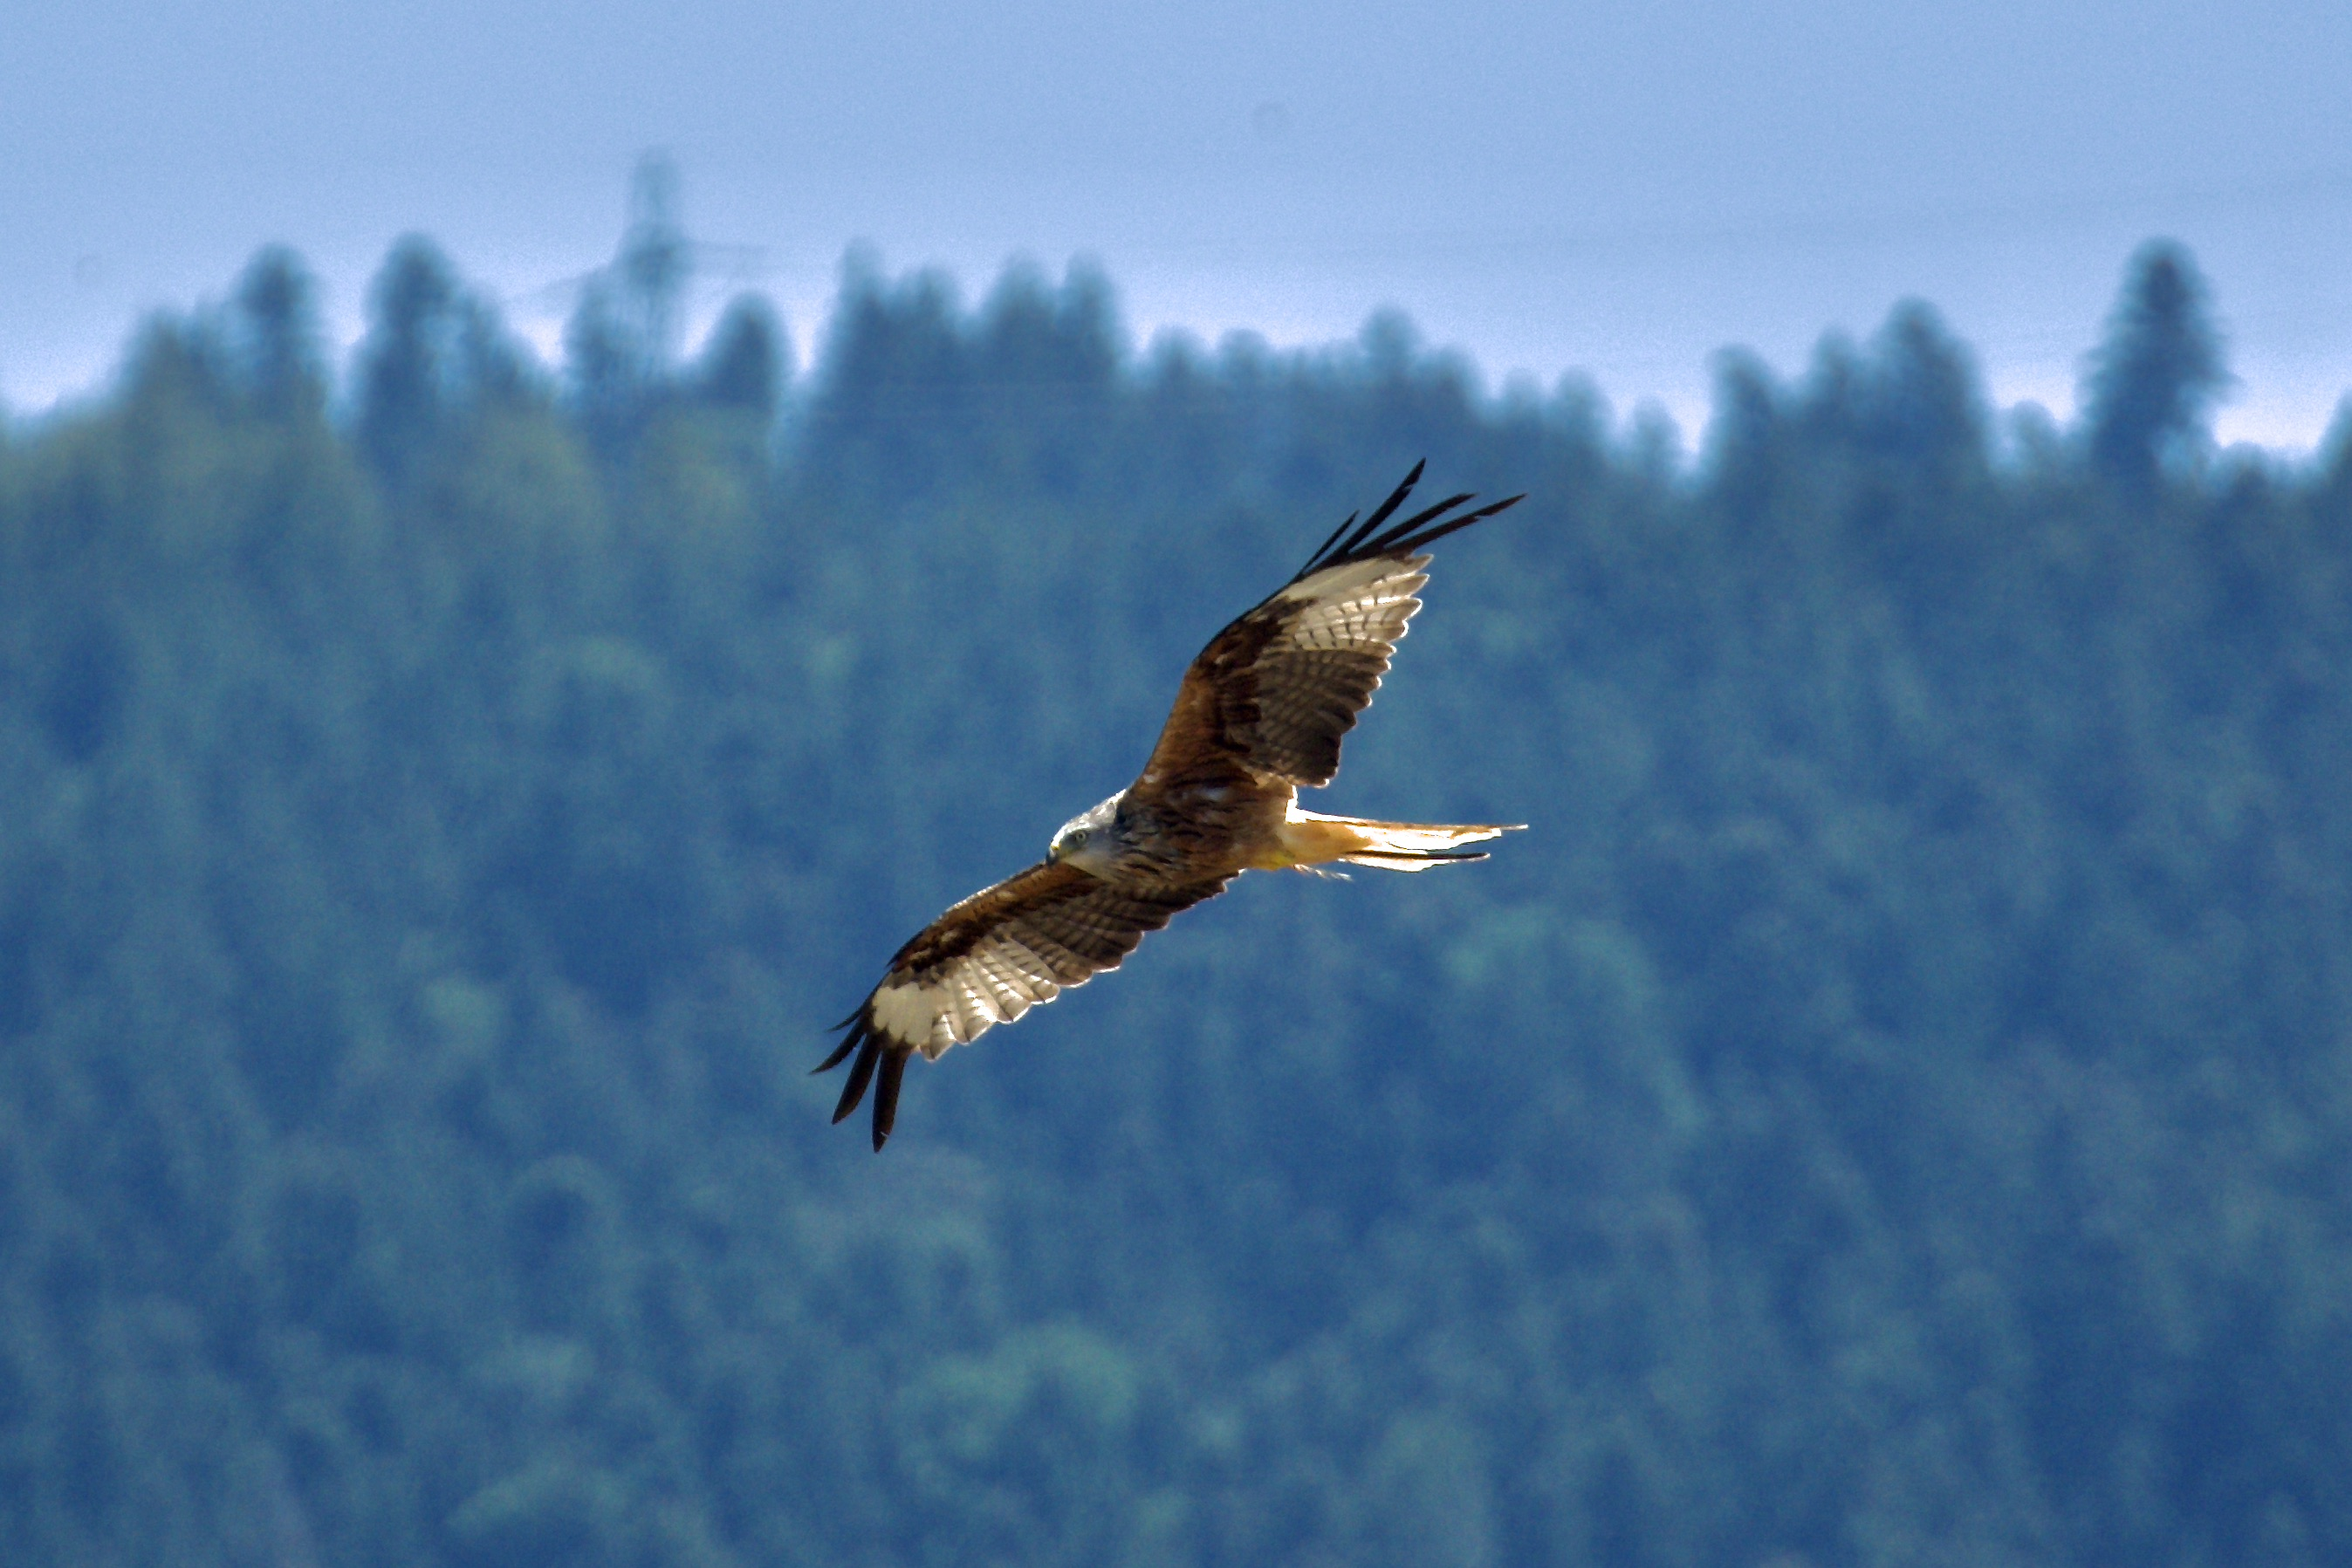
\includegraphics[width=0.495\textwidth]{figures/background/Red_kite_bottom.jpeg}
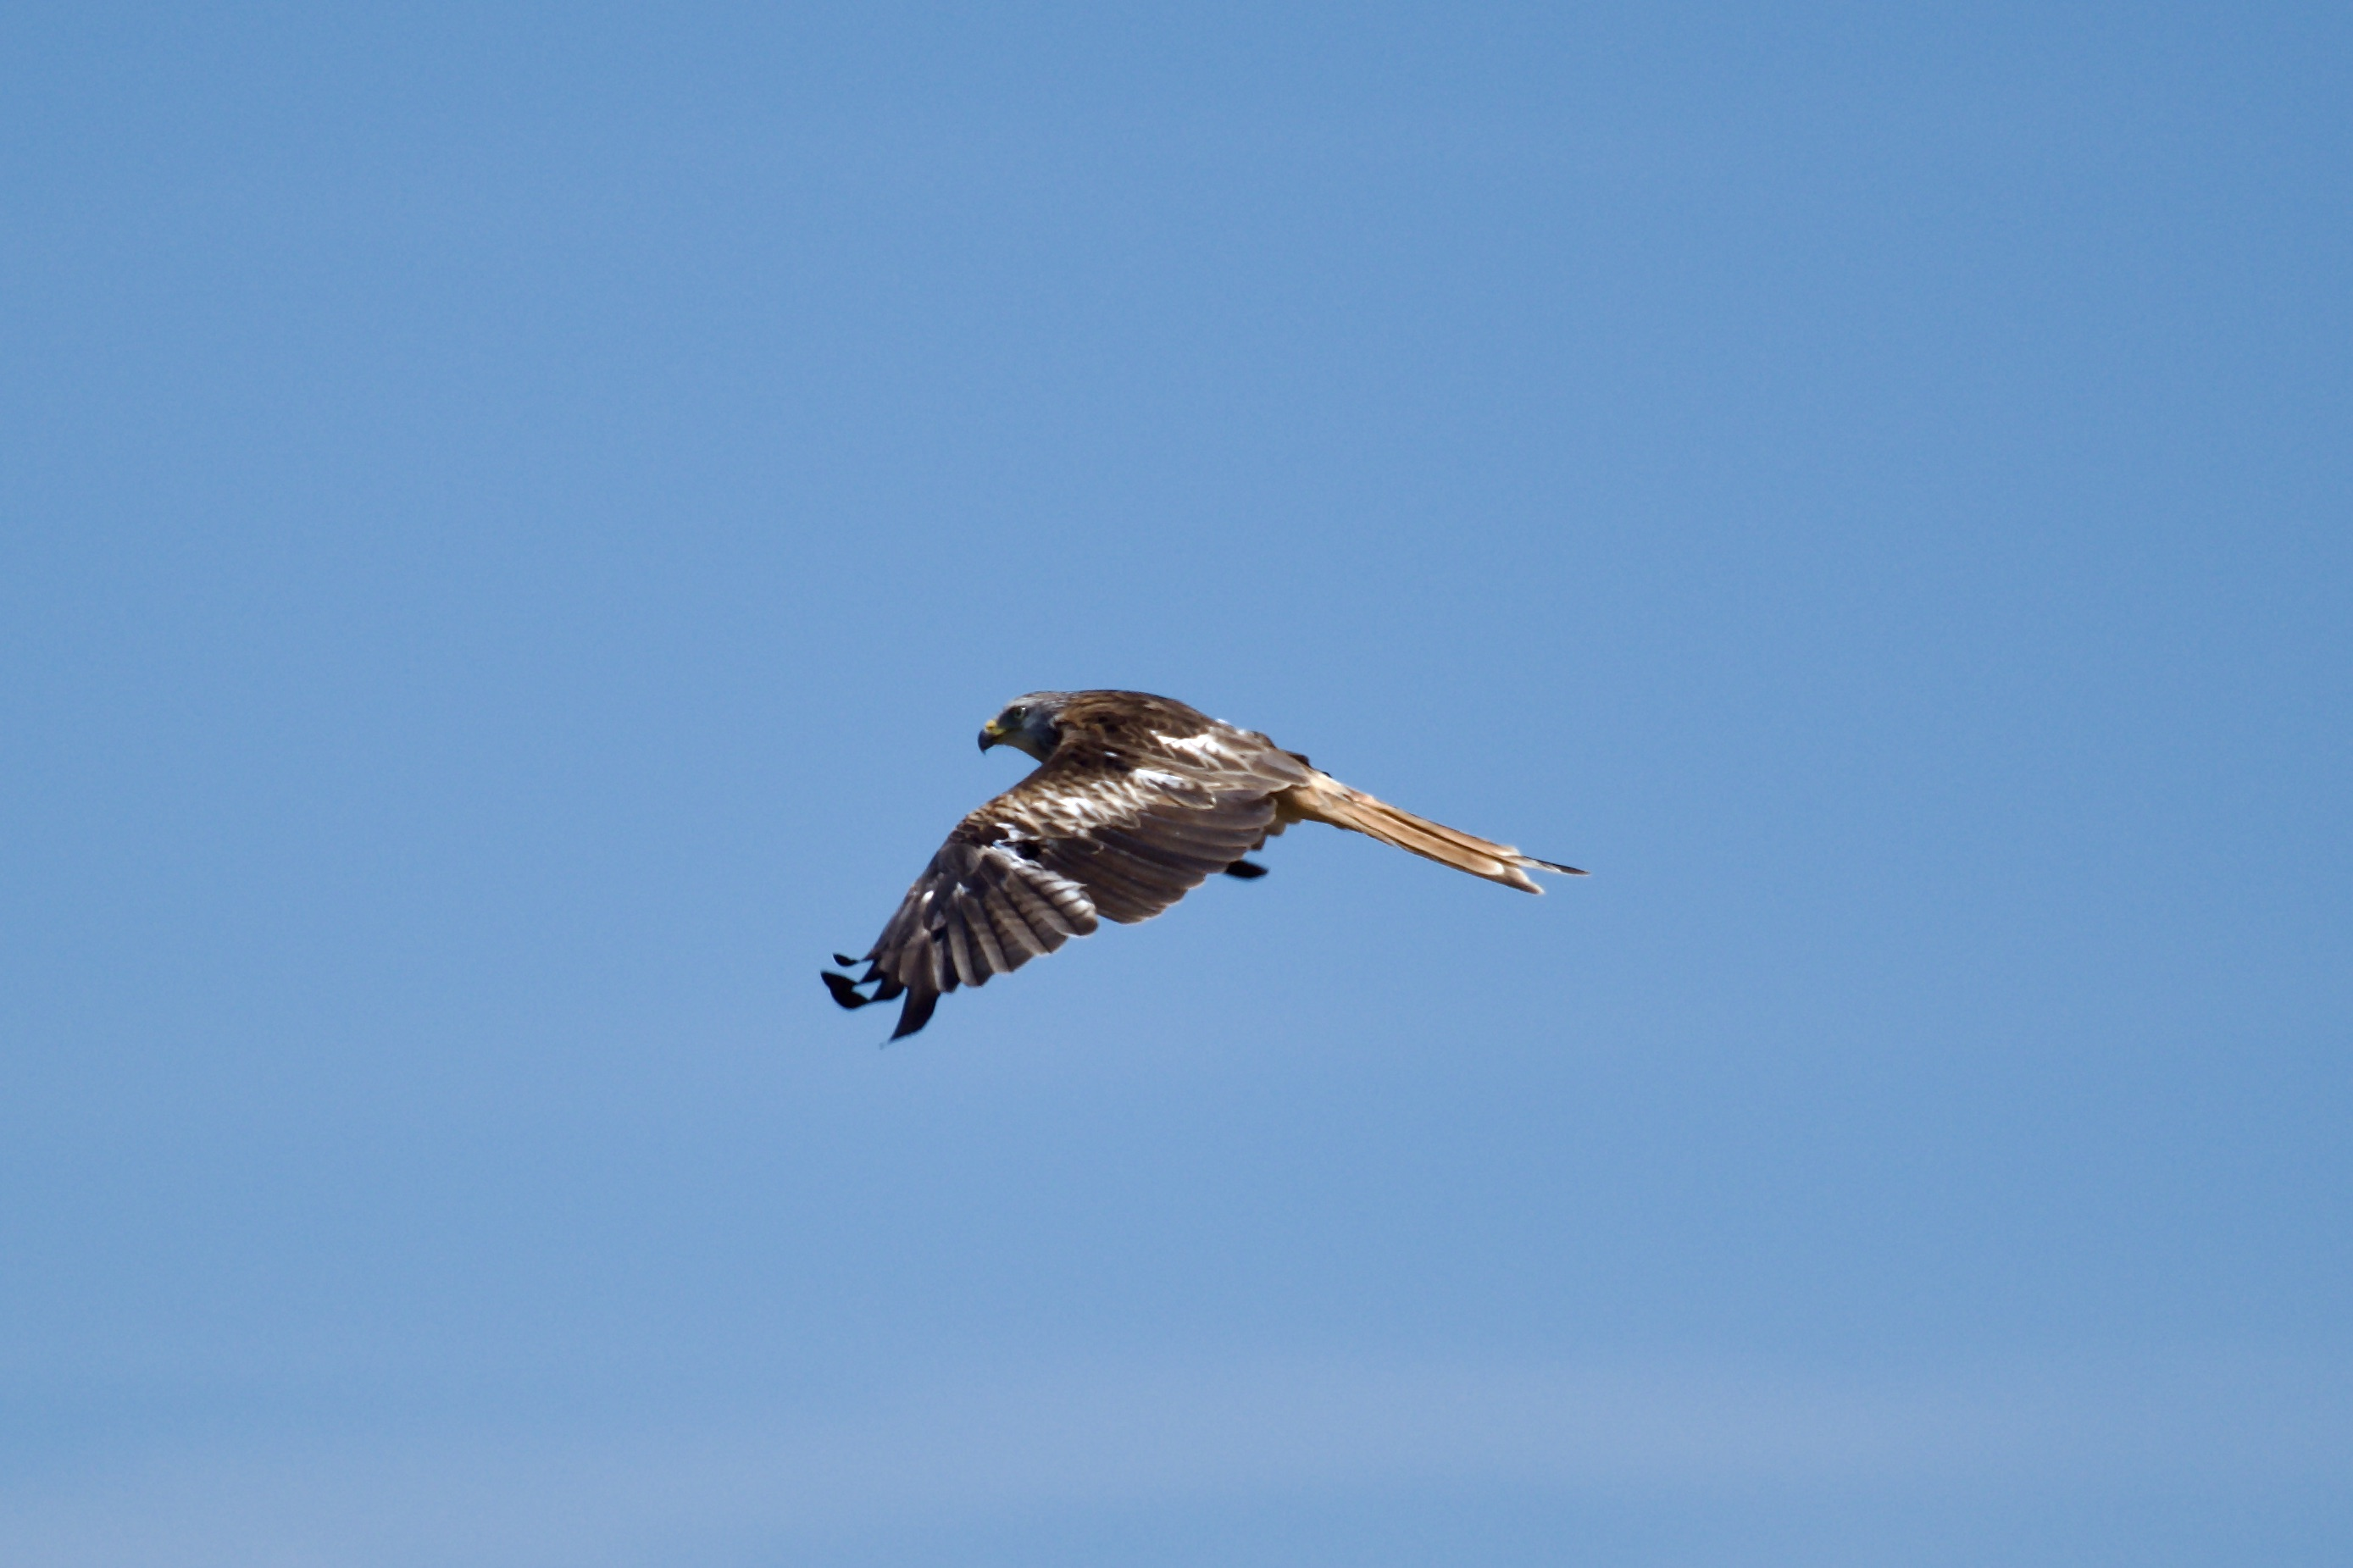
\includegraphics[width=0.495\textwidth]{figures/background/Red_kite_top.jpeg}
\caption[Red kites in flight]{Red kites in flight. Image credit: U. Beeli.}
\label{figure:red_kites}
\end{figure}

\subsubsection{Habitat}
Red kites hunt in open areas and nest in tall trees, which is why they prefer diversely structured cultural landscapes with fields and fragmented forest \parencite{mougeot2011breeding}. Red kites mainly prey on small mammals and are opportunistic scavengers, feeding on a wide range of prey, also including worms, insects, fish, birds, reptiles, amphibians, and anthropogenic food \parencite{aebischer2021rotmilan, cereghetti2019quantification, orros2015widespread, welti2019carcass}. Due to the wide prey spectrum, it is likely that red kites may be less susceptible to natural fluctuations in certain food sources \parencite{aebischer2021rotmilan, mougeot2011breeding}.

\subsubsection{Life History}
Red kites show a high variability between individuals in migration behaviour, with some individuals migrating while others remain stationary, known as partial migration \parencite{garcia2022seasonal, jaffre2013long}. Migrating birds begin the autumn migration to their wintering areas from August to November \parencite{aebischer2021rotmilan, garcia2022seasonal, pfeiffer2009satelliten}. Birds breeding in northern Europe tend to show a migratory behaviour and spend the winter months in southern Europe, mainly in southern France, on the Iberian Peninsula, in Italy and in Balkan regions as far as Greece \parencite{ferreira2015wintering, garcia2022seasonal, maciorowski2019autumn, mougeot2011breeding, panter2022age}. Birds breeding in southern Europe mostly remain in the Mediterranean region throughout the year \parencite{crespo2020analysis}, which is mainly due to the milder climate and the sufficient resource availability, making overwintering possible \parencite{garcia1998geographic}. Also in Central Europe there is an increasing number of individuals that overwinter locally and no longer migrate to southern areas \parencite{aebischer2021rotmilan}. After wintering, migrating birds begin the spring migration to their breeding areas from February to April \parencite{aebischer2021rotmilan, garcia2022seasonal, pfeiffer2009satelliten}. Red kites usually breed for the first time at the age of three to four years, but there are exceptions that start at the age of one or two years, as well as those that start later \parencite{mougeot2011breeding}. Once a breeding pair has found a home range, it is faithful to both the pair-member and the home range \parencite{aebischer2021rotmilan, mougeot2011breeding, scherler2023brutbiologie}.

\subsubsection{Reproduction} \label{reproduction}
Red kites begin to occupy their home ranges as early as February, but often not before March \parencite{aebischer2021rotmilan}. The area over which red kites forage for nesting material and food is highly dependent on habitat quality, sex and season, and can therefore vary greatly from one area to another \parencite{spatz2022sex}. Red kites do not claim a large territory exclusively, but they defend their nest fiercely against intruders from about 50-100m \parencite{aebischer2021rotmilan}. For this reason, it will be referred to a bird's activity range as its home range in this work. It is not trivial to determine the typical home range size of red kites, as there is great variability between individuals and regions. Home range sizes of 8.7--38.4 km$^2$ for males and 5.5--91.6 km$^2$ for females were obtained by \textcite{nachtigall2010aktionsraum} while home range sizes of 2.33--54.94 km$^2$ for males and 0.51--74.42 km$^2$ for females were obtained by \textcite{mammen2013rotmilan}. In a broad study, \textcite{pfeiffer2015gps} obtained home range sizes of 4.8--507.1 km2 for males and 1.1--307.3 km$^2$ for females. Besides sex and season, the size of the home range is mainly dependent on food availability, in that the area increases the scarcer the supply is \parencite{aebischer2021rotmilan, pfeiffer2015gps}. This in turn influences breeding success, which decreases significantly with increasing home range size \parencite{pfeiffer2015gps}.

A breeding pair devotes the time before breeding in their home range to preparing the nest for breeding and copulating, which can happen over 200 times per season \parencite{mougeot2000territorial}. Already before the eggs are laid, the female does not move far away from the nest and the male begins to feed her \parencite{aebischer2021rotmilan}. This behaviour, where the male gathers food while the female takes care of the nest, will also be seen later during the breeding phase \parencite{spatz2021zwischen}. Red kites build their nests mainly in tall trees, whose species can vary, in stable branch forks at a height of about 15 to 30 metres \parencite{aebischer2021rotmilan, mougeot2011breeding}. While many breeding pairs breed in the same nest every year, there are also pairs that have several nests and change them annually \parencite{aebischer2021rotmilan}.

In Switzerland, nest-building usually begins in February, while nesting material is mostly transported to the nest 30 to 40 days and sometimes even 50 days before eggs are laid \parencite{scherler2023brutbiologie}. Eggs are usually laid from the end of March and in April, while in May there are sometimes replacement broods following a first unsuccessful breeding attempt \parencite{aebischer2021rotmilan}. The clutch size is usually one to three eggs \parencite{mougeot2011breeding}. There are different values for the duration of the incubation period, ranging from 28 to 37 days, whereby it is very difficult to state an exact duration, as calculations are made partly from the laying of the first egg and partly from the laying of the last egg \parencite{aebischer2021rotmilan}. In addition, the nests are difficult to see from above and there are rarely records of monitored nests that were climbed or monitored with a camera during the laying phase \parencite{aebischer2021rotmilan}. At the beginning of the feeding phase, the female remains in the nest and food is provided by the male, while later, when the nestlings are two to three weeks old, the mother also increasingly goes foraging, but stays protectively at the nest in cold and rainy weather \parencite{aebischer2021rotmilan, spatz2021zwischen}. At about 45 days of age, the nestlings occasionally leave the nest to climb around on the branches, while at the age of seven to eight weeks they try to fly for the first time \parencite{aebischer2021rotmilan}. Basically, the breeding process of a red kite can be divided into three phases (Figure~\ref{figure:breeding_cycle}). In the first stage, a bird settles at a potential breeding site and defines its home range. In the second stage, the focus lies on the nest, which is built, improved or maintained, and finally the eggs are laid. In a third step, the breeding itself takes place, which can be divided into the two phases of hatching the eggs and feeding the nestlings. Consequently, this work will deal with the three phases individually. In the following, the term "breeding cycle" is used for all breeding-relevant steps (settlement in a home range, nest building, incubating the eggs and feeding the young birds), while the term "brood cycle" defines only the two steps of incubating the eggs and feeding the young birds.

Breeding success is complex to determine as it consists of several variables. For example, a different proportion of a bird population raises young birds in any given year. Females lay a variable number of eggs, from which a variable number of young hatch. Of these, some die during rearing, while others successfully leave the nest as fledglings. In addition, the annually varying weather conditions and food supply strongly influence breeding success \parencite{naegeli2021weather}.

After breeding, there are breeding pairs that increase their home range because they are no longer tied to the nest, while others decrease their home range because they no longer have nestlings to care for \parencite{bustamante1993post}. Some pairs stay at the nest for weeks after breeding, while others leave shortly after the young birds have become independent \parencite{paquet2015premiers, spatz2019raumnutzung}.

\vspace{1\baselineskip}

%------------------------Start of Figure------------------------
\begin{figure}[H]
\centering
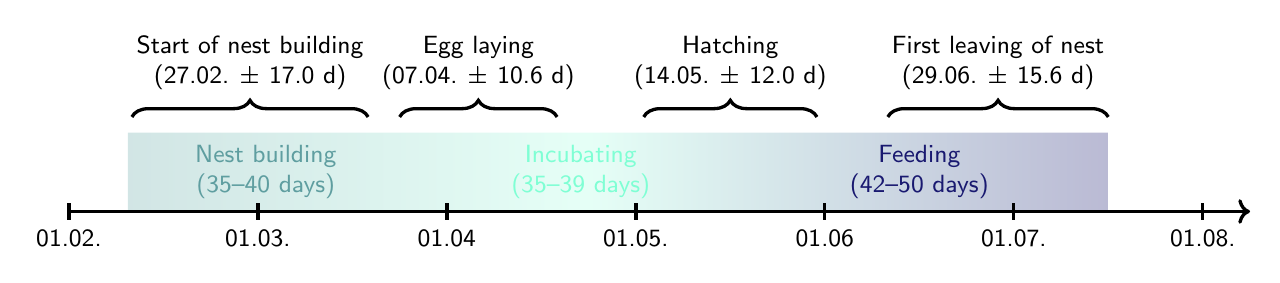
\begin{tikzpicture}[very thick, black]
\small

%% Coordinates
\coordinate (O) at (0,0); % Origin
\coordinate (P1) at (4,0);
\coordinate (P2) at (8,0);
\coordinate (P3) at (12,0);
\coordinate (F) at (15,0); %End
\coordinate (E1) at (2.3,0); %Event 1 (start nest building)
\coordinate (E2) at (5.2,0); %Event 2 (egg laying)
\coordinate (E3) at (8.4,0); %Event 3 (hatching)
\coordinate (E4) at (11.8,0); %Event 4 (leving nest)

%% Filled regions
%\shade[left color=ColorOne!30, right color=ColorTwo!20] rectangle ($(0.75,0)$) -- (P1) -- ($(P1)+(0,1)$) -- ($(0.75,0)+(0,1)$); % Nest building
%\fill[color=ColorTwo!20] rectangle (P1) -- ($(P2)+(+0.4,0)$) -- ($(P2)+(0.4,1)$) -- ($(P1)+(0,1)$); % Breeding
%\shade[left color=ColorTwo!20, right color=ColorThree!10] rectangle ($(P2)+(+0.4,0)$) -- ($(F)+(-1.8,0)$) -- ($(F)+(-1.8,1)$) -- ($(P2)+(0.4,1)$); % Feeding
\shade[left color=ColorFour!30, right color=ColorSix!30, middle color=ColorFive!20] rectangle ($(0.75,0)$) -- ($(F)+(-1.8,0)$) -- ($(F)+(-1.8,1)$) -- ($(0.75,0)+(0,1)$); % Whole breeding cycle

%% Text inside filled regions
\draw ($(P1)+(-1.5,0.5)$) node[ColorFour,align=center] {Nest building\\(35--40 days)};
\draw ($(P2)+(-1.5,0.5)$) node[ColorFive,align=center] {Incubating\\(35--39 days)};
\draw ($(P3)+(-1.2,0.5)$) node[ColorSix,align=center] {Feeding\\(42--50 days)};

%% Events
\draw [decorate,decoration={brace,amplitude=6pt}]($(E1)+(-1.5,1.2)$) -- ($(E1)+(1.5,1.2)$) node [above=6pt,align=center,black,midway] {Start of nest building\\(27.02. ± 17.0 d)};
%\draw[<-,thick,color=black] ($(E2)+(0,0.1)$) -- ($(E2)+(0,1.5)$) node [above=0pt,align=center,black] {Egg laying\\(07.04. ± 10.6 days)};
\draw [decorate,decoration={brace,amplitude=6pt}]($(E2)+(-1,1.2)$) -- ($(E2)+(1,1.2)$) node [above=6pt,align=center,black,midway] {Egg laying\\(07.04. ± 10.6 d)};
\draw [decorate,decoration={brace,amplitude=6pt}]($(E3)+(-1.1,1.2)$) -- ($(E3)+(1.1,1.2)$) node [above=6pt,align=center,black,midway] {Hatching\\(14.05. ± 12.0 d)};
\draw [decorate,decoration={brace,amplitude=6pt}]($(E4)+(-1.4,1.2)$) -- ($(E4)+(1.4,1.2)$) node [above=6pt,align=center,black,midway] {First leaving of nest\\(29.06. ± 15.6 d)};

%% Arrow (timeline)
\draw[->] (O) -- (F);
%% Ticks
\foreach \x in {0,2.4,...,14.4}
\draw(\x cm,3pt) -- (\x cm,-3pt);
%% Labels
\foreach \i \j in {0/01.02.,2.4/01.03.,4.8/01.04,7.2/01.05.,9.6/01.06,12/01.07.,14.4/01.08.}{
	\draw (\i,0) node[below=3pt] {\j} ;
}

\end{tikzpicture}

\caption[The average breeding cycle of a red kite in western Switzerland]{The average breeding cycle of a red kite in western Switzerland. In a study area of 387.5 km$^2$ in the Sense district of the canton of Fribourg and in the Gantrisch area of the canton of Bern, standardised observations of red kites were carried out by the Swiss Ornithological Institute from 2015 to 2020, which serve as a source for this figure \parencite{scherler2023brutbiologie}.}
\label{figure:breeding_cycle}

\end{figure}
%-------------------------End of Figure-------------------------

\subsection{Movement Ecology}
The research field of movement ecology studies the movement of individuals, described as a spatial change in position over time. Movement is a fundamental aspect of many life forms and is driven by both evolutionary and ecological processes, such as foraging, reproduction, or cover from predators \parencite{nathan2008movement}. In recent years, the research field of movement ecology has been revolutionised by the remote collection and analysis of large amounts of animal movement data \parencite{urbano2010wildlife,williams2020optimizing}. This evolution has been facilitated by technological advances that have led to GPS tracking devices becoming smaller and cheaper, and thus more widely applicable to smaller animals \parencite{kays2015terrestrial,tomkiewicz2010global}. Remote data collection is now used for a wide range of animal species, where initially mainly large mammals were equipped with bulky transmitters, while the ever smaller and more advanced devices are now even being used for animals in difficult environmental conditions such as marine animals and ever smaller animals such as song birds \parencite{hussey2015aquatic,kays2015terrestrial,tomkiewicz2010global}. 

This development eventually enabled the remote movement analysis of animals, which is still a relatively young field and new analysis methods are constantly evolving \parencite{nathan2013milestone}. Different aspects of an animal's life are studied that are crucial for monitoring the status and development of populations, such as migration behaviour \parencite{fudickar2021animal}, settling in a particular home range \parencite{kane2022understanding, martins2021territorial}, foraging \parencite{berger2015recursive} and reproduction \parencite{bowgen2022curves, picardi2020analysis}. Depending on the underlying motivation to move, the movement patterns often differ. Thus, different movement patterns play a role in analyses of different aspects of the life of the species under study. A specific form of movement in many animals is the revisitation of certain locations, also known as recursive movement \parencite{berger2015recursive}. Individuals often revisit specific sites, which usually represent sites of high ecological importance to them, such as foraging grounds, drinking places, or reproduction sites \parencite{bracis2018revisit}.

\subsubsection{Home Range Detection}
In the context of breeding cycle analysis, it is crucial to determine in a first step whether an individual settles in a home range where breeding may subsequently take place (Section~\ref{reproduction}). The home range of an animal can be described as the area in which the animal moves for basic daily activities, such as foraging, mating and rearing young \parencite{burt1943territoriality}. However, it can also be defined more specifically as an area where the occurrence of an animal can be indicated with a certain probability during a specific period of time \parencite{kernohan2001analysis}. This probability of an animal's occurrence in a certain place can also be understood as a density distribution. In this sense, in ecology the area in space used by an animal is called the utilisation distribution (UD) \parencite{vanwinkle1975comparison}, while it not only describes the two-dimensional movement in space, but also includes the third dimension of time, which is determined by the residence time at the visited locations \parencite{seaman1999effects}. Regardless of the exact definition, an important feature of the home range of an animal is that it is not static, but much more flexible, depending on the life status of the animal and variable between individuals of the same species \parencite{halbrook2018estimated}.

There are several different methods to determine the home range of an animal. One of the first approaches, which is still widely applied, is the Minimum Convex Polygon (MCP) \parencite{laver2008critical}. This method is very simplistic, while creating the smallest possible convex polygon around all locations, whereby no internal angle may exceed 180 degrees \parencite{burgman2003bias}. This simplicity, however, makes MCPs very sensible to spatial outliers, as the area is defined by the outermost locations \parencite{burgman2003bias}. However, this disadvantage can be counteracted by choosing a percentage level that maintains only the chosen percentages of central data points, where in ecology 95\% for a home range and 50\% for the core area of a home range are common \parencite{hasselblad2007male, houston2011breeding, kernohan2001analysis}.

Another widely used and established method, that was developed in the 1980s, is the Kernel Density Estimation (KDE), which can be used to create UDs \parencite{worton1989kernel}. KDE applies a distance weighting function where locations are weighted more heavily if they are close to clustered occurrences of several locations and weaker if they are isolated, allowing hot-spots to be identified and thus also making the method more suitable for concave geometries \parencite{laver2008critical}. This creates a smooth surface from the location point pattern, while the smoothing is controlled by a bandwidth parameter \parencite{downs2008effects}. The resulting area, which can be interpreted as the area of probability of occurrence, is usually delineated by a contour line drawn to preserve 95\% of the UD, which is usually interpreted as the home range as it eliminates outlying locations \parencite{houston2011breeding, laver2008critical}. The possibility to choose the bandwidth is the main weakness of KDEs, as the actual home range can easily be overestimated if the bandwidth is chosen too large and vice versa if the bandwidth is too small \parencite{seaman1996evaluation, worton1995using}.

Both methods also have the weakness of treating locations as independent of each other, whereas this is clearly not the case with regular GPS locations of animals \parencite{lyons2013home}. The autocorrelation of movement data depends on both the temporal and the spatial resolution \parencite{fieberg2007kernel}. As this has become an important issue, there are several approaches that address this problem, but they will not be discussed further here. Each method has its own strengths and weaknesses, which is why there is no standardised method and it should always be decided which method is most suitable depending on the application \parencite{halbrook2018estimated}.

\subsubsection{Revisitation Analysis}
Recursive movement is an essential behaviour of many animals and often takes place at sites of high ecological importance, such as foraging grounds, drinking places, or reproduction sites \parencite{barraquand2008animal, ohashi2005efficient, riotte2013periodicity}. \textcite{berger2015recursive} point out that this particular aspect of movement ecology has been underestimated by the scientific community, even though it is a basic movement behaviour shown by several different species.

\textcite{bracis2018revisit} have developed a method and integrated it into the \textit{recurse} R package that calculates revisitations based on a point-based movement trajectory. Revisitations are calculated either for each point of the trajectory or for predefined locations. Thus, either specific sites can be identified that are often visited, or the frequentation of an already known location can be analysed. With a user-specified radius, buffers are created around the locations and the entries into this area are analysed. In addition, temporal aspects of the revisitations are also calculated that provide information about the time spent at the location or the time intervals between visits. To get a meaningful result, the radius should be chosen to be larger than the measurement error of the GPS locations and not much smaller than the step length between most points, whereby the temporal resolution can also influence the choice of radius \parencite{bracis2018revisit}.

\textcite{picardi2020analysis} have developed a method to analyse the breeding success of individual birds based on a point-based movement trajectory and integrated it into the \textit{nestR} R package. An analysis of the recursions in movement trajectories of single birds is implemented in the package while a set of species-specific parameters can be adapted to the bird species studied. The output is generated through a Bayesian hierarchical model and is binary in nature while a bird either succeeded in breeding or failed. The method differs from previous research in that it also analyses the persistence of revisitations to provide information on the fate of breeding attempts \parencite{picardi2020analysis}.

\subsection{Statistical Metrics for Performance Evaluation}
The different steps of the algorithm created in this work are tested for their performance. For the categories into which the data are classified, different types of errors can be analysed. On the one hand false positives (FP), which represent cases wrongly categorised as positive, and false negatives (FN), which represent cases wrongly categorised as negative. The correctly predicted categories can be divided into true positives (TP), which represent cases correctly categorised as positive, and true negatives (TN), which represent cases correctly categorised as negative. The results can be visualised in a confusion matrix, whereas the data can be presented as counts or also as relative values \parencite{fielding_review_1997} (Table~\ref{table:conf_matrix_example}).

\begin{table}[H]
\begin{center}
\caption[Example of a 2x2 confusion matrix]{Example of a 2x2 confusion matrix.}
\label{table:conf_matrix_example}
\begin{tabularx}{0.5\textwidth} {
    | >{\centering\arraybackslash}X 
    | >{\centering\arraybackslash}X 
    | >{\centering\arraybackslash}X | }
\hline
& \textbf{Predicted \break positive} & \textbf{Predicted \break negative} \\
\hline
\textbf{Actually \break positive} &
\cellcolor[HTML]{CCFFCC} True positive (TP) & % green
\cellcolor[HTML]{FFCCCC} False negative (FN) \\  % red
\hline
\textbf{Actually \break negative} &
\cellcolor[HTML]{FFCCCC} False positive (FP) &  % red
\cellcolor[HTML]{CCFFCC} True negative (TN) \\ % green
\hline
\end{tabularx}
\end{center}
\end{table}

In order to evaluate a confusion matrix, different metrics exist. The simplest is the \textit{accuracy}, which expresses the relative number of correctly predicted cases out of all existing cases. Using this metric, it must be considered that imbalanced data can lead to misinterpretation, since accuracy treats TP and TN equally \parencite{maratea2014adjusted}. If a highly overrepresented category is correctly predicted in most cases, but an underrepresented class is mostly incorrectly predicted, the accuracy can get very high despite an actually poor performance. Accuracy is defined as follows:

\begin{equation}
Accuracy = \frac{TP + TN}{TP + FP + FN + TN}
\end{equation}

\vspace{1\baselineskip}

To evaluate the agreement of positive predictions with the observations, the metrics \textit{recall} and \textit{precision} are used. Recall provides information about the rate of correctly positive predicted cases out of all positive observations \parencite{powers2011evaluation}. Precision provides information about the rate of correctly positive predicted cases out of all positive predicted cases \parencite{powers2011evaluation}. Recall and precision are defined as follows:

\begin{equation}
Recall = \frac{TP}{TP + FN}
\end{equation}

\vspace{1\baselineskip}

\begin{equation}
Precision = \frac{TP}{TP + FP}
\end{equation}

\vspace{1\baselineskip}

The presented three metrics all range from 0 to 1, where 0 indicates complete disagreement of the predictions with the observations and 1 perfect agreement, where the values in this work are expressed as percentages. Despite their wide use in scientific literature, they are all susceptible to imbalanced data, as they do not specifically consider the agreement of the negative predicted data, in particular TN \parencite{chicco2020advantages}.

There are metrics that go further by incorporating the predictions of the negative category. One example is \textit{Cohen's Kappa}, which, in addition to the agreement of the predictions with the observations, also considers the fact that the agreement could occur by chance \parencite{cohen1960coefficient}. A similar metric is \textit{Matthews correlation coefficient (MCC)}, which, according to \textcite{chicco2021mcc}, performs even better than Cohen's Kappa. By also incorporating TN, the metrics only perform well when the majority of the predicted data is correct, in both positive and negative categories, making them highly robust for imbalanced data \parencite{chicco2020advantages, chicco2021mcc}. The result ranges from -1 (complete disagreement) over 0 (random predictions) to +1 (complete agreement) \parencite{baldi2015assessing}, where the values in this work are expressed as percentages. MCC is defined as follows:

\begin{equation}
MCC = \frac{TP \times TN-FP \times FN}{\sqrt{(TP+FP)(TP+FN)(TN+FP)(TN+FN)}}
\end{equation}

\newpage
\section{Methods}
To identify settlements in home ranges, the presence of nests and successful broods, an algorithm was developed that treats the three breeding phases separately. In the first part (Section~\ref{subsection:homerange}), individuals were identified that showed ranging behaviour consistent with settling in a home range. In the second part (Section~\ref{subsection:nest}), nest sites are located using recursive movement patterns. In the third part (Section~\ref{subsection:brood_phase_identification}), the phase of incubating the eggs and the phase of feeding the nestlings were defined based on parental movement patterns using an multinomial logistic regression model (MLRM). After the description of the data and the study areas (Section~\ref{subsection:data_study_areas}) and the pre-processing (Section~\ref{subsection:preprocessing}), the three steps of the algorithm are explained in detail. All steps carried out in this work were conducted in the R programming language for statistical computing and graphics in RStudio \parencite{rstudio}.



\subsection{Data and Study Areas}  \label{subsection:data_study_areas}
\subsubsection{Switzerland -- Main Data}
After almost becoming extinct in the 19\textsuperscript{th} and early 20\textsuperscript{th} century, increased numbers of red kite breeding pairs have repopulated the Swiss Plateau strongly, especially since the 1970s. This fact attracted particular attention, as populations in surrounding countries did not increase as much or even stagnated, of which no definite cause can be identified \parencite{swissornithologicalinstitute}. In 2015, the Swiss Ornithological Institute therefore launched a monitoring programme in the Sense region in the cantons of Bern and Fribourg to analyse population dynamics of red kites. The data collected in this project served as the basis for this work. To monitor the red kites, they were equipped with solar-powered GPS transmitters that were attached to their backs. Tagging started in 2015 and was discontinued in 2022. During this period, more than 560 individuals have been equipped with GPS transmitters, accompanied by intensive field work and data analysis. Two different models of GPS transmitters have been used in the project, Ecotone (SKUA/CREX type) since 2015 and Milsar (M9/S9 type) since 2017. While the former model collects location data at an interval of one hour, the latter has a temporal resolution of 10 minutes. In addition to the coordinates, further sensor data are collected, such as timestamp, accelerometry, or temperature. As far as the completeness was guaranteed, data from the entire project duration were used for this work in order to be able to analyse as many breeding cycles as possible. After data pre-processing, movement data of 375 breeding cycles were available, originating from 133 birds from 2016 to 2022.

As background knowledge on the individuals, valuable information was provided by the Swiss Ornithological Institute, which was collected in intensive field work. The area was divided into squares with an edge length of 2.5 kilometres, which were visited at least three times for 1-2 hours each from March to July. Using telescopes and binoculars, the red kites were observed and possibly assigned territories or even nests. Each actively used nest was visited every 1-2 weeks to observe the breeding activity, while most nests were climbed to measure and ring the fledglings and equip them with a GPS transmitter. A blood sample was taken to determine the sex of the fledglings. If the hatching date could not be observed, the age of the fledglings were derived from the weight and the wingspan measurements \parencite{scherler2023brutbiologie}. With this detailed background information, biological characteristics such as sex and age could be assigned to the GPS trajectories. Many individuals could also be assigned a home range or a nest and the timing of egg laying, chick hatching and fledging of nestlings. This information is essential for creating an algorithm to analyse the breeding process and success.

The study area of 387.5 km$^2$ extends from the Central Plateau at 482 metres above sea level to the Pre-Alps at 1763 above sea level \parencite{scherler2023brutbiologie}. The area is shaped by agriculture (56\%), managed forests (27\%), unproductive land (8.5\%) and settlements (8.5\%) \parencite{naegeli2021weather}. The diversely structured landscape with a high proportion of meadows interspersed with forests provides an ideal breeding ground for the red kite \parencite{aebischer2021rotmilan}. Most GPS locations are located in this region and most breeding takes place in this area (Figure~\ref{figure:map_breeding_area}).

\subsubsection{Germany -- Validation Data}
To test the algorithm for its performance in other geographical areas, Thomas Pfeiffer generously provided a dataset of 14 red kites during the years 2016 to 2022, of which 28 breeding cycles of 13 individuals fulfilled the requirements of the algorithm. The data stem from solar-powered GPS transmitters of red kites that bred successfully in Thuringia, Germany (Figure~\ref{figure:map_breeding_area}). Background information was also provided on the sex and timing of egg laying, chick hatching and fledging.

During the breeding season, the birds stay in Thuringia (Figure~\ref{figure:map_breeding_area}). The data points are more concentrated than in the Swiss dataset, which is due to the smaller number of birds tracked. The region in Thuringia, more specifically the Thuringian Basin, has a comparatively more homogeneous landscape structure and a relatively consistent altitude of 200 meters above sea level.

The breeding region in Thuringia, which is located east of Erfurt, lies mainly in the Thuringian Basin, which is at a relatively constant altitude of 130 to 300 metres above sea level, while in the southern part of the breeding region altitudes of over 400 metres above sea level are reached. The area contains the largest area of steppe grassland in Germany and is characterised by a warm dry climate \parencite{baumbach2013steppen}. Due to these conditions, the area is mainly used for agriculture, while there are relatively few forest areas. This landscape characteristic with large open areas leads to relatively large home ranges for red kites, which are significantly larger than for example in the breeding area in Switzerland (Figure~\ref{figure:home_range_diff_ch_de}) studied by the Swiss Ornithological Institute \parencite{aebischer2021rotmilan, pfeiffer2015gps}.

\begin{figure}[H]
\centering
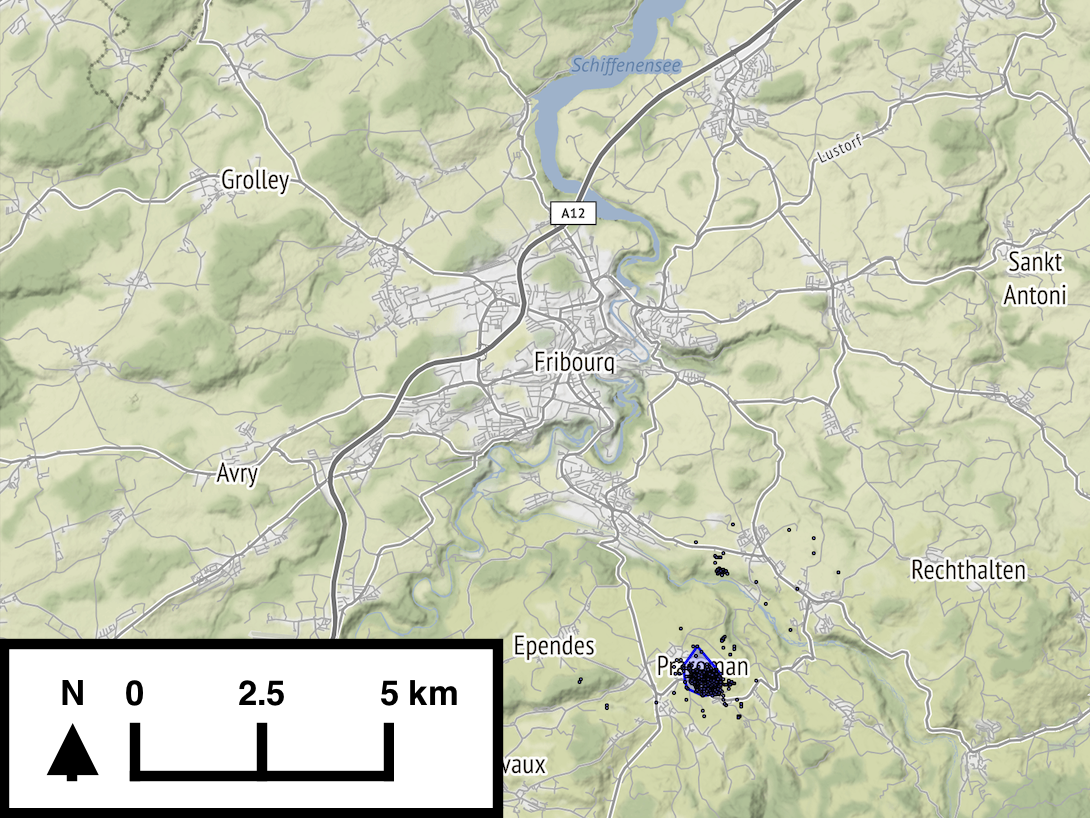
\includegraphics[width=0.495\textwidth]{figures/maps/CH_f_2022.png}
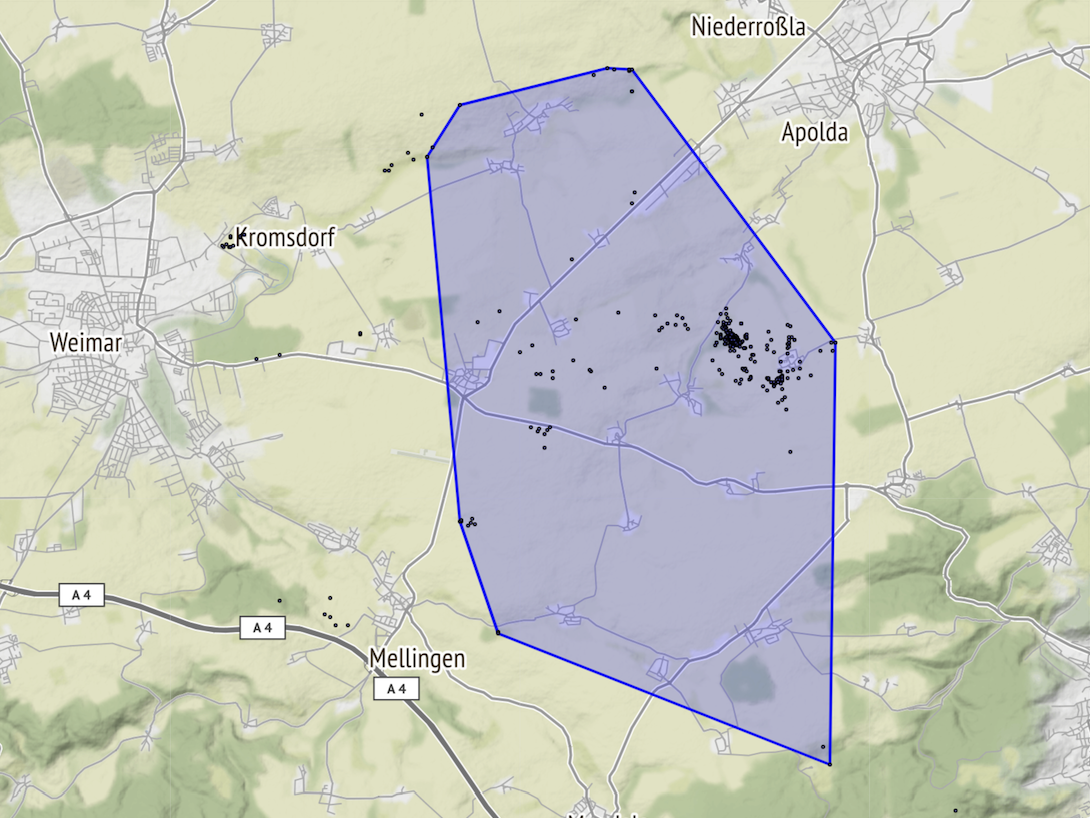
\includegraphics[width=0.495\textwidth]{figures/maps/DE_f_2022.png}
\caption[Comparison of home range sizes in Switzerland and Germany]{Home range sizes (95\% MCP) of female red kites during the breeding season 2022 in Switzerland (left) and in Germany (right). The blue areas represent the home ranges while the black points represent the GPS locations during the breeding cycle. Both maps have the same scale. Base map: Stamen.}
\label{figure:home_range_diff_ch_de}
\end{figure}

\begin{figure}[H]
\centering
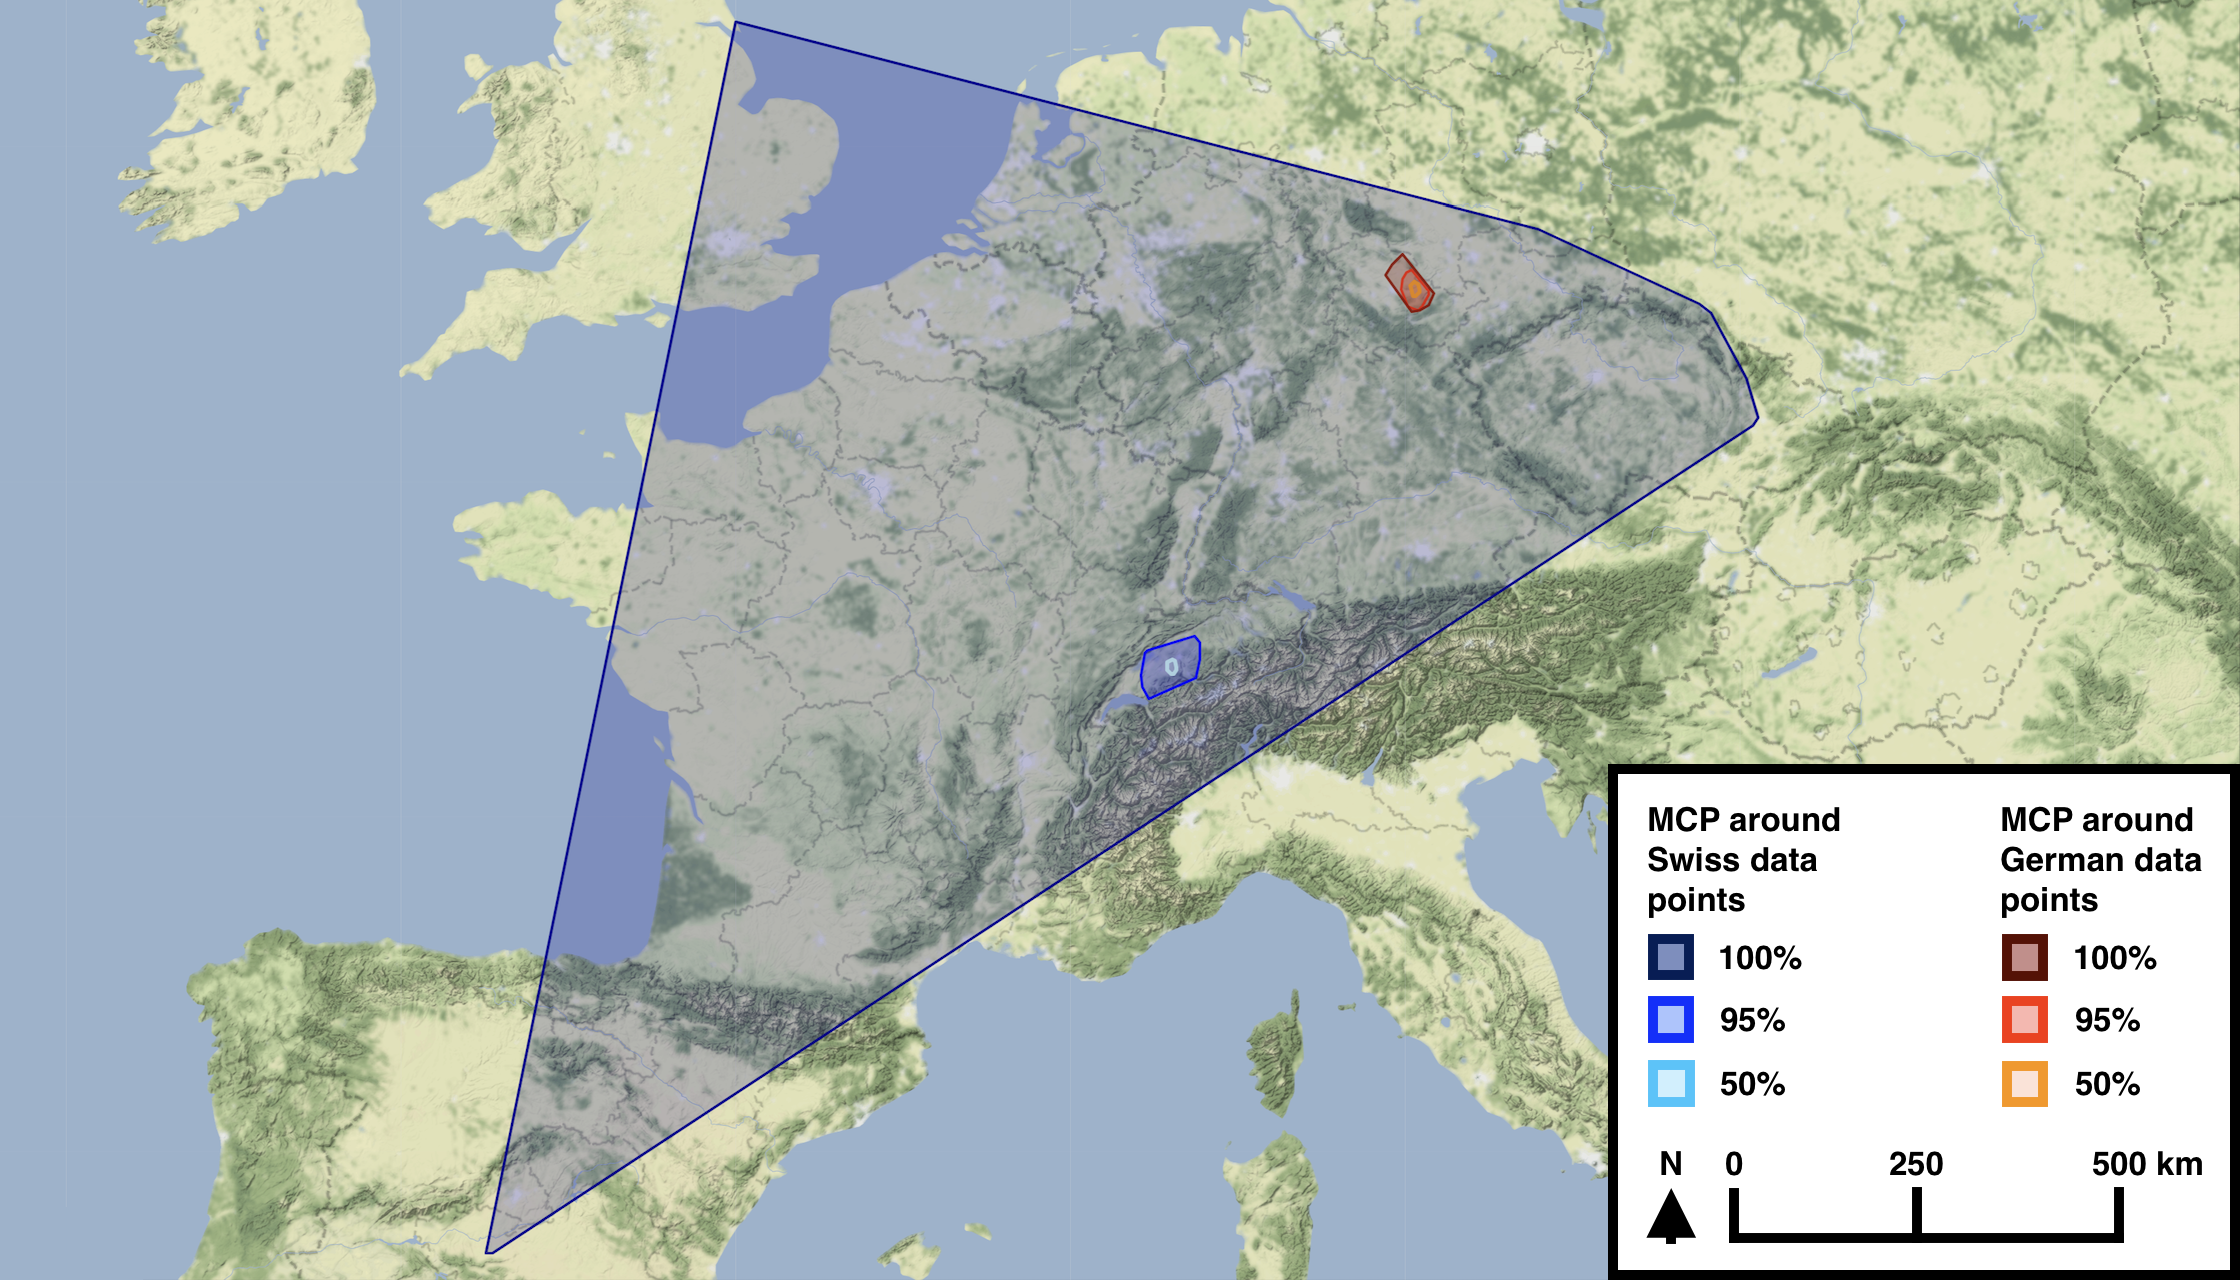
\includegraphics[width=1\textwidth]{figures/maps/All_data_MCP.png}
\caption[MCP (100\%, 95\% \& 50\%) around all red kite GPS locations of Switzerland and Germany during the breeding cycle]{MCP (100\%, 95\% \& 50\%) around all red kite GPS locations of the Swiss Ornithological Institute (blue) and all red kite locations contributed by Thomas Pfeiffer (red) during the breeding cycle. Base map: Stamen.}
\label{figure:map_breeding_area}
\end{figure}



\subsection{Pre-Processing} \label{subsection:preprocessing}
Locations without timestamps or coordinates were deleted, as well as duplicates. The dataset was reduced to the period from 1 February to 15 August to fully cover the  breeding period of red kites \parencite{aebischer2021rotmilan}. Spatial outliers were eliminated by only considering data in Europe with a buffer of 100 kilometres corresponding to the distributional range of red kites \parencite{garcia2022seasonal, literak2022disperal, mougeot2011breeding, panter2022age, seoane2003effects}. Temporal outliers were deleted, which could be defined by velocities between consecutive locations that exceed realistic flight speeds of red kites \parencite{garcia2022seasonal}. GPS locations were resampled to a temporal resolution of one-hour intervals to account for differences in sampling regime and divided into bursts. A burst is defined as a sequence of consecutive locations of the same bird that does not have a gap. Only bursts with a minimum of three locations were considered. Finally, the data was transformed from WGS84 (EPSG: 4326) to the equidistant ETRS89-extended (EPSG: 3035), to calculate realistic distance measures.



\subsection{Home Range Detection} \label{subsection:homerange}
For the detection of the home range, only data during the months of February, March, April and May were considered, as red kites occupy their home range during this period. Birds with less than 14 days of data were removed, because the algorithm requires two weeks of data to detect a potential settlement.

To determine whether a bird has occupied a territory, two parameters were used. Firstly, the area used by the individual was determined, as this can provide information about whether a bird has settled in a territory or not. Red kites reduce the spatial range of their movements upon establishing a home range containing a potential breeding site and resources \parencite{spatz2022sex}. Furthermore, the spatial displacement of the calculated area was also analysed to exclude cases where an individual may have a small home range but constantly relocates to a different area and thus, cannot have settled in a territory. To find suitable thresholds for the parameters used, the breeding data based on observations were used (Red Kite Project of the Swiss Ornithological Institute).

To calculate the home range area, 95\% MCP was used, since a rough guide value of the actual home range is sufficient for the detection of a home range in this work, and MCP is easier to parameterise than other home range detection methods. Calculating 95\% MCPs to define home ranges is a common arbitrary standard in movement ecology \parencite{fieberg2007kernel, hasselblad2007male, kernohan2001analysis, laver2008critical, signer2021fresh}. This approach saves a lot of computing power compared to more advanced metrics, yielding comparable results. To calculate the spatial displacement, the centoids of the MCPs were calculated, which then allows distance determinations between the calculated MCPs. Both parameters were calculated with the R package \textit{amt} by \textcite{signer2019amt}.

To determine the moment of settlement in time, an MCP was calculated for each bird and week. Then, with the expectation that the home range of most birds will decrease with a settlement, a threshold was identified for the MCP area below which a settlement can be assumed. Values from 10 to 100 km$^2$ were tested in steps of 10. Since a settlement cannot be assumed if only one week meets the requirement, the number of consecutive weeks that fall below the tested area values was calculated. The appropriate MCP area value combined with the optimal number of consecutive weeks was then determined by means of a visual change point detection (Figure~\ref{figure:hr_area_weeks}). The analysis showed that the threshold values of an MCP area of below 60~km$^2$ for at least 3 consecutive weeks must be met for settlement in a home range to be possible. In a final step, in order to remove birds that fulfilled the previous requirements but shifted their home range each week, a threshold value for centroid displacement was determined, which must not be exceeded for a settlement to be assumed. This distance value was also visually identified using a change point detection (Figure~\ref{figure:centroid_displacement}). The analysis showed that the minimum displacement of the calculated home ranges for all consecutive weeks in which they meet the area requirement must not exceed 760~m.

For all 908 cases for which a home range detection was carried out, the differences between the two categories (whether a home range was occupied or not according to the validation data) were analysed regarding both the number of consecutive weeks spent in an area of less than 60 km$^2$ and the centroid displacement between the respective areas. In addition, the difference between the sexes was examined.

\begin{figure}[H]
\centering
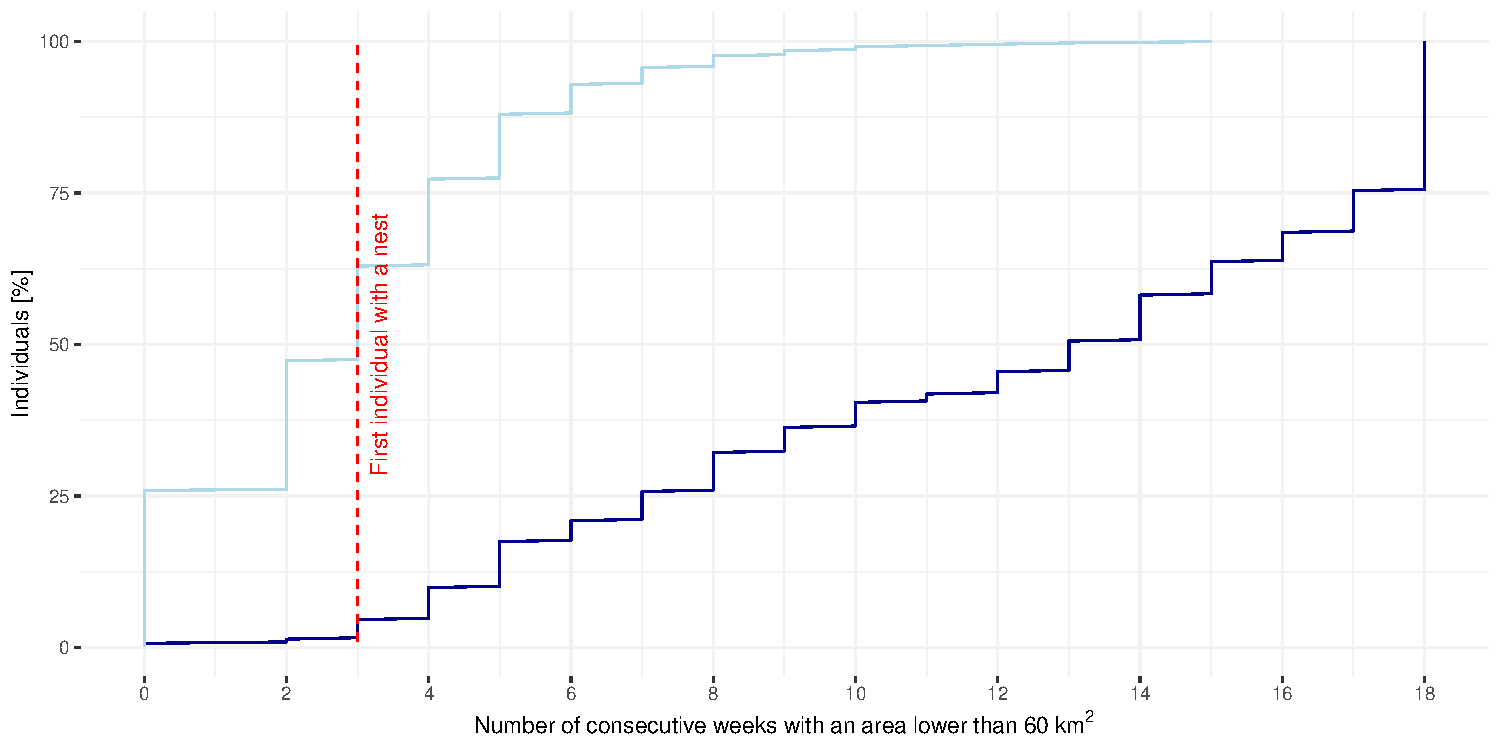
\includegraphics[width=1\textwidth]{figures/methods/01_size_60consecutive.pdf}
\caption[Change point detection for the number of weeks with an MCP < 60~km$^2$]{Visual analysis of a change point detection for the number of consecutive weeks where the MCP area is smaller than 60~km$^2$. Different colours depict the two categories of birds (dark blue = home range, light blue = no home range). The dashed red line shows the lowest number of consecutive weeks for a bird with a nest, which indicates the threshold value to filter out the highest possible number of individuals without a home range, while retaining all the individuals with a home range.}
\label{figure:hr_area_weeks}
\end{figure}

\begin{figure}[H]
\centering
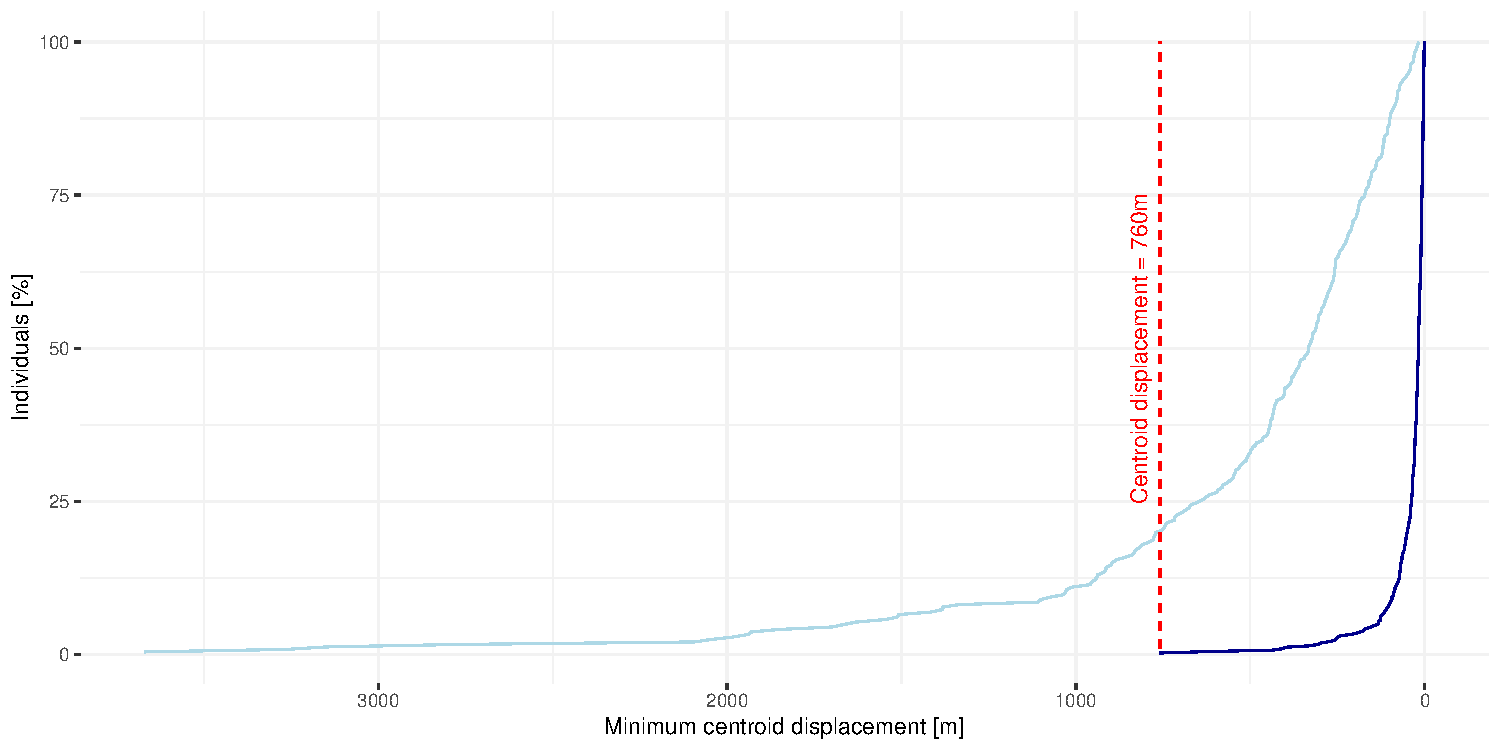
\includegraphics[width=1\textwidth]{figures/methods/03_centroid_displacement.pdf}
\caption[Change point detection for the minimum centroid displacement between weeks from a settlement onwards]{Visual analysis of a change point detection for the minimum centroid displacement between weeks from a settlement onwards. Different colours depict the two categories of birds (dark blue = home range, light blue = no home range). The dashed red line shows the threshold value that filters out the highest possible number of individuals without a home range, while retaining all the individuals with a home range.}
\label{figure:centroid_displacement}
\end{figure}



\newpage
\subsection{Nest Detection} \label{subsection:nest}
The aim of the nest detection is firstly to find out for all individuals whether they have a nest or not, and secondly to locate the potential nest. Only data during the months of March, April, May and June were considered, as this is the core phase of breeding when all breeding individuals are expected to be in the vicinity of the nest \parencite{aebischer2021rotmilan}. Although there are individuals that are at the nest much earlier, there are also those that are still in their wintering area in February. As a result, there are cases where birds repeatedly visit the same place, for example a feeding site, in their wintering area. When these birds later breed in their breeding area, the lack of sunlight under the canopy and the long time spent in the nest can lead to missing GPS data. As a result, the frequently visited site in the actual wintering area could then be wrongly identified as a nest due to the availability of more data. To avoid this particular case, the data in this step are only taken into account from March onward. In the later summer months, the same behaviour can lead to the same error, which is why these months are also not considered, as nest building in July and later are unlikely. Furthermore, for each bird individually, the data before the first week in which it settled in its home range were deleted, as territory occupation was assumed a prerequisite to nest building. For nest detection, it was also important to remove the locations recorded during the night and during twilight. The purpose of this step was to eliminate locations away from the actual nest. Especially at the beginning of the breeding phase, while the nest is still being built, some birds tend to spend the night at a roosting place which they share with other red kites \parencite{aebischer2021rotmilan}. This revisited site could easily be mistaken for the actual nest location. The night locations were calculated with the function \textit{time\_of\_day} of the R Package \textit{amt} by \textcite{signer2019amt}.

To determine whether a bird has a nest, revisitations and residence time were calculated for each GPS position using the R package \textit{recurse} by \parencite{bracis2018revisit}, as the nest is the place that is naturally visited the most during the breeding period. To find suitable thresholds for the parameters used, the validation data of the Swiss Ornithological Institute were used.

Using the function \textit{getRecursions}, the movement trajectory for each red kite and each year was analysed. With a buffer of 50~m, the number of revisitations and residence time were calculated for each point of the trajectory. The buffer size of 50~m was chosen because the radius should not be much smaller than most distances between locations and should also be larger than the measurement error \parencite{bracis2018revisit}.

Highly frequented sites do not necessarily represent an actual nest. Non-breeding individuals that have not occupied a home range may move over large areas but still frequent certain locations. Breeding individuals, on the other hand, stay mainly in the vicinity of the nest, which is why an accumulation of highly frequented sites around the nest location is expected to be seen in the data. In order to localise the area around the nest and to exclude possible frequently visited sites before and after breeding, the area covered by the most visited sites was calculated for each individual. The optimal number of most visited locations and the size of the area they cover were the subject of a further visual change point detection (Figure~\ref{figure:nest_area_45}). The analysis showed that the threshold values of 45 most visited locations, covering an area of less than 0.052~km$^2$, were the most suitable for distinguishing individuals with a nest from individuals without one.

From the remaining individuals, the potential nest site was then determined. The most visited location was assumed to be the nest site. If several locations had the same value, the one with the longest residence time was chosen.

In order to find out whether the most visited location was sufficiently visited and enough time was spent there to represent a nest, a second revisitation analysis was carried out. This time, the revisitation analysis focused on the predicted nest location with a buffer radius of 50 metres. The function \textit{getRecursionsAtLocations} was used for this purpose. For each day it was calculated how often the predicted nest location was visited and how much time was spent there. From this, a relative value for the average daily revisitations and the average daily residence time was calculated over the entire period in which data were available. Suitable threshold values that must be reached were again selected by means of a visual change point detection (Figure~\ref{figure:revisits_cpd}~and~\ref{figure:residence_time_cpd}). The analysis showed that the most frequently revisited locations must be revisited at least 0.54 times per day and for at least 31 minutes per day to represent a potential nest.

For all 624 cases for which a nest detection was carried out, the differences between the two categories (whether a nest was present or not according to the validation data) were analysed regarding residence time and revisitations. In addition, the difference between the sexes was examined.

\begin{figure}[H]
\centering
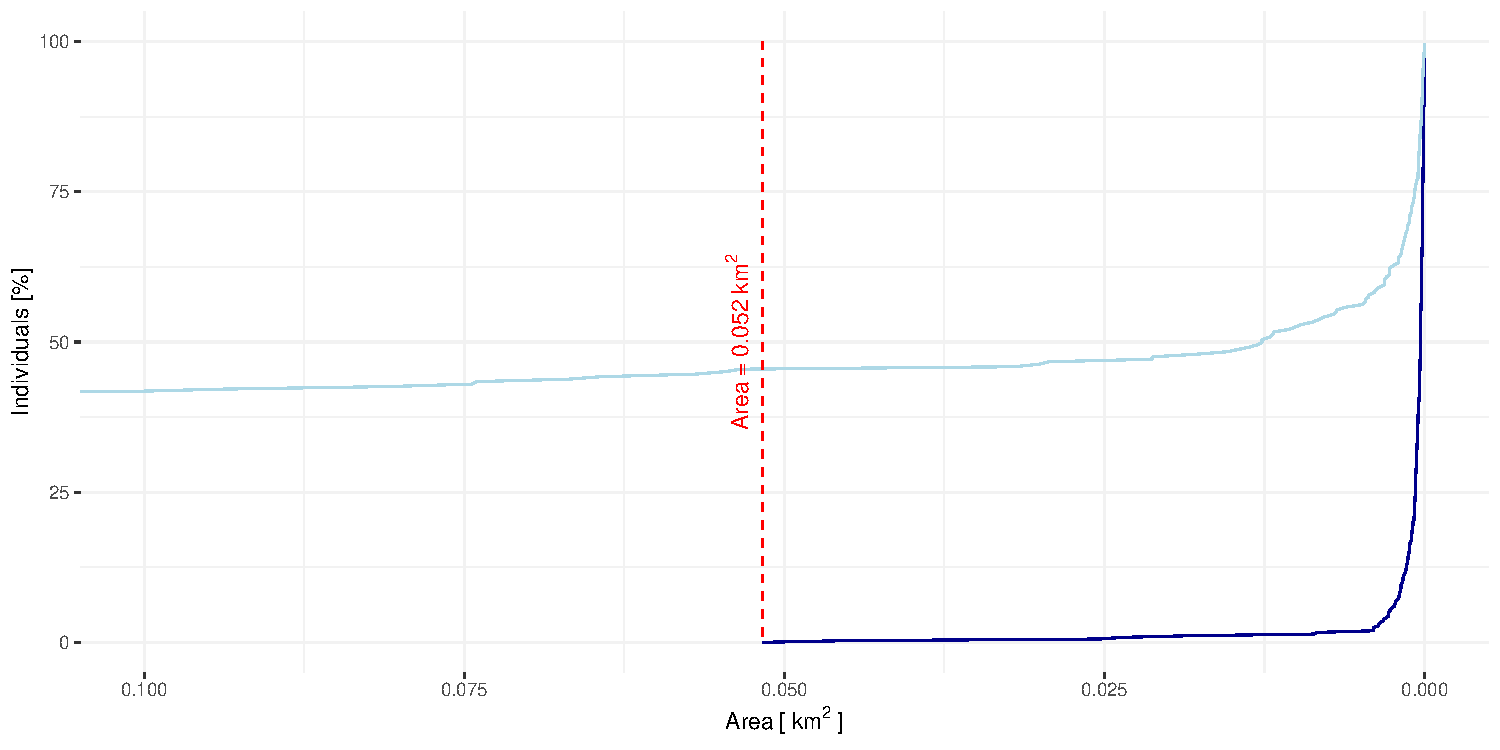
\includegraphics[width=1\textwidth]{figures/methods/01_area_45_most_visited.pdf}
\caption[Change point detection for the size of the area of the 45 most visited locations]{Visual analysis of a change point detection for the size of the area of the 45 most visited locations. Different colours depict the two categories of birds (dark blue = home range, light blue = no home range). The dashed red line shows the highest area value for a bird with a nest, which indicates the threshold value to filter out the highest possible number of individuals without a nest, while retaining all the individuals with a nest.}
\label{figure:nest_area_45}
\end{figure}

\begin{figure}[H]
\centering
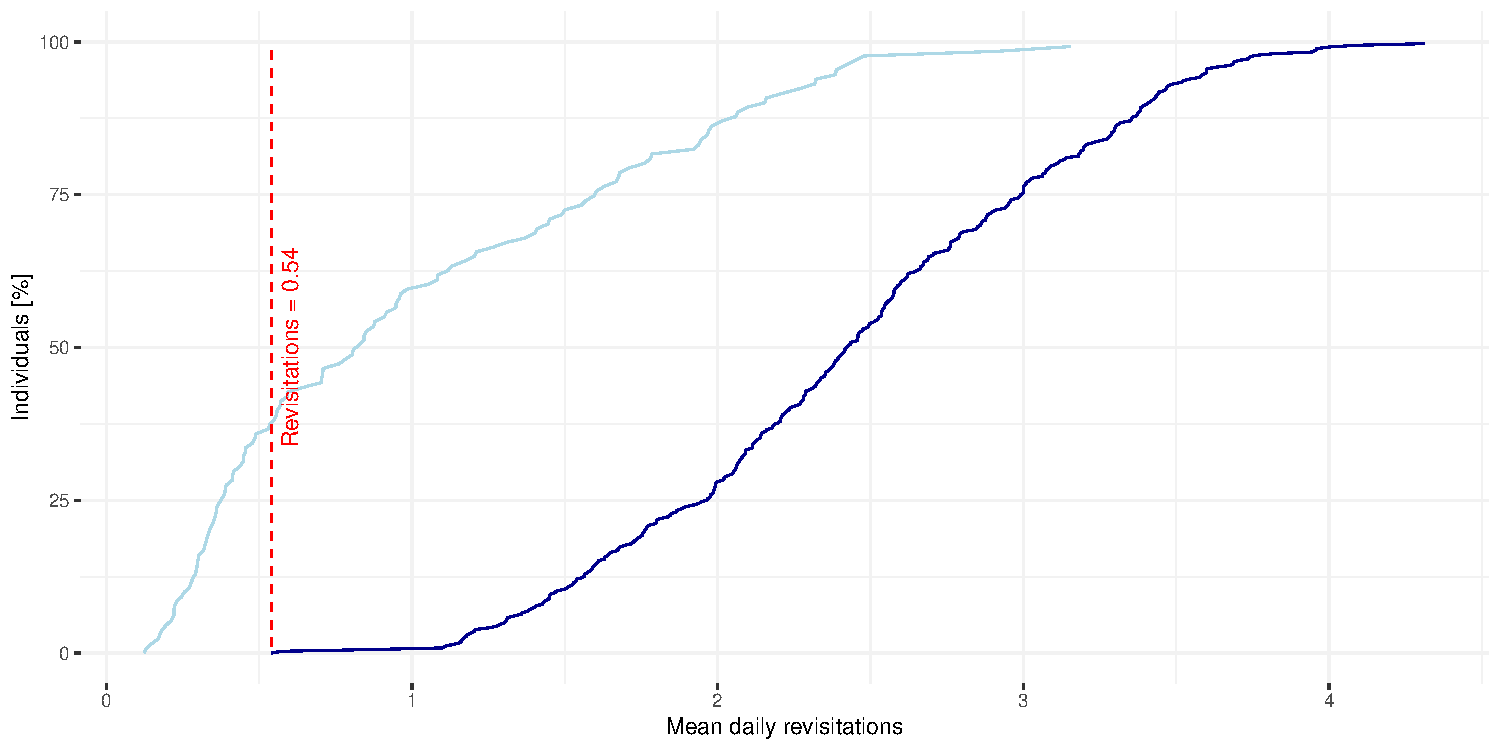
\includegraphics[width=1\textwidth]{figures/methods/06_revisits.pdf}
\caption[Change point detection for the mean daily revisitations at the predicted nest location]{Visual analysis of a change point detection for the mean daily revisitations at the predicted nest location. Different colours depict the two categories of birds (dark blue = home range, light blue = no home range). The dashed red line shows the lowest number of mean daily revisitations for a bird with a nest, which indicates the threshold value to filter out the highest possible number of individuals without a nest, while retaining all the individuals with a nest.}
\label{figure:revisits_cpd}
\end{figure}

\begin{figure}[H]
\centering
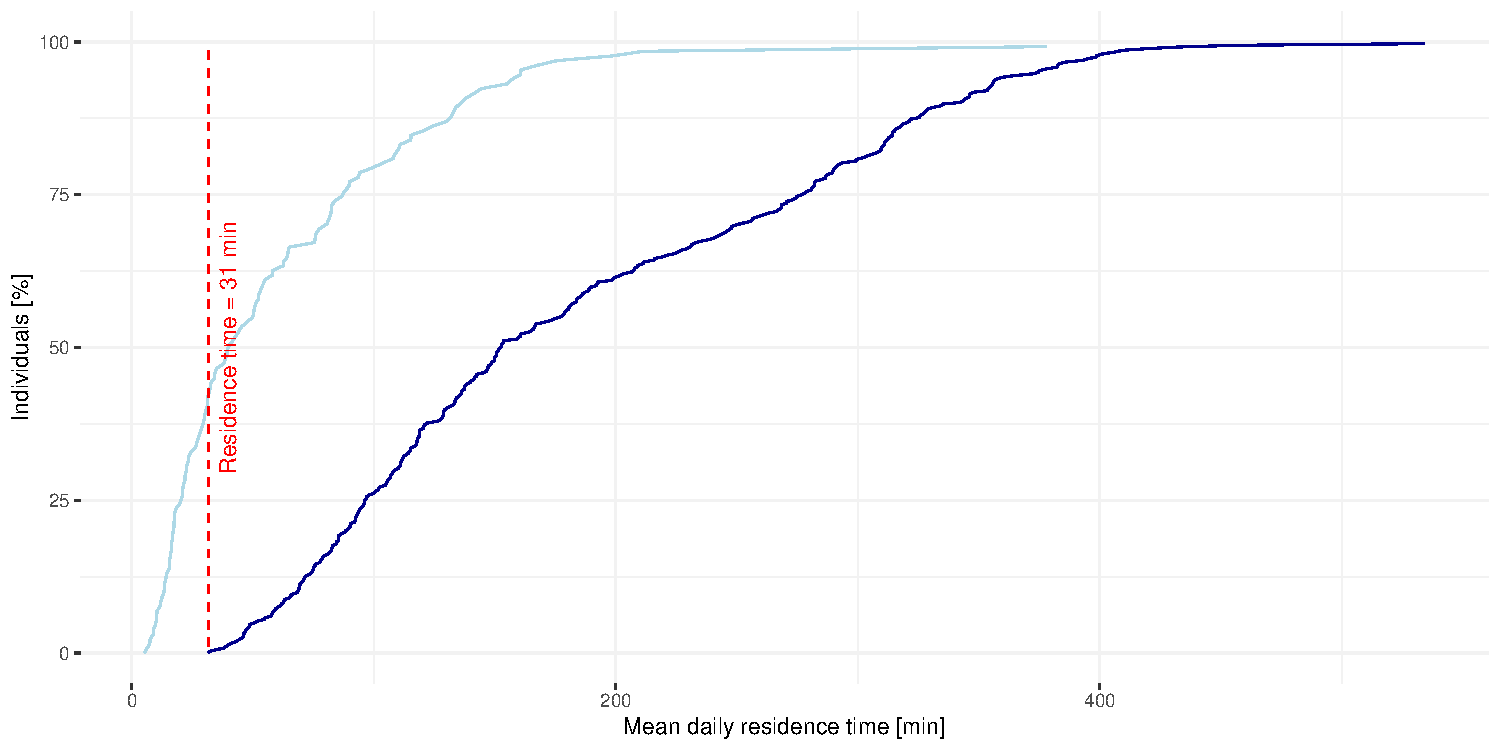
\includegraphics[width=1\textwidth]{figures/methods/04_residence_time.pdf}
\caption[Change point detection for the mean daily residence time at the predicted nest location]{Visual analysis of a change point detection for the mean daily residence time at the predicted nest location. Different colours depict the two categories of birds (dark blue = home range, light blue = no home range). The dashed red line shows the lowest mean daily residence time for a bird with a nest, which indicates the threshold value to filter out the highest possible number of individuals without a nest, while retaining all the individuals with a nest.}
\label{figure:residence_time_cpd}
\end{figure}



\subsection{Brood Phase Identification} \label{subsection:brood_phase_identification}
The aim of the brood phase identification is to identify the two phases of incubating the eggs and feeding the nestlings during a brood cycle. The duration of these two phases is then used to distinguish successful broods from unsuccessful broods.

To detect the two phases of incubating and feeding, the aim was to predict separately for each day of a brood cycle whether an individual was incubating, feeding or not breeding (this last category will from here on be referred to as non-breeding). To classify a day into one of the three categories, the probability of classification into each of the categories should be calculated for the movement pattern on that day. The percentages of the different categories on a day would then make it possible to classify the day into one of the categories. Calculating probabilities instead of assigning the day directly to a category offers the advantage that with breeding biology background knowledge, the categories can be meaningfully classified through an interpretation of the predictions or a rule-based approach.

There are numerous classification methods that allow daily movement patterns to be assigned to one of the three categories mentioned. For the sake of simplicity, only the chosen method is explained here, highlighting its specific advantages. The approach of using a multinomial logistic regression model (MLRM) was chosen, which is characterised by the fact that, compared to a binomial logistic regression model, the response variable is defined in more than two non-ordinal categories \parencite{kwak2002multinomial}. This approach can be particularly advantageous as it means that there is no need to collapse several categories in order to use the widely used and more familiar binomial logistic regression model \parencite{kwak2002multinomial}. The MLRM was generated with the R package \textit{brms} by \textcite{buerkner2017brms}. The package \textit{brms}, allows to use Bayesian multilevel models in R based on the probabilistic programming language \textit{Stan}. The advantage of the Bayesian implementation is the fact that it is based on probability distributions, which is particularly suitable for this work, as it allows probabilistic predictions and a final interpretation of the predictions.



\subsubsection{Data Pre-Processing for the MLRM} \label{subsubsection:mlrm_preprocessing}
To train the MLRM, only data from 10 March until 31 July were considered, as this is the period in which the entire brood cycle of the vast majority of red kites takes place. In western Switzerland, no start of breeding has yet been observed before 14 March \parencite{scherler2023brutbiologie}. The date was rounded off to 10 March to create a buffer for unexpected special cases. By the end of July, basically all the young birds have fledged \parencite{aebischer2021rotmilan}. To ensure that the model was created with a sufficiently detailed dataset, the data were subjected to further requirements. Firstly, the individuals considered had to provide at least one day of data in each of the months considered. Secondly, days with less than three GPS locations were filtered out, as this is the minimum requirement for calculating an area. Finally, the number of days (143) was multiplied by three locations, which was then used as the minimum number of GPS locations that must be present over the entire period (429). In addition, sufficient validation data had to be available on the duration of incubation and feeding or the date of egg laying, the hatching date and the date when the young birds left the nest. This resulted in a dataset of 222 brood cycles from 102 individuals with sufficient data and information. Exactly half of the breeding cycles stem from females and the other half from males.

The response variable of the MLRM is the brood phase, which is predicted on a daily basis and has three categories: breeding, feeding and non-breeding. Several explanatory variables were calculated that could be suitable for integration into the MLRM from a biological perspective. All variables were calculated on a daily basis to meet the model's requirement to calculate predictions on a daily basis. The explanatory variables calculated were 95\% MCP, revisitation at the nest location, residence time at the nest location, distance to the nest location, and step length between GPS locations. MCPs and step lengths were calculated with the R package \textit{amt} by \textcite{signer2019amt}, revisitations and residence time with the R package \textit{recurse} by \textcite{bracis2018revisit} and distance to the nest location with the R package \textit{sf} by \textcite{pebesma2018simple}. In addition, the two movement-independent variables sex and sensor temperature were included. Sex was included due to the different roles of the parents during the brood cycle \parencite{spatz2021zwischen}, while the body temperature of females was expected to increase during breeding \parencite{aebischer2021rotmilan}. Finally, the number of GPS locations per day was defined as a control variable and an ID combining the individual and the respective year as a random effect. The number of GPS locations per day was included in the model as it was assumed to influence the accuracy of the calculation of movement patterns. The ID combining the individual and the respective year was integrated to correct for dependencies of the data, as an individual can provide data over several years.

For most variables, several variations were calculated in order to analyse which were most suitable for the final model. For step length, distance to the nest location and temperature, the daily mean, minimum and maximum values were calculated. For 95\% MCP, revisitations, residence time, distance to the nest, step length and temperature, moving average values were calculated over the previous three, five and seven days (including the day under consideration). This eliminates outliers that can be caused by individual days in which the movement behaviour deviates from the expected behaviour or the data is insufficient. For example, movement behaviour can be strongly influenced by extreme weather conditions, so that the red kites only perch at the nest during a day in order to protect their nestlings and not endanger themselves, while they would actually search for food in normal weather conditions \parencite{aebischer2021rotmilan}.

As a final step, all variables were scaled and centered. Besides the fact that this prevents convergence problems in linear models, it also makes the model applicable to other red kite populations with different dimensions of movement.



\subsubsection{Implementation of the MLRM} \label{subsubsection:mlrm_implementation}
The dataset with 222 brood cycles was divided into a training dataset (70\%, 155 brood cycles, 76 females and 79 males) and a test dataset (30\%, 67 brood cycles, 35 females and 32 males). With the developed variations of the variables (Section~\ref{subsubsection:mlrm_preprocessing}), different MLRMs were developed and trained with the training dataset.

In order to determine the most appropriate variation of each variable as explanatory variable, identical models were developed using a different variation of each variable. To determine the most appropriate variation, estimates of the variables were plotted. For each variable, it was visually determined which variation had the strongest influence on the model. The respective variation was then selected to further generate the best performing model. The variables that did not show large estimates in all variants were excluded from the further models. The variations of the explanatory variables that were ultimately used for the model are listed in Table~\ref{table:mlrm_variables}.

With the appropriate explanatory variables, several variants of models were developed in which different interactions between the variables were built in and the variables were weighted differently. This resulted in 17 different models, which were then compared with each other in terms of their performance. To compare the models with each other, the efficient approximate leave-one-out (LOO) method was used. LOO is used for cross-validation of Bayesian models. The method is implemented in the R Package \textit{brms} and is based on the description of \textcite{vehtari2017practical}, who present an efficient computation of LOO using on Pareto-smoothed importance sampling.

The best performing model included sensor temperature as an explanatory variable. However, a simpler model without sensor temperature performed similarly (the later predictions with the test dataset showed also similar results). Finally, the model without sensor temperature was selected as the appropriate model for two reasons. On the one hand, the sensor temperature is a mixed temperature of the air temperature and the body temperature. The two proportions differ according to sensors, activity of the bird, weather and season, which complicates the interpretation of the temperature. On the other hand, there are GPS transmitters without temperature sensors, for which the model can also be used. Thus, the MLRM is applicable to a wider range of data, especially older data. Due to a similar performance, the model with the fewest possible variables and consistent performance was chosen. A summary of the MLRM is shown in Appendix~\ref{appendix:mlrm_formula}. To analyse the performance of the model in terms of predictions, it was applied to the test dataset. The visual representations of the predictions of all 67 brood cycles are listed in Appendix~\ref{appendix:mlrm_predictions_test}.

\begin{table}[H]
\begin{center}
\caption[Explanatory variables of the MLRM]{Explanatory variables that were integrated in the MLRM.}
\label{table:mlrm_variables}
\begin{tabular}{| p{6cm} | p{2.5cm} | p{2.5cm} |}
\cline{1-3}
\textbf{Variable description} & \textbf{Variable type} & \textbf{Variable \newline range/levels} \\
\hline
95\% MCP \newline (moving average over 7 days) & Numeric & 0.0000003 - 1\\ 
\hline
Revisitations at nest location \newline (moving average over 7 days) & Numeric & 0 - 1 \\
\hline
Residence time at nest location \newline (moving average over 7 days) & Numeric & 0 - 1\\
\hline
Daily mean distance to nest location \newline (moving average over 7 days) & Numeric & 0.00008 -1\\
\hline
Sex & Binary & 0, 1\\
\hline
\end{tabular}
\end{center}
\end{table}



\subsubsection{Brood Success Evaluation}
In order to derive the breeding success from the raw model predictions, three approaches were used. In all three approaches, the model predictions are compared with the shortest known brood duration for this species. According to \textcite{aebischer2021rotmilan}, red kites must be incubating at least 28 days and feeding the nestlings at least 42 days in order to successfully produce fledged offspring. If an individual reached the minimum number of days in the year under consideration, it was classified as a successful brood in all three approaches.

\vspace{1\baselineskip}
\noindent \textbf{Raw Model Predictions} \newline
\noindent In this approach, the category of a day is derived directly from the raw model prediction. Every day is classified in the category that shows the highest probability value on the respective day.
The days of the respective category are then added up. When the minimum number of days per category was reached, the brood was considered successful. A visual representation of the raw model predictions compared to the validation data from the field observations can be seen in Figure~\ref{figure:example_prediction} (left).

\vspace{1\baselineskip}
\noindent \textbf{Merged Categories} \newline
\noindent In this approach, the two categories incubating and feeding are merged into a new category "breeding". Thus, there are only the two possibilities that an individual is breeding or non-breeding. This method is based on the idea that movement behaviour patterns during incubation and during feeding are similar (especially in male red kites), making these two categories easy to misclassify, but still clearly distinguishable from non-breeding. A day is categorised as non-breeding as soon as the probability is above 50\% and as breeding if the probabilities of the two categories incubating and feeding add up to at least 50\%. When the number of breeding days reach the minimum number of days of incubating and feeding combined (70 days), the brood was considered successful.

\vspace{1\baselineskip}
\noindent \textbf{Rule-Based Adaptation} \newline
\noindent In this approach, the raw model predictions were adjusted using rules based on biological knowledge on the respective breeding phase. The application of the rules is to ensure that the predictions are smoothed and outliers in the calculated movement behaviour that do not fit the expected pattern are corrected. While the predictions were manipulated, it was intended not to bias the predictions too much to match expected patterns and thus potentially distort the result. The following rules were used for this approach:

\begin{itemize}
    \item The first day of incubation must not be isolated. There have to be at least five days of incubation in a row. All previous days are reclassified to non-breeding.
    \item The last day of incubation must be no later than 39 days after the first day of incubation. All later days of incubation are reclassified to feeding.
    \item Between the first day of incubation and the last day of incubation, isolated days of feeding are reclassified to incubating.
    \item The first day after the last day of incubation is reclassified to feeding.
    \item The last day of feeding must be no later than 50 days after the first day of feeding. All later days of feeding are reclassified to non-breeding.
    \item Between the first day of incubation and the last day of feeding, single isolated non-breeding days are reclassified to the category they are located in.
\end{itemize}

\noindent A visual example of the influence of this rule-based adaptation approach on the model predictions can be seen in Figure~\ref{figure:example_prediction} (right).

\begin{figure}[H]
\centering
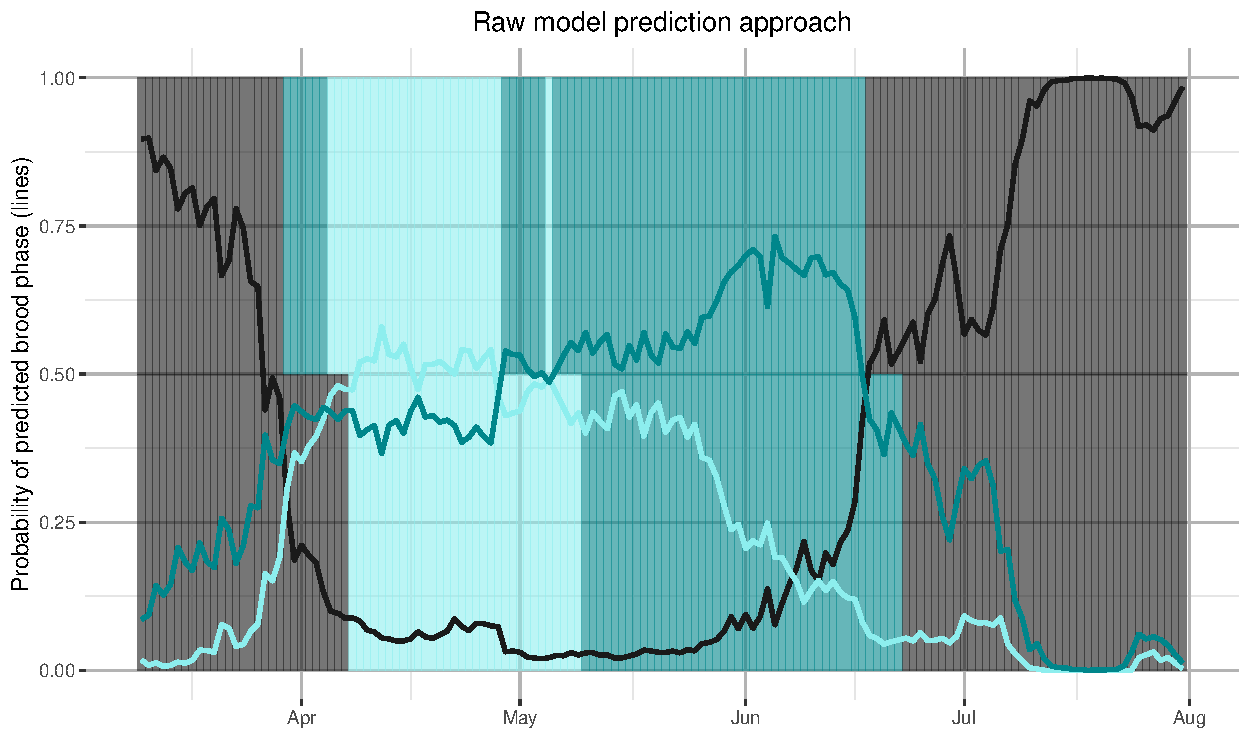
\includegraphics[width=0.45\textwidth]{figures/methods/07_prediction_example_raw.pdf}
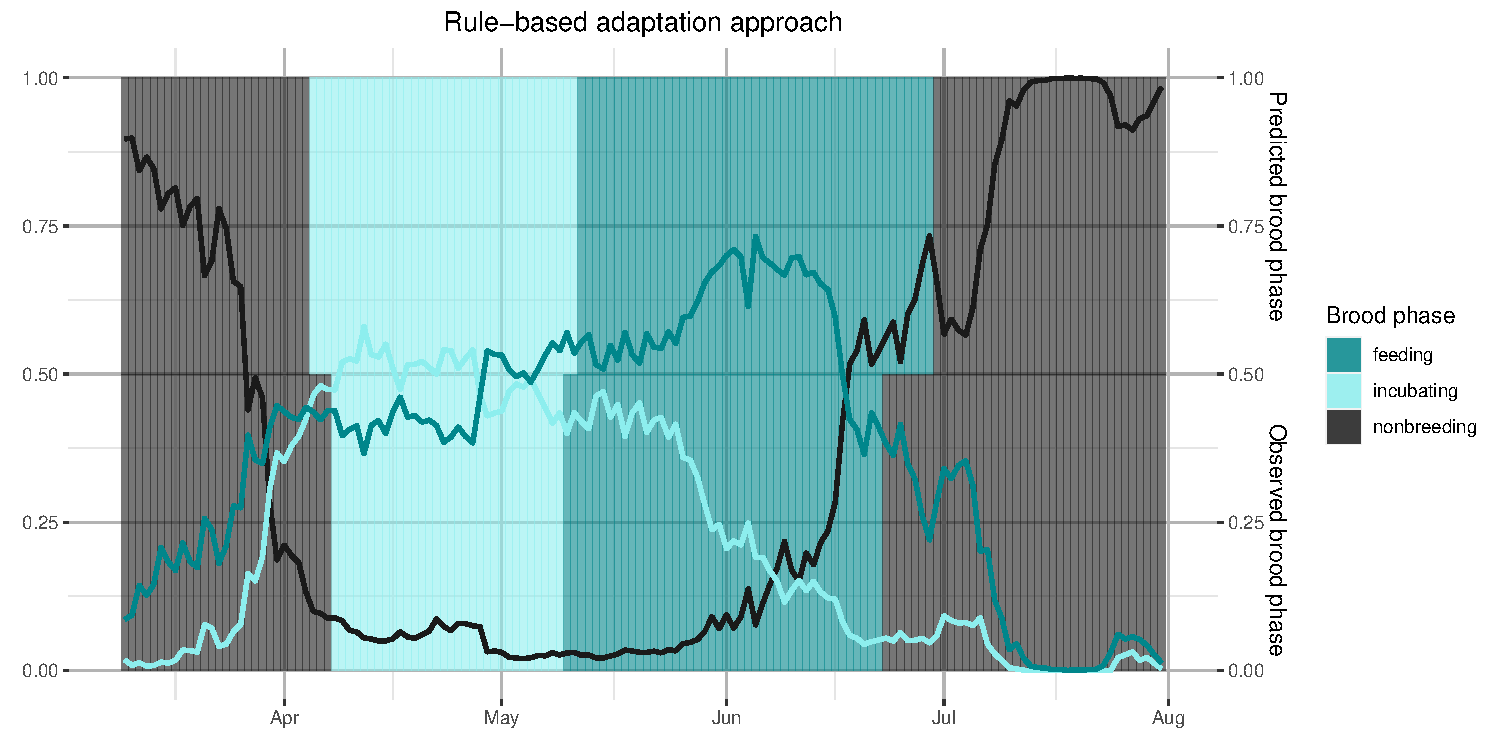
\includegraphics[width=0.54\textwidth]{figures/methods/08_prediction_example_rule.pdf}
\caption[Example of an MLRM prediction]{Example of the model predictions for an individual. The lines show the calculated probability for one of the three categories (light blue = incubating, turquoise = feeding, grey = non-breeding). The bars in the lower half of the plot show the actual breeding behaviour based on field observation data, while the bars in the upper half show the predicted category. The predictions based on the raw model prediction approach (left) are compared to the predictions based on the rule-based adaptation approach (right).}
\label{figure:example_prediction}
\end{figure}



\subsubsection{Validation of Brood Phase Identification}
Finally, the model was validated with two different datasets.

On the one hand, there were FP cases that remained after the two steps of home range detection (Section~\ref{subsection:homerange}) and nest detection (Section~\ref{subsection:nest}). These individuals were assigned a nest even though they did not breed at all. With the data of these individuals, the performance of the MLRM could be validated on non-breeding red kites. This step served to investigate whether the model reliably recognises non-breeding individuals as such and does not misinterpret their movement behaviour as breeding behaviour.

On the other hand, the model was applied to the movement data of the 28 successfully breeding adults in Thuringia provided by Thomas Pfeiffer. With the data of these individuals, the performance of the model could be validated on movement data from other geographical regions. This step served to investigate whether the scaling and centering of the variables allows a reliable application of the model to individuals with different scales of movement behaviour.

\newpage
\section{Results}
\subsection{Home Range Detection}
A total of 908 years of data stemming from 309 individuals met the requirements for conducting a home range detection. The validation data shows that out of these 908 cases, in 49\% (441) of all cases there was a settlement in a home range and in 51\% (467) of all cases there was no settlement in a home range.

After performing the home range detection, a home range was predicted for 69\% (626) of all cases. Based on the validation data, 429 out of these 626 actually had a home range, while 197 did not have a home range (Table~\ref{table:conf_matrix_hr}). Thus, 69\% (429 out of 626) of the positively predicted cases were correctly predicted. For 31\% (282) of all cases, no home range was predicted. Based on the validation data, 270 out of these 282 actually had no home range, while 12 did have a home range. Thus, 96\% (270 out of 282) of the negatively predicted cases were correctly predicted. Overall, 77\% (699 out of 908) of the cases could be correctly predicted, resulting in an accuracy of 77\%. While a value of 97\% was achieved for recall, the precision is 69\% and MCC is 60\% (Table~\ref{table:stats_hr_and_nest}).

\begin{table}[H]
\begin{center}
\caption[Confusion matrix of the home range detection result]{Confusion matrix of the home range detection result.}
\label{table:conf_matrix_hr}
\begin{tabularx}{0.5\textwidth} {
    | >{\centering\arraybackslash}X 
    | >{\centering\arraybackslash}X 
    | >{\centering\arraybackslash}X | }
\hline
Total \break = 908 & \textbf{Predicted \break positive} & \textbf{Predicted \break negative} \\
\hline
\textbf{Actually \break positive} &
\cellcolor[HTML]{CCFFCC} TP = 429 \break (47.3\%) & % green
\cellcolor[HTML]{FFCCCC} FN = 12 \break (1.3\%) \\  % red
\hline
\textbf{Actually \break negative} &
\cellcolor[HTML]{FFCCCC} FP = 197 \break (21.7\%) &  % red
\cellcolor[HTML]{CCFFCC} TN = 270 \break (29.7\%) \\ % green
\hline
\end{tabularx}
\end{center}
\end{table}

The differences between the two categories (whether a home range was occupied or not) and both sexes are shown in Figure~\ref{figure:hr_area_centroid_displacement_sex_diff}. The differences were analysed statistically using a t-test. With a p-value of < 2.2$\times10^{-16}$, the category with home range shows a significantly higher number of consecutive weeks spent in an area of less than 60 km$^2$ than the category without home range. There is also a difference between both sexes for the cases where a home range was present with a p-value of 0.02, indicating that male individuals tend to spend more consecutive weeks in an area of less than 60 km$^2$. Regarding the centroid displacement between the respective areas, a p-value of < 2.2$\times10^{-16}$ shows that the cases without a home range have a significantly higher centroid displacement than the cases with a home range. There is, however, no significant difference between the two sexes for cases where a home range was present is with a p-value of 0.48.

\begin{figure}[H]
\centering
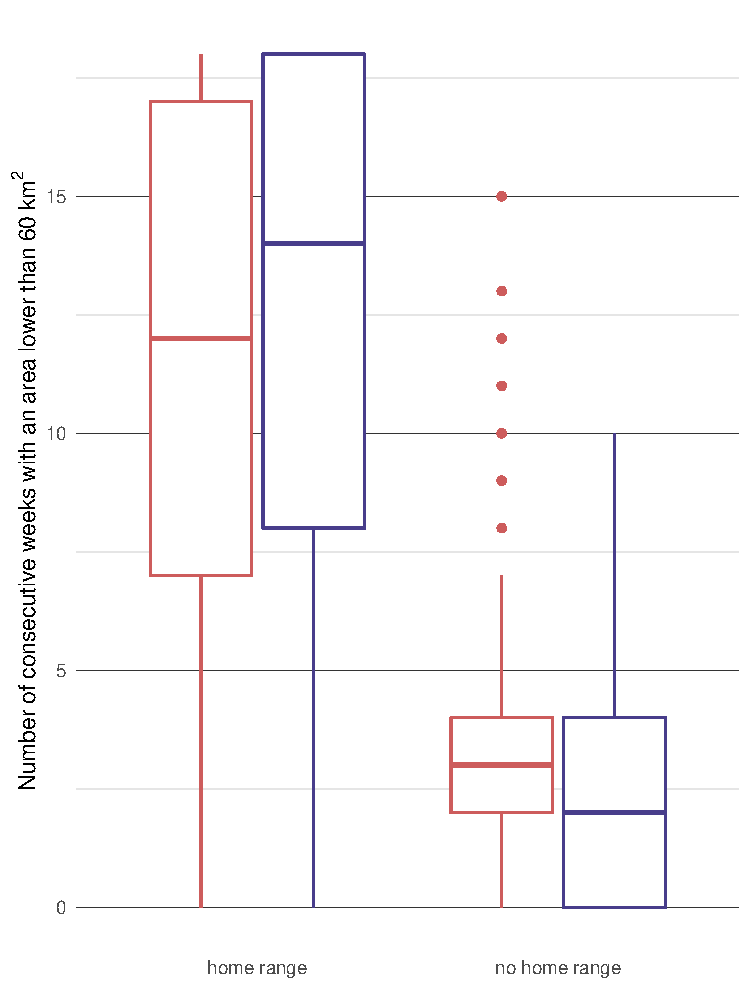
\includegraphics[width=0.4\textwidth]{figures/results/02_hr_area_sex_diff_no_legend.pdf}
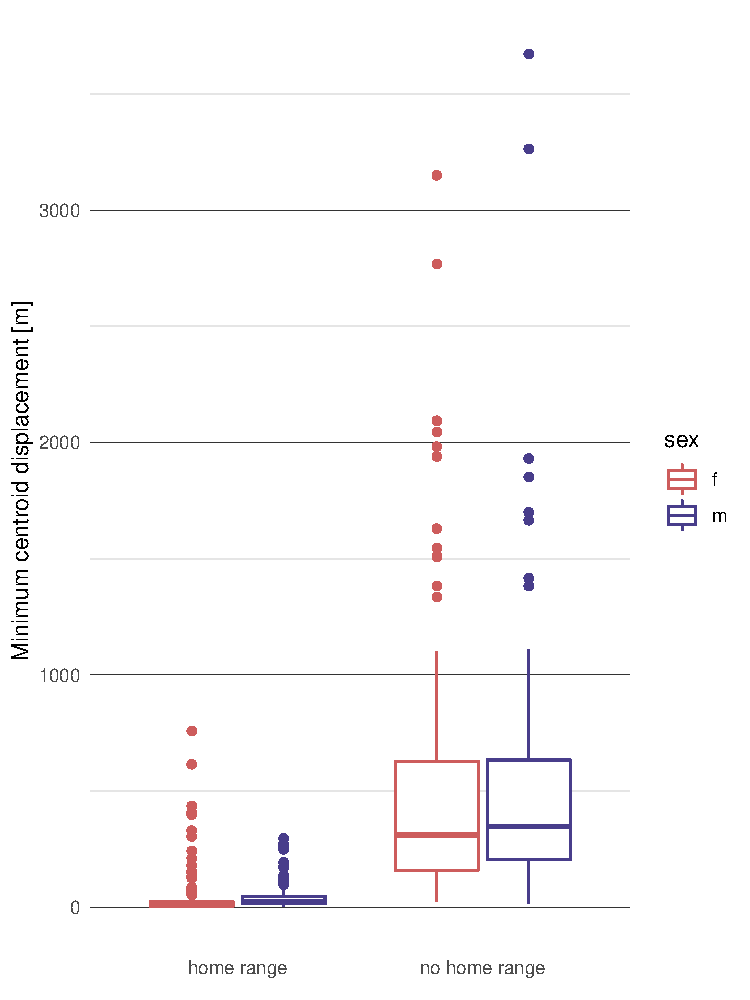
\includegraphics[width=0.4\textwidth]{figures/results/04_centroid_displacement_sex_diff.pdf}
\caption[Boxplot of birds with and without home range]{The boxplots show the difference in consecutive weeks with an area usage of < 60km$^2$ (left) and minimum centroid displacement between consecutive MCPs (right) for female (red) and male (blue) individuals with and without a home range according to the validation data.}
\label{figure:hr_area_centroid_displacement_sex_diff}
\end{figure} 


\subsection{Nest Detection}
The 626 positively predicted cases of the previous step were considered for nest detection analyses. Out of these 626 cases, 624 met the minimum data requirements to perform a nest detection analysis. The validation data shows that out of these 624 cases, in 58\% (365) of all cases a nest was occupied and in 42\% (259) of all cases no nest was detected in field observations.

After performing the nest detection, a nest was predicted for 70\% (437) of all cases. Based on the validation data, 364 out of these 437 actually had a nest, while 73 did not have a nest (Table \ref{table:conf_matrix_nest}). Thus, 83\% (364 out of 437) of the positively predicted cases were correctly predicted. For 31\% (187) of all cases, no nest was detected. Based on the validation data, 186 out of these 187 actually had no nest, while 1 did have a nest. Thus, 99\% (186 out of 187) of the negatively predicted cases were correctly predicted.  Overall, 88\% (550 out of 624) of the cases could be correctly predicted, resulting in an accuracy of 88\%. While a value of 99\% was achieved for recall, the precision is 83\% and MCC is 77\% (Table~\ref{table:stats_hr_and_nest}).

\begin{table}[H]
\begin{center}
\caption[Confusion matrix of the nest detection result]{Confusion matrix of the nest detection result.}
\label{table:conf_matrix_nest}
\begin{tabularx}{0.5\textwidth} {
    | >{\centering\arraybackslash}X 
    | >{\centering\arraybackslash}X 
    | >{\centering\arraybackslash}X | }
\hline
Total \break = 624 & \textbf{Predicted \break positive} & \textbf{Predicted \break negative} \\
\hline
\textbf{Actually \break positive} &
\cellcolor[HTML]{CCFFCC} TP = 364 \break (58.3\%) & % green
\cellcolor[HTML]{FFCCCC} FN = 1 \break (0.2\%) \\  % red
\hline
\textbf{Actually \break negative} &
\cellcolor[HTML]{FFCCCC} FP = 73 \break (11.7\%) &  % red
\cellcolor[HTML]{CCFFCC} TN = 186 \break (29.8\%) \\ % green
\hline
\end{tabularx}
\end{center}
\end{table}

The differences between the two categories (whether a nest was present or not) and both sexes are shown in Figure~\ref{figure:res_time_revisits_sex_diff}. The differences were analysed statistically using a t-test. With a p-value of < 2.2$\times10^{-16}$, the category with a nest shows a significantly higher mean daily residence time at the calculated nest location than the category without a nest. Also, the difference between the two sexes for cases where a nest was present is significantly higher with a p-value of < 2.2$\times10^{-16}$, indicating that female red kites tend to spend significantly more time at the nest. Regarding the mean daily revisitations to the calculated nest location, a p-value of < 2.2$\times10^{-16}$ shows that the cases with a nest have a significantly higher revisitation rate than the cases without a nest. The difference between the two sexes for cases where a nest was present is also significant with a p-value of < 2.2$\times10^{-16}$. Female individuals tend to revisit the calculated nest location significantly more than male individuals.

\begin{figure}[H]
\centering
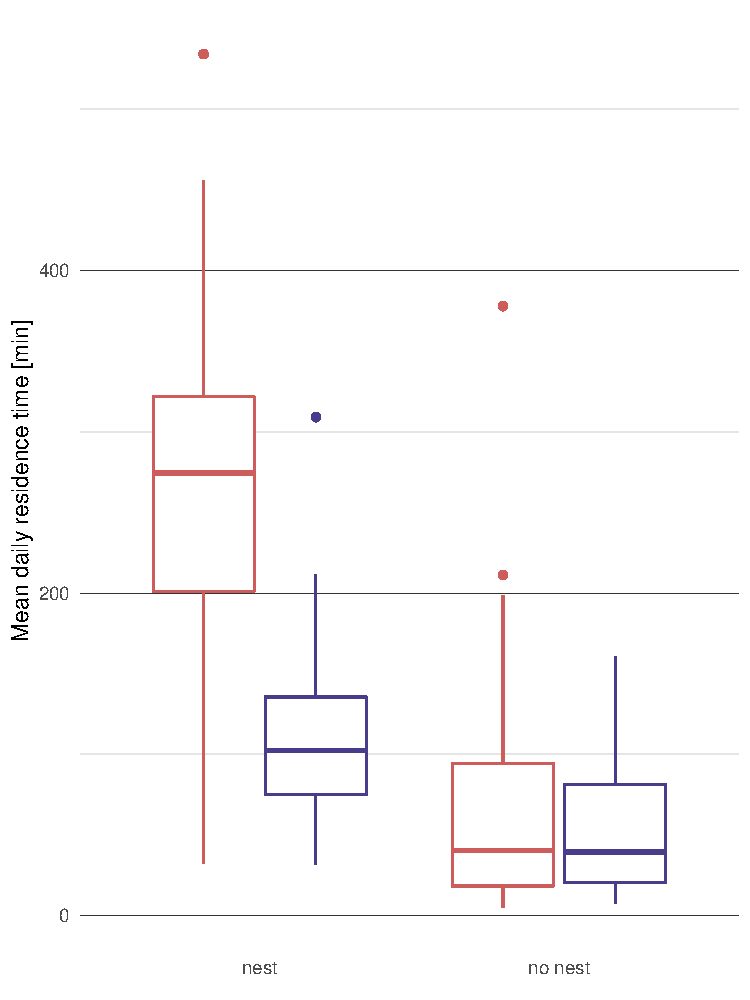
\includegraphics[width=0.4\textwidth]{figures/results/05_residence_time_sex_diff_no_legend.pdf}
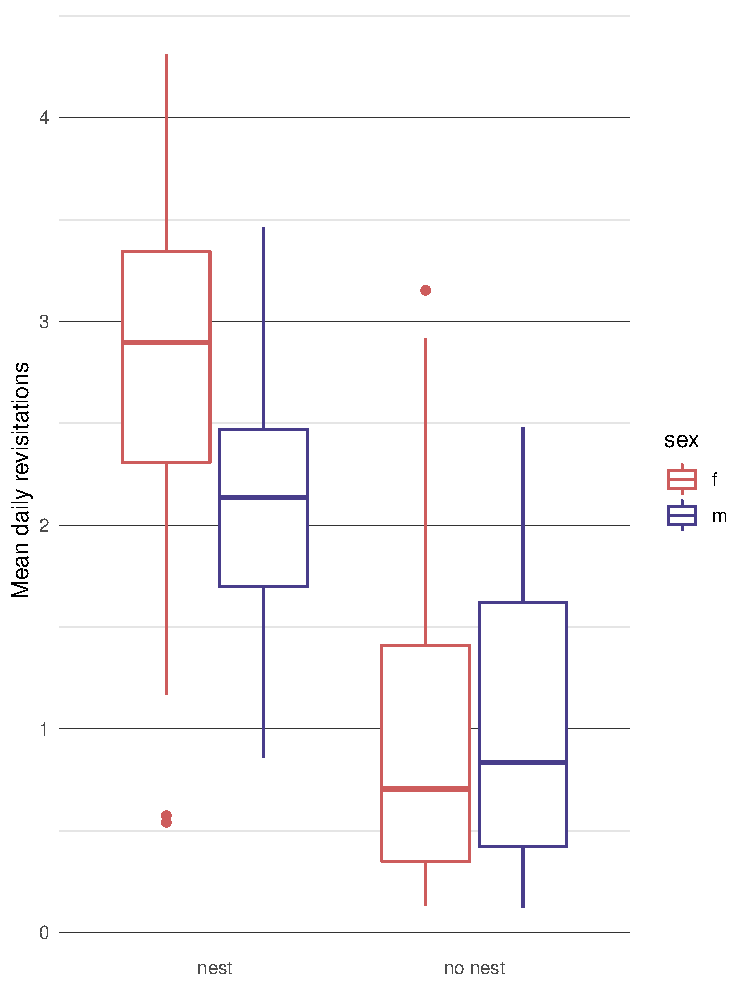
\includegraphics[width=0.4\textwidth]{figures/results/07_revisits_sex_diff.pdf}
\caption[Boxplot of birds with and without nest]{The boxplots show the difference in mean daily residence time (left) and mean daily revisitations (right) at the nest location for female (red) and male (blue) individuals with and without a nest according to the validation data.}
\label{figure:res_time_revisits_sex_diff}
\end{figure}

\vspace{1\baselineskip}

\begin{table}[H]
\begin{center}
\caption[Statistical metrics of the home range detection and the nest detection]{Overview of the statistical metrics of the home range detection and the nest detection.}
\label{table:stats_hr_and_nest}
\begin{tabular}{| p{3cm} | p{3cm} | p{3cm} |} 
\cline{1-3}
\textbf{Statistical \newline metric} & \textbf{Home Range \newline Detection} & \textbf{Nest Detection} \\
\hline
Accuracy & 77\% & 88\% \\ 
\hline
Recall & 97\% & 99\% \\
\hline
Precision & 69\% & 83\% \\
\hline
MCC & 60\% & 77\% \\
\hline
\end{tabular}
\end{center}
\end{table}



\newpage
\subsection{Accuracy of Nest Locations}
Of the 437 individuals for which a nest location was identified, for the 364 TP (the individuals that actually have a nest according to the validation data) the distance to the actual nest location was on average 71~m +/- 272~m with a median of 45~m. Of the 364 predicted nest locations, 361 were within a 1~km radius of the actual nest location. 99\% of all predicted nest locations were within a 784~m radius of the actual nest location, 95\% within a 119~m radius, and 50\% within a 34~m radius (Figure~\ref{figure:nest_dist_barplot}).

\begin{figure}[H]
\centering
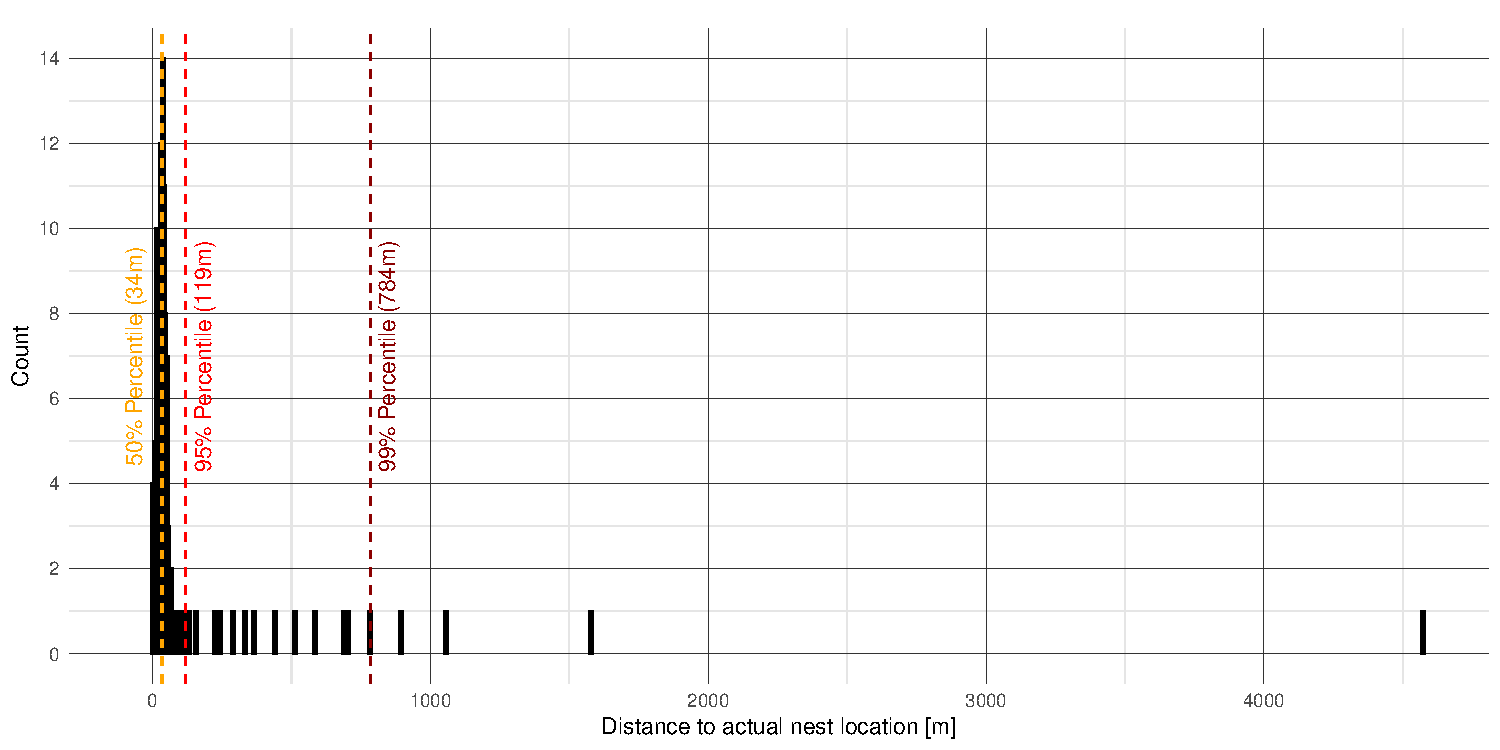
\includegraphics[width=1\textwidth]{figures/nest/nest_dist_bar.pdf}
\caption[Distances of the predicted nest locations from the actual nest locations]{Distribution of the distances of the 364 predicted nest locations from the actual nest locations.}
\label{figure:nest_dist_barplot}
\end{figure}

The distance of the predicted nest location to the actual nest location was also analysed with regard to the sex of the birds. Conducting a t-test shows with a p-value of 0.4809 that there is no significant difference between female and male individuals regarding the distance to the actual nest location.



\subsection{Brood Phase Identification}
The variable estimates of the MLRM were analysed for all three brood phases and are visualised in Figure~\ref{figure:variable_estimates} with the non-breeding phase as reference level. In the incubating phase the revisitations showed the strongest effect on the overall population, meaning that revisitations are higher during incubation compared to the non-breeding phase. Also the distance to the nest had a strong effect, decreasing during incubation. The 95\% MCP area of female individuals showed the strongest effect in the incubation phase, which decreases compared to male individuals. In the feeding phase revisitations and the 95\% MCP area increase compared to the non-breeding phase. For female individuals, the distance to the nest decreases and the residence time at the nest increases during feeding compared to male individuals. Revisitations are higher during incubating than during feeding, while the 95\% MCP area is larger during feeding than during incubating. Female individuals have a smaller 95\% MCP area usage, longer residence time at the nest and fewer revisitations at the nest location during incubating than during feeding.


\begin{figure}[H]
\centering
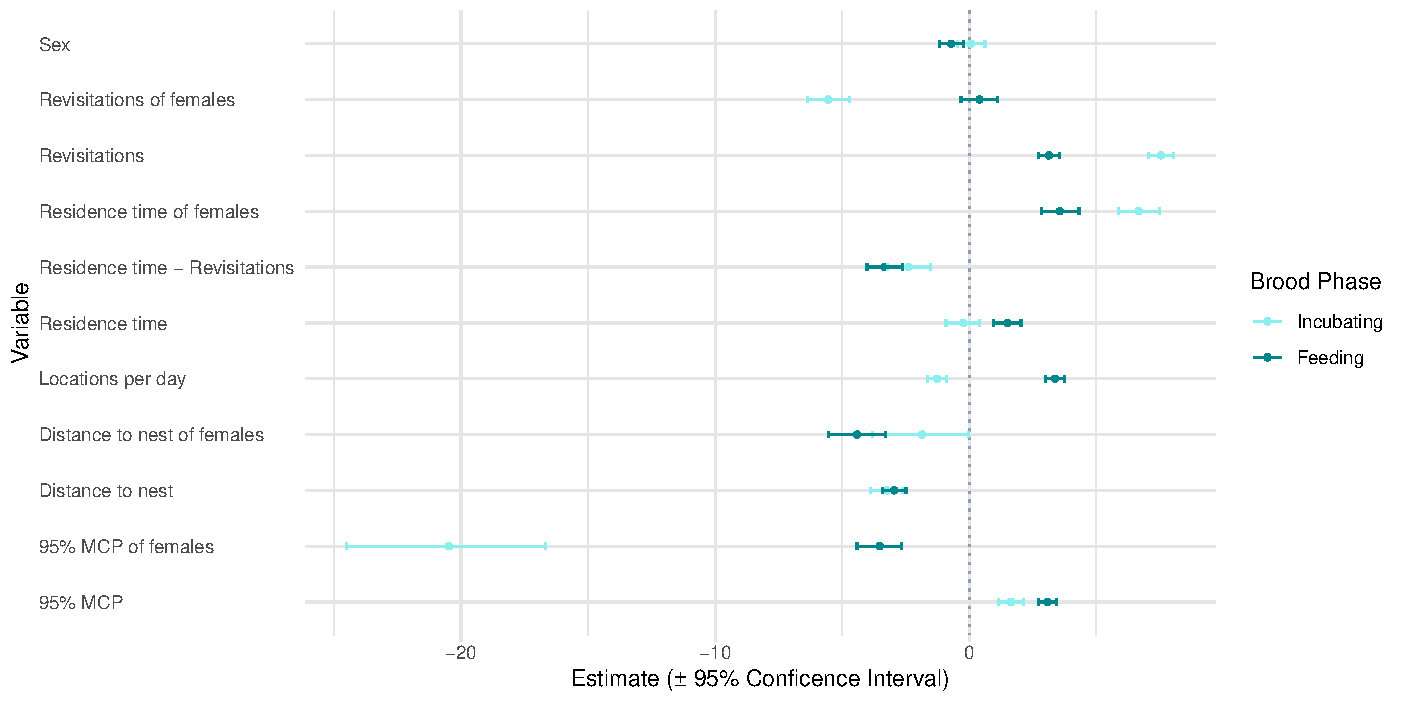
\includegraphics[width=1\textwidth]{figures/results/04_coefplot_bm_15_separated_combined.pdf}
\caption[Variable estimates of the MLRM]{Estimates of the variables used in the MLRM, shown for the two categories of incubating and feeding individuals, respectively, compared to the non-breeding category (represented as dotted line with value 0).}
\label{figure:variable_estimates}
\end{figure}


\subsubsection{Daily Predictions}
For the raw model predictions approach, 64\% of all days across all breeding cycles were correctly predicted. 49\% of all incubating days, 41\% of all feeding days and 84\% of all non-breeding days were correctly predicted. With this approach, an accuracy of 64\% was achieved. A value of 55\% was achieved for recall, 57\% for precision and 25\% for MCC (Table~\ref{table:stats_breeding_model}).

For the merged categories approach, 76\% of all days across all breeding cycles were correctly predicted. 73\% of all breeding days and 78\% of all non-breeding days were correctly predicted. With this approach, an accuracy of 76\% was achieved. A value of 73\% was achieved for recall, 78\% for precision and 51\% for MCC (Table~\ref{table:stats_breeding_model}).

For the rule-based adaptation approach, 69\% of all days across all breeding cycles were correctly predicted. 59\% of all incubating days, 46\% of all feeding days and 88\% of all non-breeding days were correctly predicted. With this approach, an accuracy of 69\% was achieved. A value of 57\% was achieved for recall, 71\% for precision and 38\% for MCC (Table~\ref{table:stats_breeding_model}).


\begin{table}[H]
\begin{center}
\caption[Statistical metrics of the different brood phase identification approaches]{Overview of the statistical metrics of the different brood phase identification approaches.}
\label{table:stats_breeding_model}
\begin{tabular}{| p{3cm} | p{3cm} | p{3cm} | p{3cm} | } 
\cline{1-4}
\textbf{Statistical \newline metric} & \textbf{Raw model \newline predictions} & \textbf{Merged \newline categories} & \textbf{Rule-based \newline adaptation} \\
\hline
Accuracy & 64\% & 76\% & 69\% \\ 
\hline
Recall & 55\% & 73\% & 57\% \\
\hline
Precision & 57\% & 78\% & 71\% \\
\hline
MCC & 25\% & 51\% & 38\% \\
\hline
\end{tabular}
\end{center}
\end{table}



\subsubsection{Brood Success Classification}
For the raw model predictions approach, 1.5\% (1 of 67) of all breeding cycles fulfill the criteria of a breeding bird, i.e. at least 28 days of incubation and 42 days of feeding of the nestlings.

For the merged categories approach, 39\% (26 of 67) of all breeding cycles fulfill the criteria of a breeding bird, i.e. at least 70 days of breeding.

For the rule-based adaptation approach, 8\% (5 of 67) of all breeding cycles fulfill the criteria of a breeding bird, i.e. at least 28 days of incubation and 42 days of feeding of the nestlings.



\subsubsection{Validation with Non-Breeding Red Kites}
Of the 73 FP cases that remained after nest detection, 34 cases had sufficient data to calculate the variables needed to apply the MLRM. Predictions of breeding behaviour were made for these 34 individuals.

For the raw model predictions approach, 48\% of all days across all breeding cycles were correctly predicted as non-breeding. 18\% (6 of 34) of all breeding cycles are falsely classified as breeding individuals.

For the merged categories approach, 41\% of all days across all breeding cycles were correctly predicted as non-breeding. 62\% (21 of 34) of all breeding cycles are falsely classified as breeding individuals.

For the rule-based adaptation approach, 56\% of all days across all breeding cycles were correctly predicted as non-breeding. 24\% (8 of 34) of all breeding cycles are falsely classified as breeding individuals.

The accuracy of the daily predictions is lower than for the breeding individuals. However, more breeding cycles are classified as successful in all classification methods.




\subsubsection{Validation with Red Kites in Thuringia}
The following results were obtained for the 28 successful broods of red kites in Thuringia:

For the raw model predictions approach, 51\% of all days across all breeding cycles were correctly predicted. 35\% of all incubating days, 65\% of all feeding days and 48\% of all non-breeding days were correctly predicted. With this approach, an accuracy of 51\% was achieved. A value of 79\% was achieved for recall, 45\% for precision and 11\% for MCC (Table~\ref{table:stats_breeding_model_pfeiffer}). 29\% (8 of 28) of all breeding cycles are correctly classified as breeding individuals.

For the merged categories approach, 72\% of all days across all breeding cycles were correctly predicted. 89\% of all breeding days and 45\% of all non-breeding days were correctly predicted. With this approach, an accuracy of 72\% was achieved. A value of 89\% was achieved for recall, 73\% for precision and 38\% for MCC (Table~\ref{table:stats_breeding_model_pfeiffer}). 86\% (24 of 28) of all breeding cycles are correctly classified as breeding individuals.

For the rule-based adaptation approach, 69\% of all days across all breeding cycles were correctly predicted. 65\% of all incubating days, 61\% of all feeding days and 79\% of all non-breeding days were correctly predicted. With this approach, an accuracy of 69\% was achieved. A value of 73\% was achieved for recall, 70\% for precision and 37\% for MCC (Table~\ref{table:stats_breeding_model}). 57\% (16 of 28) of all breeding cycles are correctly classified as breeding individuals.

The statistical metrics are similar to the breeding individuals in the Swiss data, slightly lower or higher depending on the classification method. However, more breeding cycles are classified as successful in all classification methods.

\begin{table}[H]
\begin{center}
\caption[Statistical metrics of the different brood phase identification approaches applied to red kites in Thuringia]{Overview of the statistical metrics of the different brood phase identification approaches applied to red kites in Thuringia.}
\label{table:stats_breeding_model_pfeiffer}
\begin{tabular}{| p{3cm} | p{3cm} | p{3cm} | p{3cm} | } 
\cline{1-4}
\textbf{Statistical \newline metric} & \textbf{Raw model \newline predictions} & \textbf{Merged \newline categories} & \textbf{Rule-based \newline adaptation} \\
\hline
Accuracy & 51\% & 72\% & 69\% \\
\hline
Recall & 79\% & 89\% & 73\% \\
\hline
Precision & 45\% & 73\% & 70\% \\
\hline
MCC & 11\% & 38\% & 37\% \\
\hline
\end{tabular}
\end{center}
\end{table}

\newpage
\section{Discussion}
This study showed that GPS movement data of red kites can be successfully used to analyse different aspects of the breeding cycle. With an accuracy of 77\%, it could be reliably determined whether an individual occupies a home range. In a further step, nest locations of red kites could be reliably localised with an accuracy of 88\%. For breeding birds, depending on the approach, it was possible to correctly predict whether an individual was breeding in up to 76\% of the days. However, a reliable classification of whether a breeding cycle was successful or not could not be achieved.

\subsection{Home Range Detection}
With an accuracy of 77\%, the overall proportion of correctly predicted cases is high. The high recall of 97\% is achieved by the fact that only 2.7\% (12 of 441 cases) of home ranges remained undetected. The precision of 69\% and the MCC of 60\% result from the relatively high proportion of FP with 21.7\%. The threshold values can be chosen differently in order to achieve a decreasing proportion of FP, which in turn leads to an increasing proportion of FN. This part of the algorithm is very flexible and can be adapted according to the purpose of its application.

The data of the 12 FN cases were inspected in order to further evaluate the performance of the method. It was found that in all cases the individuals did not have a nest and occupied a home range later in the summer. For the detection of the home range, only data during the months of February, March, April and May were considered. If data later in the year had been included, there would have been a risk of including movement data of birds after breeding. Later in the year, after breeding, there are birds that settle in a different place than the nest location and become stationary at communal roosting sites \parencite{spatz2022sex}. These behaviour patterns would be falsely identified by the algorithm as settlements in a home range. Later data could be of interest, especially considering that subadult individuals can settle temporarily in summer and autumn but do not breed yet. These temporary settlement areas are likely to be chosen as home range to start a breeding attempt in the spring of the following year \parencite{aebischer2021rotmilan}. These home ranges are ultimately also captured by the algorithm, as data from several years are analysed. Should it be of interest to specifically investigate cases of subadult settlements, the developed home range detection approach can be applied to subadult individuals by adjusting the time span of the input data.

The generated parameters are suitable for detecting a possible settlement in a home range, as the categories of cases with home range and without home range differ significantly both in the number of consecutive weeks with an area of less than 60~km$^2$ as well as in the distance of the centroid displacement (Figure~\ref{figure:hr_area_centroid_displacement_sex_diff}). Despite the significant differences in both parameters between the two categories (individuals with or without a home range), there was a high proportion of cases where a home range was falsely detected (FP). This is due to the fact that the main requirement was to miss as few settlements as possible. The increased proportion of FP was preferred over a higher rate of FN, as many of these cases can be filtered out in the later nest detection step.

An interesting finding is that the sex of the individuals has an influence on the number of consecutive weeks with an area of less than 60~km$^2$, where female red kites show a mean of 11.4 weeks compared to males with a mean of 12.6 weeks. Male red kites with a home range tend not to expand their area for a longer duration than female red kites. This behaviour could be due to the females expanding their home range as soon as they increase their contribution to the food supply for the nestlings, which happens when the nestlings are two to three weeks old \parencite{aebischer2021rotmilan}. For red kites breeding in western Switzerland, this moment is about 13-14 weeks after the start of nest building \parencite{scherler2023brutbiologie}. The expansion of the home range can be explained by the increasing food requirements of the nestlings \parencite{bischofberger2019werden, spatz2019raumnutzung}. The finding that females expand their home range towards the end of chick rearing and even exceed the values of the males is consistent with the findings of \textcite{spatz2019raumnutzung} and \textcite{spatz2021zwischen}. Apart from the fact that the sample size was small, \textcite{spatz2019raumnutzung} also emphasise the influence of brood loss, which in their study led to a shift in the home range area of females in particular. The reason why females occupy a home range of less than 60~km$^2$ for a significantly shorter duration than males cannot be conclusively explained. The potential influence of brood loss on the home range area was not analysed in this work. The fact that sex has no influence on the extent of the centroid displacement was to be expected given that the nest, as a fixed location, represents the focal point of the whole breeding cycle.



\subsection{Nest Detection}
With an accuracy of 88\%, the overall proportion of correctly predicted cases is high. The high recall of 99\% is achieved by the fact that only 1 out of 365 cases was falsely predicted to not have a nest. The precision (83\%) and the MCC (77\%) are slightly lower due to the fact that 11.7\% of the predicted cases were classified as FP. All statistical metrics have high values, indicating that nests can be reliably detected based on developed approach.

The data of the single false negative was inspected in order to further evaluate the performance
of the method. It was recognised that in this case there was too little data, which occurred too early in the year, so that the movement at the nest location was not emphasised enough. 

Both revisitations and residence time are suitable for detecting a possible nest location, as the categories of cases with a nest and without a nest differ significantly both in the mean daily revisitations as well as in the mean daily residence time (Figure~\ref{figure:res_time_revisits_sex_diff}). Despite the significant differences in both parameters between the two categories (individuals with or without a nest), there was a considerable proportion of cases where a nest was falsely detected (FP). A better separation was not possible as the focus was on detecting all nests and thus keeping the FN as small as possible while still aiming for an optimal separation of both categories. Should it be of interest to produce as little FP as possible at the cost of missing actual nests, the limit values of the mean daily revisitations and the mean daily residence time can be manually increased.

For red kites with a nest, there are significant differences between the sexes in both residence time at the nest and revisitation of the nest. On the one hand, it is obvious that females have a higher residence time at the nest, as the female takes care of incubation while the male provides food. On the other hand, the fact that revisitations are also higher for females than for males may seem counterintuitive. However, there are many occasions where the female leaves the nest for a short time and then returns. This may be to copulate, to defend the nest or to receive food from the male \parencite{aebischer2021rotmilan}. As the male is foraging most of the time and thus away from the nest location, fewer GPS locations are located at the nest, which consequently leads to a lower revisitation rate. The pattern may also be due to the fact that data were taken into account from February onwards, where the female was not yet breeding and the pair was preparing the nest.

For the nest detection method, limited prior knowledge of the species and the data structure regarding the revisitation rate and the residence time at the nest site must be available, but a seasonal restriction, as required in \textit{nestR}, is not needed. Furthermore, the nest detection method is based on recursive movement patterns, which is computationally more efficient than the Bayesian hierarchical model used in \textit{nestR}.



\subsection{Accuracy of Nest Locations}
The predicted nest locations correspond well with the actual locations according to the validation data (Figure \ref{figure:nest_dist_barplot}). With 95\% of all cases, most predicted nest locations are located within a radius of less than 120~m from the actual nest, which shows that the region of the nest can already reliably be localised.

The predicted nests with a distance of more than one kilometre to the actual nest location were all female individuals with an unsuccessful brood. The furthest distance of the predicted nest location to the actual nest location of a female with a successful brood is 243~m. For a male with a successful brood the furthest distance is 894~m.

The inaccuracies in locating the nest locations may be due to the fact that the brood history of the individuals was not taken into account. However, there were also cases where individuals built a nest but never got to breed. There were also cases of brood losses where individuals moved away from the nest after the loss and did not return to it. In these cases, the time in which the individuals showed a recursive movement pattern was limited, which made the detection of the nest difficult.

Statistically, there is no significant sex-specific difference in the performance of the detection of the nest location. It is interesting to see that nest locations of females and males can be determined with equal accuracy, especially considering the different movement patterns, which are most pronounced during the incubation phase. It appears that the nest site is the centre of attention for both females and males during the entire incubation period, which is clearly visible in the movement patterns. It can be concluded that there is no need for separate approaches for the detection of the nest site for both sexes.



\subsection{Brood Phase Identification}
\subsubsection{Daily Predictions}
The performance of the MLRM applied on the test dataset shows that for 64\% of the days it can be correctly predicted whether an individual has been incubating, feeding or non-breeding, while with 88\% the highest accuracy was achieved for non-breeding days. It can be concluded from this that the phase in which no breeding takes place can be very reliably separated from breeding phase. The other metrics (recall, precision and MCC) do not indicate an excellent performance. In addition, it was concluded from the low accuracy values for the categories incubating (49\%) and feeding (41\%) that they are hard to separate from each other. Therefore, another approach was to combine the two categories into the category breeding. This resulted in a high accuracy both overall (76\%) and for the two categories breeding (73\%) and non-breeding (78\%), while all other statistical metrics were also higher than with the raw model predictions approach. This has shown that GPS movement data can be successfully used to distinguish breeding days from non-breeding days.

As it would be desirable to predict the categories incubating and feeding separately, the third approach of rule-based adaptation was developed. This was intended to fill gaps where possible missing data or weather influences had affected the analysed movement patterns to such an extent that the actual behaviour could not be identified. This approach improved the predictions slightly compared to the raw model predictions. Different rule sets were developed and applied, some of which performed better, which was clearly due to over-manipulating of the predictions. It is a challenge to define rules that adjust incorrect predictions while not manually over-adjusting the predictions to meet the expectations. In this work, no rule set could be elaborated that improved the predictions considerably.

The performance of the algorithm is poor when applied to non-breeding individuals. All three approaches achieved similar predictions with an accuracy range of 41-56\%, which equals a random prediction. The fact that many days were classified as incubating or feeding shows that the behaviour of non-breeding individuals is partly comparable to that of breeding individuals, which can be explained by the fact that non-breeding individuals, especially young ones, often stay at common roosting sites that are revisited like a nest site \parencite{aebischer2021rotmilan}. The fact that this behaviour is misinterpreted in the predictions of the MLRM is not problematic, if the pattern of incubating and feeding days (Appendix~\ref{appendix:mlrm_predictions_nonbreeding}) could be detected by later classification and interpreted as a non-breeding individual.

When applied to the successfully breeding red kites in Thuringia, the performance of the algorithm was similar to the test dataset. The accuracies showed similar values, although not the non-breeding days showed the highest accuracies, but the breeding and feeding days. This was most evident in the merged categories approach, where 89\% of all breeding days were detected as such. Due to the different geographical regions and the associated different movement patterns, which are most evident in larger home ranges, this is a remarkable result, as it implies that the algorithm can be successfully applied to other geographical regions with different characteristics. An analysis of the performance of the home range and nest detection method on red kites in other geographical regions was not realised this work.

\subsubsection{Brood Success Classification}
The classification of predictions from the MLRM into successful and unsuccessful broods showed the best results when the merged categories approach was used as a basis. For the test dataset, 39\% of the cases were correctly classified as successful broods. For the red kites in Thuringia, even 86\% of the cases were correctly classified as successful broods. This result shows that the MLRM provides a good foundation for detecting successful broods. For the non-breeding individuals, 64\% of the cases were incorrectly classified as successful broods, which clearly shows the weaknesses of the approach of classifying the broods into successful and unsuccessful. However, this is not a weakness of the MLRM, but rather a weakness of the classification method, as the sum of days per category was added up. Considering that GPS telemetry-based datasets often show data gaps of one or several days, missing days can occur during the incubating or feeding phase. If the days of the respective category are added up, this number can be lower than the actual number of days. Therefore, an approach that considers the duration of the phases as a time span rather than the sum of all days might be more promising.

When the predictions of the MLRM are analysed visually, a rough pattern of a brood cycle corresponding to the expected pattern can be recognised for many cases from the predictions for the test dataset (Appendix~\ref{appendix:mlrm_predictions_test}) and the predictions for the individuals from Thuringia (Appendix~\ref{appendix:mlrm_predictions_thuringia}). In most cases, incubating days accumulate at the beginning of the breeding cycle, while feeding days accumulate in the end of the breeding phase. Overall, a brood can often be guessed from the pattern. For the non-breeding individuals, on the other hand, the plots show either much more noise or sections of only one of the categories incubating or feeding, resulting in no clear patterns (Appendix~\ref{appendix:mlrm_predictions_nonbreeding}). This implies that the predictions should be dividable into successful and unsuccessful broods based on the noise ratio in the predictions. 



\subsection{Research Objective}
An algorithm to quantify the breeding phenology of red kites was successfully developed, by implementing a set of suitable parameters to detect breeding-specific movement patterns. In a first step, it can be determined whether an individual has settled in a home range. In a second step, it can be determined whether it has a nest and where it is located. On a daily basis, it can then be successfully predicted whether an individual is incubating, feeding or non-breeding. Only for the final classification of whether an individual had a successful brood or not, no reliable solution could be found. The application of the algorithm for the daily prediction of breeding behaviour to red kites in Thuringia has proven the suitability of the algorithm for regions with different landscape characteristics and thus different movement patterns of red kites. The first two steps of the algorithm, home range detection and nest detection, could also be suitable for use in other geographical regions, as the thresholds of the metrics can easily be adapted to fit the movement behaviour of the population under study. In summary, the research objective was largely achieved, even if the final step of brood success could not be optimised to the desired extent. All sub-steps of the algorithm were successfully implemented and provided valuable insights in the breeding behaviour of red kites.

\newpage
\section{Conclusion}
\subsection{Major Findings}
Technological advances and the resulting increasing availability of large samples of GPS movement data enabled the development of the algorithm presented in this work.

An algorithm was created that enables the analysis of the red kite's breeding cycle in several steps. In one run, for an individual or an entire cohort, the home range can be detected, the nest can be localized, and the breeding behaviour can be characterised on a daily basis. The modularity of the algorithm allows the analysis of individual aspects of the breeding cycle separately, which enables a broad range of applications. For the home range detection and nest detection steps, the thresholds are adjustable to suit the movement dimensions of the subpopulation under study. The algorithm for the analysis of the brood cycle, which produces day-by-day predictions for the respective brood phase, has the advantage that no prior knowledge of the extent of the movement patterns of the subpopulation under study is necessary, as the variables are all scaled and centred.

Predicting brood phases based on GPS movement data allows the brood cycles of several red kites to be studied remotely. This can help to significantly reduce the personnel and time required for field work and can generate valuable insights into the breeding behaviour of red kites, helping to better understand population dynamics and optimise conservation strategies. This can be helpful if monitoring on site is logistically not feasible, or if breeding behaviour is to be analysed on a large scale, for example with the LIFE EUROKITE dataset \parencite{lifeeurokiteproject}, which contains red kite movement data across Europe.

\subsection{Limitations}
In the two steps of home range and nest detection, prior knowledge of the population under study is required to set thresholds in order to obtain reasonable results. Although it can be assumed in ornithological research that this prior knowledge is available in most cases, it would be a simplification of the process if data could be analysed without parameterisation of the algorithm and the thresholds were set automatically on the basis of the movement data.

Many more variants of an MLRM could have been created and compared to find an optimised model. For example, the variables could have been weighted according to their estimates to increase the significance of the predictions. Also in the selection of variables, many more variables could have been tested, which would have resulted in a different performance of the model. A different parameterisation of the MLRM could possibly lead to better results.

Despite the good performance of the MLRM, it was not possible to develop an approach that could reliably interpret the duration of the two brood phases and conclude the brood success from them. A classification based solely on a deterministic approach does not seem to allow a reliable determination of brood success.

To enable the applicability of the algorithm to a broad number of datasets, this work was carried out with GPS movement data with a temporal resolution of one hour. However, fine-scale movement patterns may not be captured with this coarse resolution. The performance of the algorithm could possibly be improved by using data with a finer temporal resolution. However, this would increase the computational effort. It should also be noted that the higher resolution leads to higher spatio-temporal autocorrelation, which complicates the calculation of home ranges. Ultimately, such high-resolution data are rarer than data with a temporal resolution of one hour.

\subsection{Future Research}
In further steps, a more reliable classification of the model predictions into successful and unsuccessful broods would certainly be necessary. Instead of a deterministic approach based solely on biological rules, a probabilistic approach could achieve better results. Since the predictions are already calculated in probabilities, it would be optimal to derive further classification attempts of the individual days from these probabilities, instead of assigning the day to the category that achieves the highest probability. Another point that could improve the performance of the brood success classification would be an approach that determines the duration of each phase instead of the sum of its days. This could lead to better results especially because the duration of the phases was mostly underestimated by the approach presented in this work.
Improved interpretability of MLRM predictions could also lead to a more reliable definition of the timing of each brood phase. Breeding-relevant events such as egg laying or hatching could then be derived from this. With an improved classification method, even brood losses could be detected.
It would also be interesting to analyse the applicability of the algorithm to other species that show similar breeding behaviour. It may be possible to identify how the algorithm can be parameterised differently and gain insights into the effects of certain movement-specific variables on certain species.

These gains in knowledge about the remote interpretation of breeding behaviour allow the analysis of broods of numerous individuals even from areas that are difficult to access. This in turn contributes to the adaptation of conservation measures in order to protect endangered species.

\newpage
\printbibliography[title = Literature, heading = bibintoc]

\newpage
\section*{R Packages}
\addcontentsline{toc}{section}{R packages}
\renewcommand{\thesubsection}{\Alph{subsection}}
The following R packages were used in this work:
\begin{itemize}
    \item \textit{amt}, version 0.1.7
    \item \textit{brms}, version 2.18.0
    \item \textit{dplyr}, version 1.0.10
    \item \textit{ggplot2}, version 3.3.6
    \item \textit{recurse}, version 1.1.2
    \item \textit{sf}, version 1.0-8
\end{itemize}

\newpage
\section*{Appendix}
\addcontentsline{toc}{section}{Appendix}
\renewcommand{\thesubsection}{\Alph{subsection}}
\appendix \subsection{Summary of the Multinomial Logistic Regression Model} \label{appendix:mlrm_formula}
Family: categorical \newline
Data: Training dataset (Number of observations: 19973 days of 67 brood cycles) \newline
Draws: 4 chains, each with iter = 2000; warmup = 1000; thin = 1; total post-warmup draws = 4000 \newline
Formula:
\begin{align*}
BroodPhase = Sex + 95MCP^2 + MeanNestDistance + ResidenceTime + Revisitations \\
+ Sex x (95MCP^2 + MeanNestDistance + ResidenceTime + Revisitations) \\
+ ResidenceTime x Revisitations + nDailyLocations + (1 | YearID)
\end{align*}

\vspace{1\baselineskip}

\noindent Group-Level Effects: YearID (Number of levels: 155)

\begin{table}[H]
\footnotesize{
\begin{center}
\begin{tabular}{| p{5.3cm} | p{1.1cm} | p{1.1cm} | p{0.85cm} | p{0.95cm} | p{0.5cm} | p{1.3cm} | p{1.2cm} |} 
\hline
& \textbf{Estimate} & \textbf{Est.Error} & \textbf{l-95\%} & \textbf{u-95\%} & \textbf{Rhat} & \textbf{Bulk\_ESS} & \textbf{Tail\_ESS} \\
\hline
sd(Incubating\_Intercept) & 1.02 & 0.07 & 0.89 & 1.17 & 1.01 & 980 & 1750 \\ 
\hline
sd(Feeding\_Intercept) & 1.00 & 0.07 & 0.88 & 1.14 & 1.00 & 905 & 1781 \\
\hline
\end{tabular}
\end{center}
}
\end{table}


\noindent Population-Level Effects:

\begin{table}[H]
\footnotesize{
\begin{center}
\begin{tabular}{| p{5.3cm} | p{1.1cm} | p{1.1cm} | p{0.85cm} | p{0.95cm} | p{0.5cm} | p{1.3cm} | p{1.2cm} |}
\hline
& \textbf{Estimate} & \textbf{Est.Error} & \textbf{l-95\%} & \textbf{u-95\%} & \textbf{Rhat} & \textbf{Bulk\_ESS} & \textbf{Tail\_ESS} \\
\hline
\footnotesize{Incubating\_Intercept} & -1.40 & 0.23 & -1.86 & -0.95 & 1.00 & 1147 & 1968 \\ 
\hline
\footnotesize{Incubating\_Sex(f)} & 0.06 & 0.27 & -0.47 & 0.62 & 1.00 & 892 & 1356 \\ 
\hline
\footnotesize{Incubating\_95MCP} & 1.64 & 0.25 & 1.14 & 2.13 & 1.00 & 2157 & 2724 \\ 
\hline
\footnotesize{Incubating\_MeanNestDistance} & -3.24 & 0.32 & -3.89 & -2.61 & 1.00 & 1711 & 2591 \\ 
\hline
\footnotesize{Incubating\_ResidenceTime} & -0.24 & 0.34 & -0.92 & 0.40 & 1.00 & 2898 & 2634 \\ 
\hline
\footnotesize{Incubating\_Revisitations} & 7.54 & 0.26 & 7.04 & 8.05 & 1.00 & 2492 & 3103 \\ 
\hline
\footnotesize{Incubating\_nDailyLocations} & -1.26 & 0.19 & -1.63 & -0.89 & 1.00 & 3922 & 3097 \\ 
\hline
\footnotesize{Incubating\_Sex(f):95MCP} & -20.47 & 1.98 & -24.50 & -16.69 & 1.00 & 3299 & 2699 \\ 
\hline
\footnotesize{Incubating\_Sex(f):MeanNestDistance} & -1.86 & 0.98 & -3.82 & -0.02 & 1.00 & 1923 & 2678 \\ 
\hline
\footnotesize{Incubating\_Sex(f):ResidenceTime} & 6.66 & 0.40 & 5.88 & 7.49 & 1.00 & 1922 & 2714 \\ 
\hline
\footnotesize{Incubating\_Sex(f):Revisitations} & -5.55 & 0.42 & -6.38 & -4.72 & 1.00 & 1739 & 2397 \\ 
\hline
\footnotesize{Incubating\_ResidenceTime:Revisitations} & -2.39 & 0.42 & -3.20 & -1.54 & 1.00 & 3026 & 2925 \\ 
\hline
\footnotesize{Feeding\_Intercept} & -3.21 & 0.22 & -3.63 & -2.77 & 1.01 & 617 & 1758 \\
\hline
\footnotesize{Feeding\_Sex(f)} & -0.71 & 0.24 & -1.18 & -0.24 & 1.00 & 489 & 1212 \\ 
\hline
\footnotesize{Feeding\_95MCP} & 3.07 & 0.18 & 2.73 & 3.42 & 1.00 & 2005 & 2376 \\ 
\hline
\footnotesize{Feeding\_MeanNestDistance} & -2.95 & 0.24 & -3.42 & -2.49 & 1.00 & 1618 & 2604 \\ 
\hline
\footnotesize{Feeding\_ResidenceTime} & 1.50 & 0.28 & 0.94 & 2.03 & 1.00 & 2716 & 2874 \\ 
\hline
\footnotesize{Feeding\_Revisitations} & 3.12 & 0.22 & 2.71 & 3.56 & 1.00 & 2258 & 3098 \\ 
\hline
\footnotesize{Feeding\_nDailyLocations} & 3.37 & 0.19 & 3.01 & 3.75 & 1.00 & 4274 & 3239 \\ 
\hline
\footnotesize{Feeding\_Sex(f):95MCP} & -3.52 & 0.45 & -4.42 & -2.67 & 1.00 & 1726 & 2649 \\ 
\hline
\footnotesize{Feeding\_Sex(f):MeanNestDistance} & -4.41 & 0.56 & -5.55 & -3.31 & 1.00 & 1313 & 2065 \\ 
\hline
\footnotesize{Feeding\_Sex(f):ResidenceTime} & 3.56 & 0.37 & 2.82 & 4.31 & 1.00 & 1991 & 2650 \\ 
\hline
\footnotesize{Feeding\_Sex(f):Revisitations} & 0.40 & 0.37 & -0.32 & 1.12 & 1.00 & 1743 & 2646 \\ 
\hline
\footnotesize{Feeding\_ResidenceTime:Revisitations} & -3.34 & 0.36 & -4.03 & -2.62 & 1.00 & 3117 & 3267 \\ 
\hline
\end{tabular}
\end{center}
}
\end{table}



\newpage
\subsection{Raw Model Predictions for the Test Dataset} \label{appendix:mlrm_predictions_test}
\begin{figure}[H]
\centering
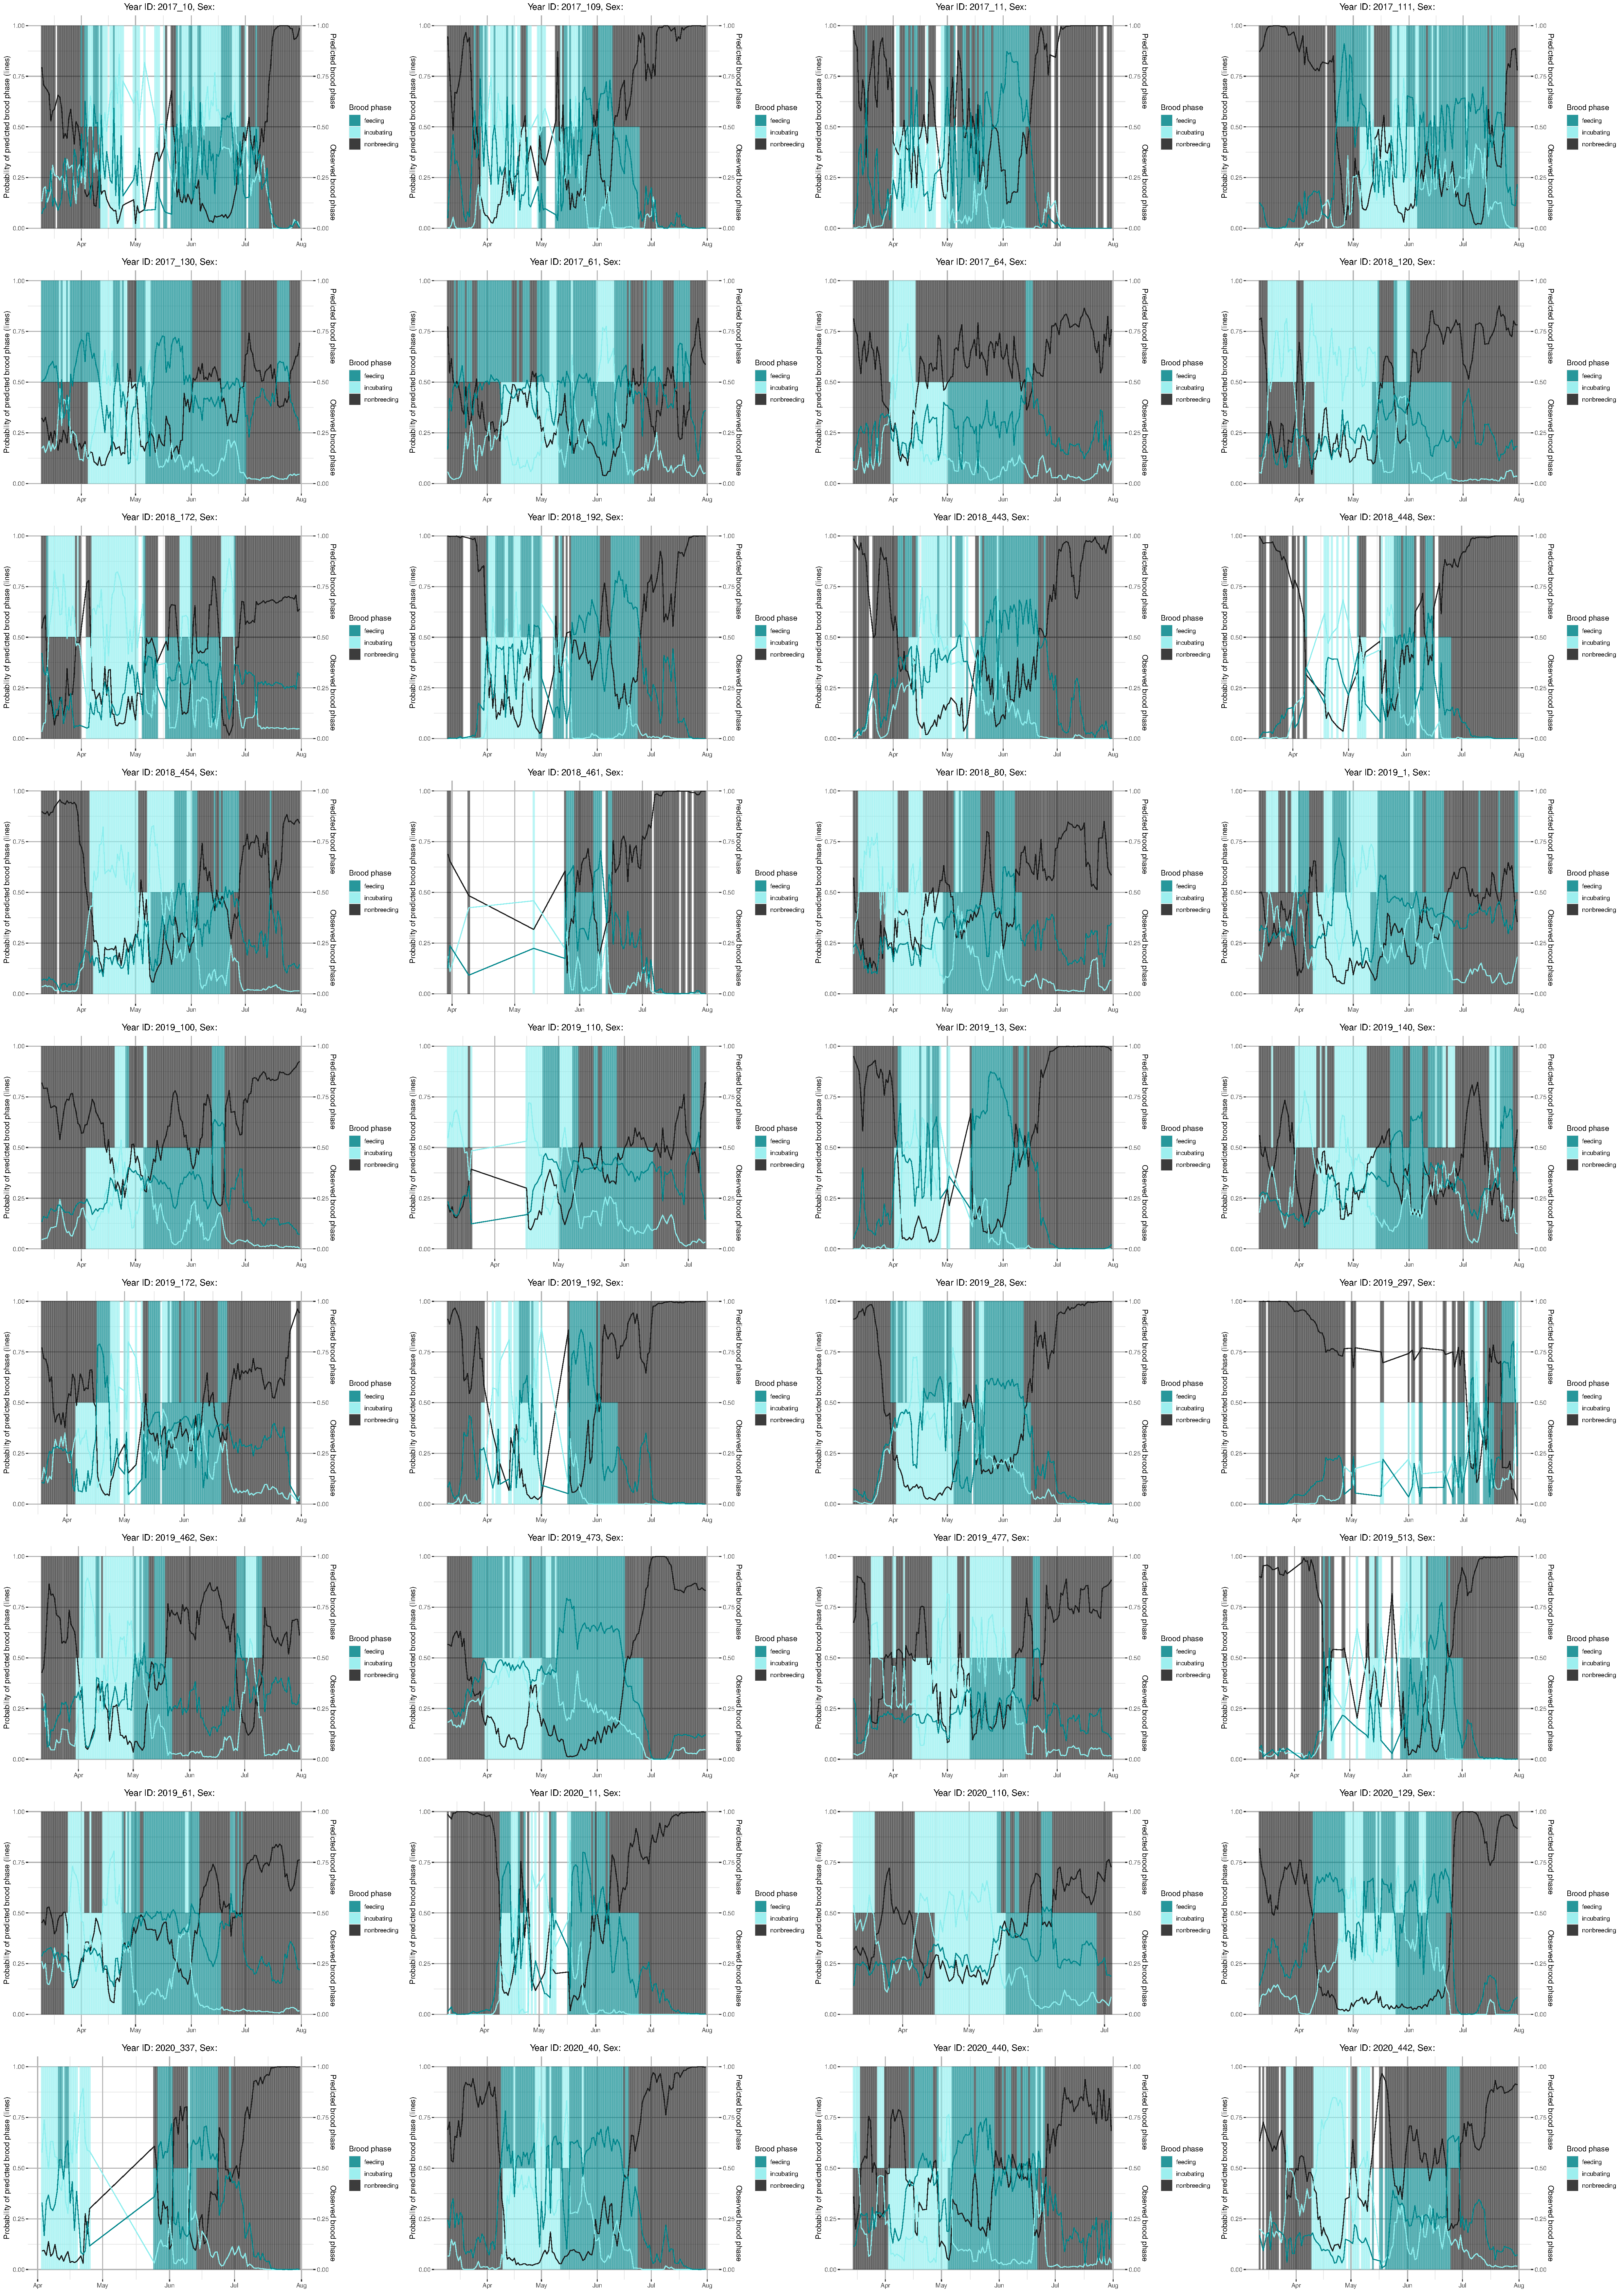
\includegraphics[width=1\textwidth]{figures/appendix/01_predictions_test_data_a.pdf}
\end{figure}
\newpage
\begin{figure}[H]
\centering
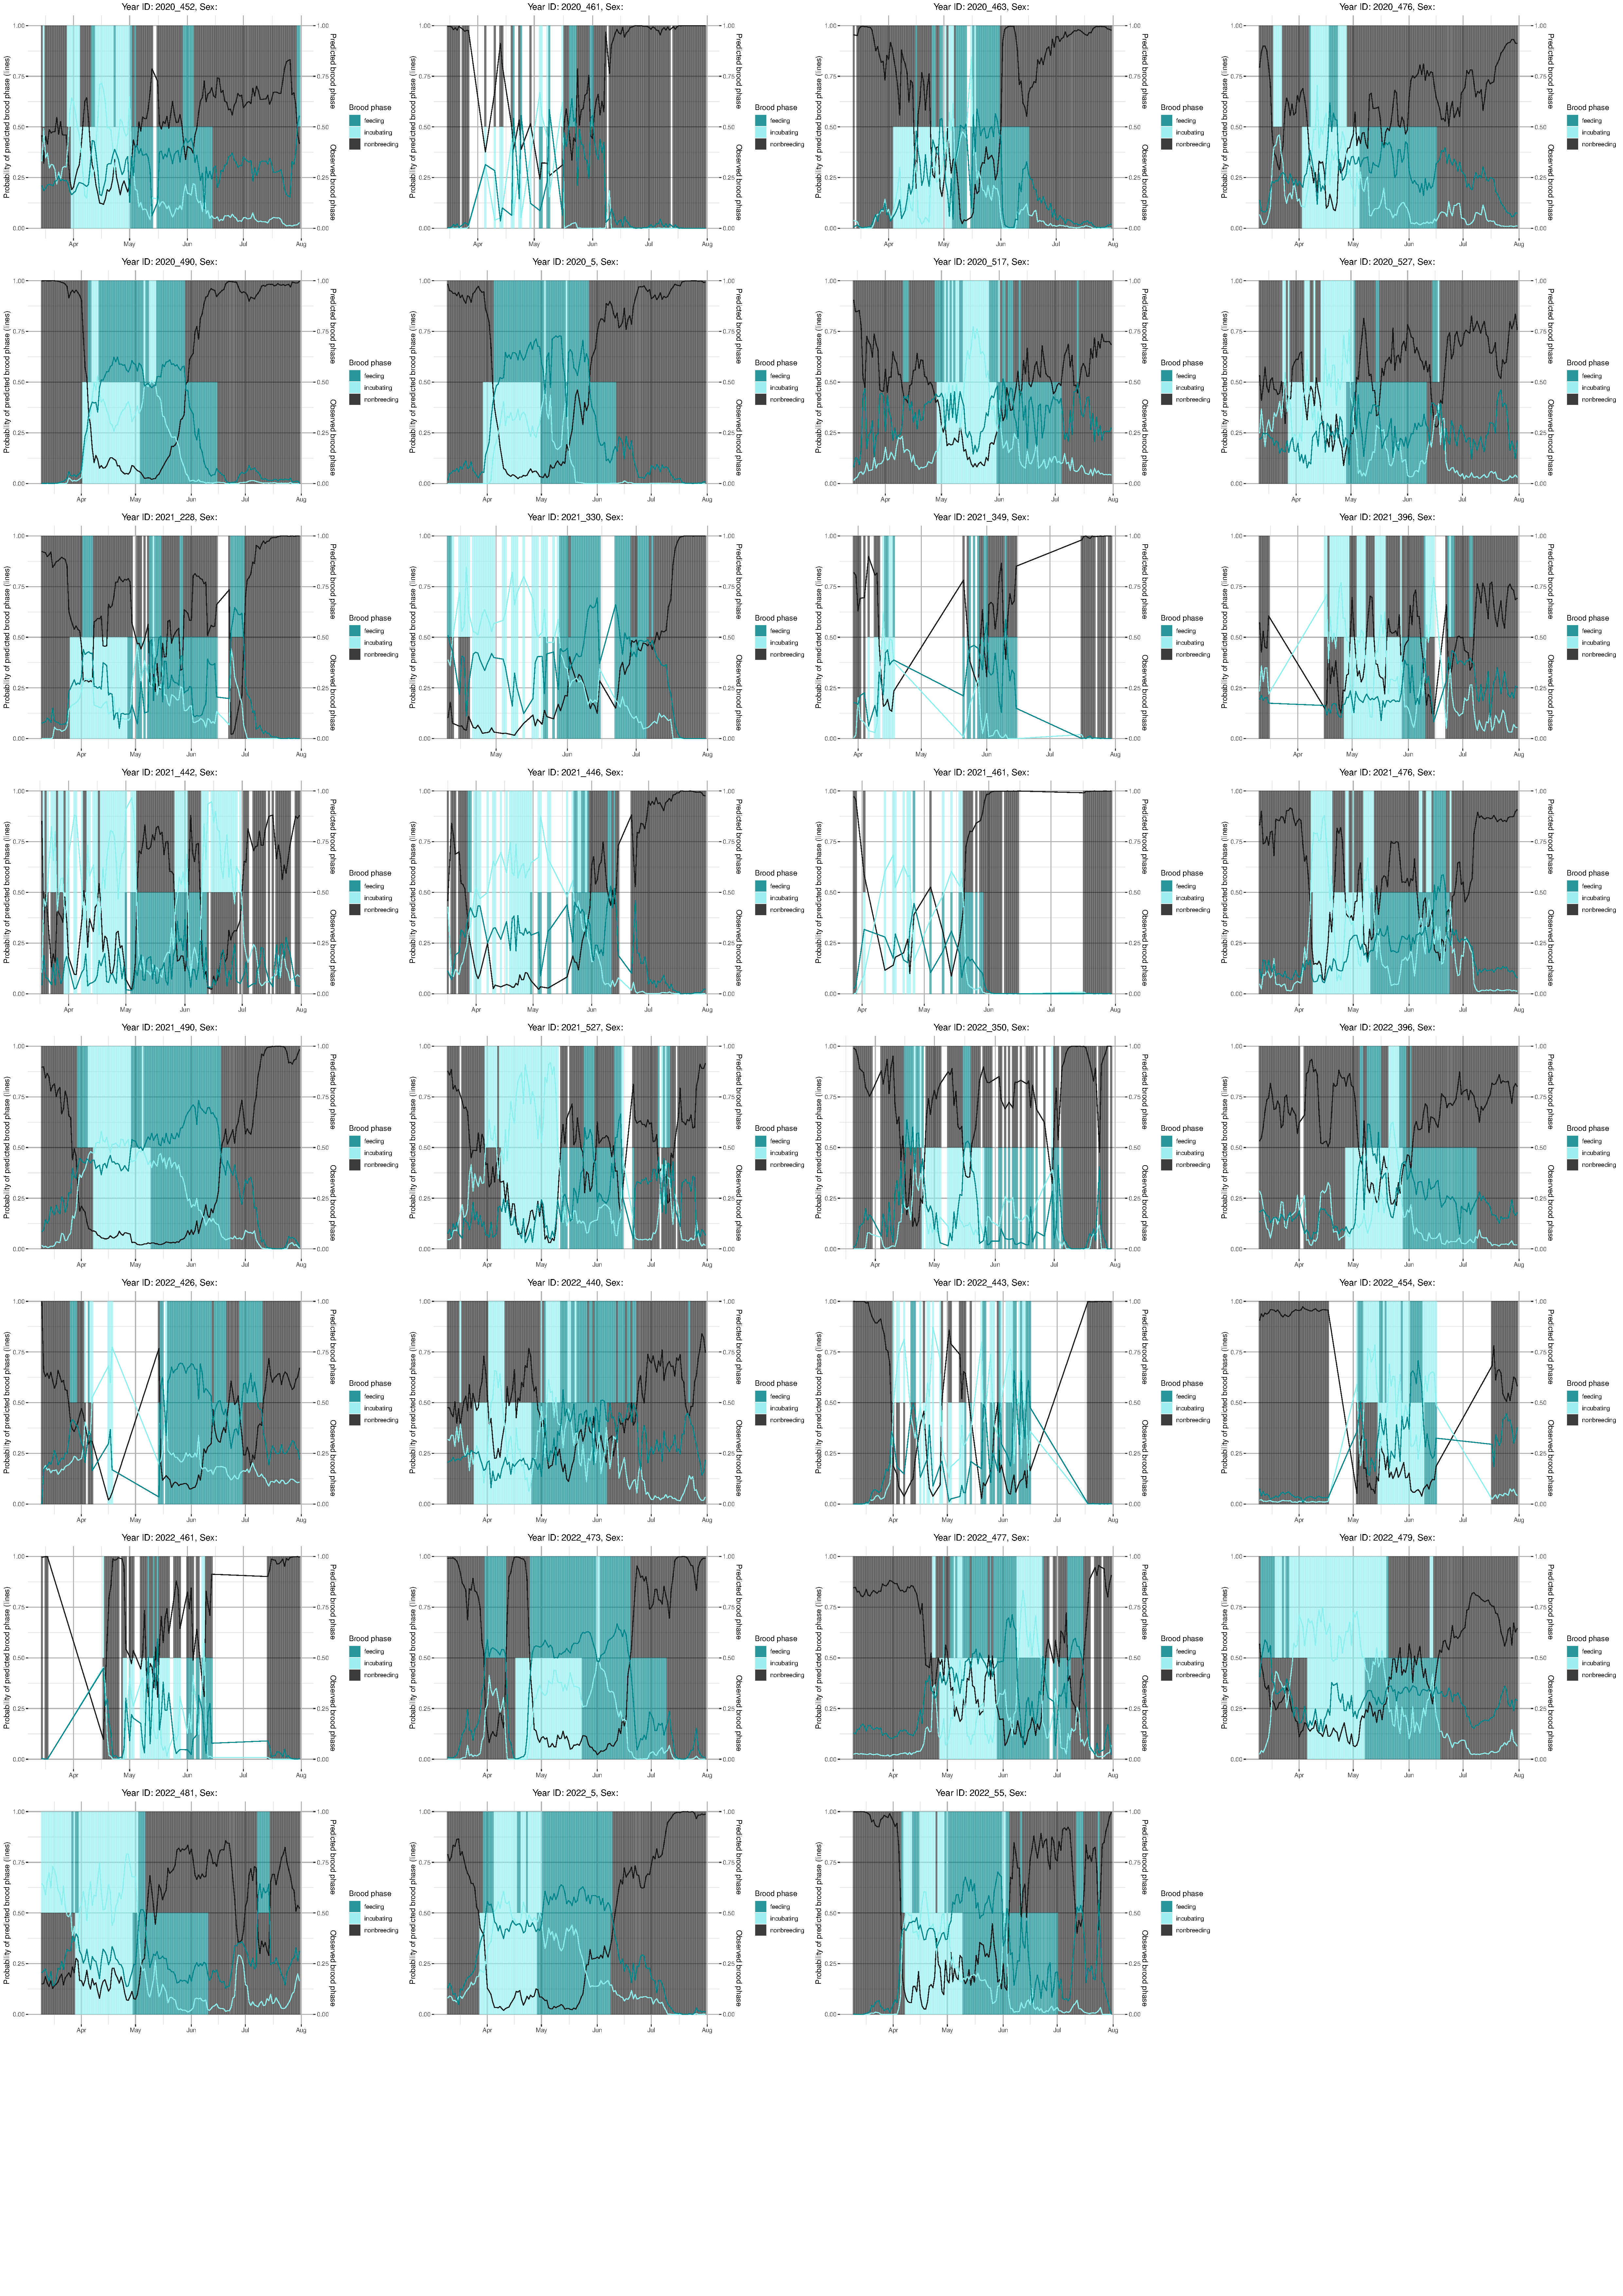
\includegraphics[width=1\textwidth]{figures/appendix/02_predictions_test_data_b.pdf}
\end{figure}



\newpage
\subsection{Raw Model Predictions for Non-Breeding Red Kites} \label{appendix:mlrm_predictions_nonbreeding}
\begin{figure}[H]
\centering
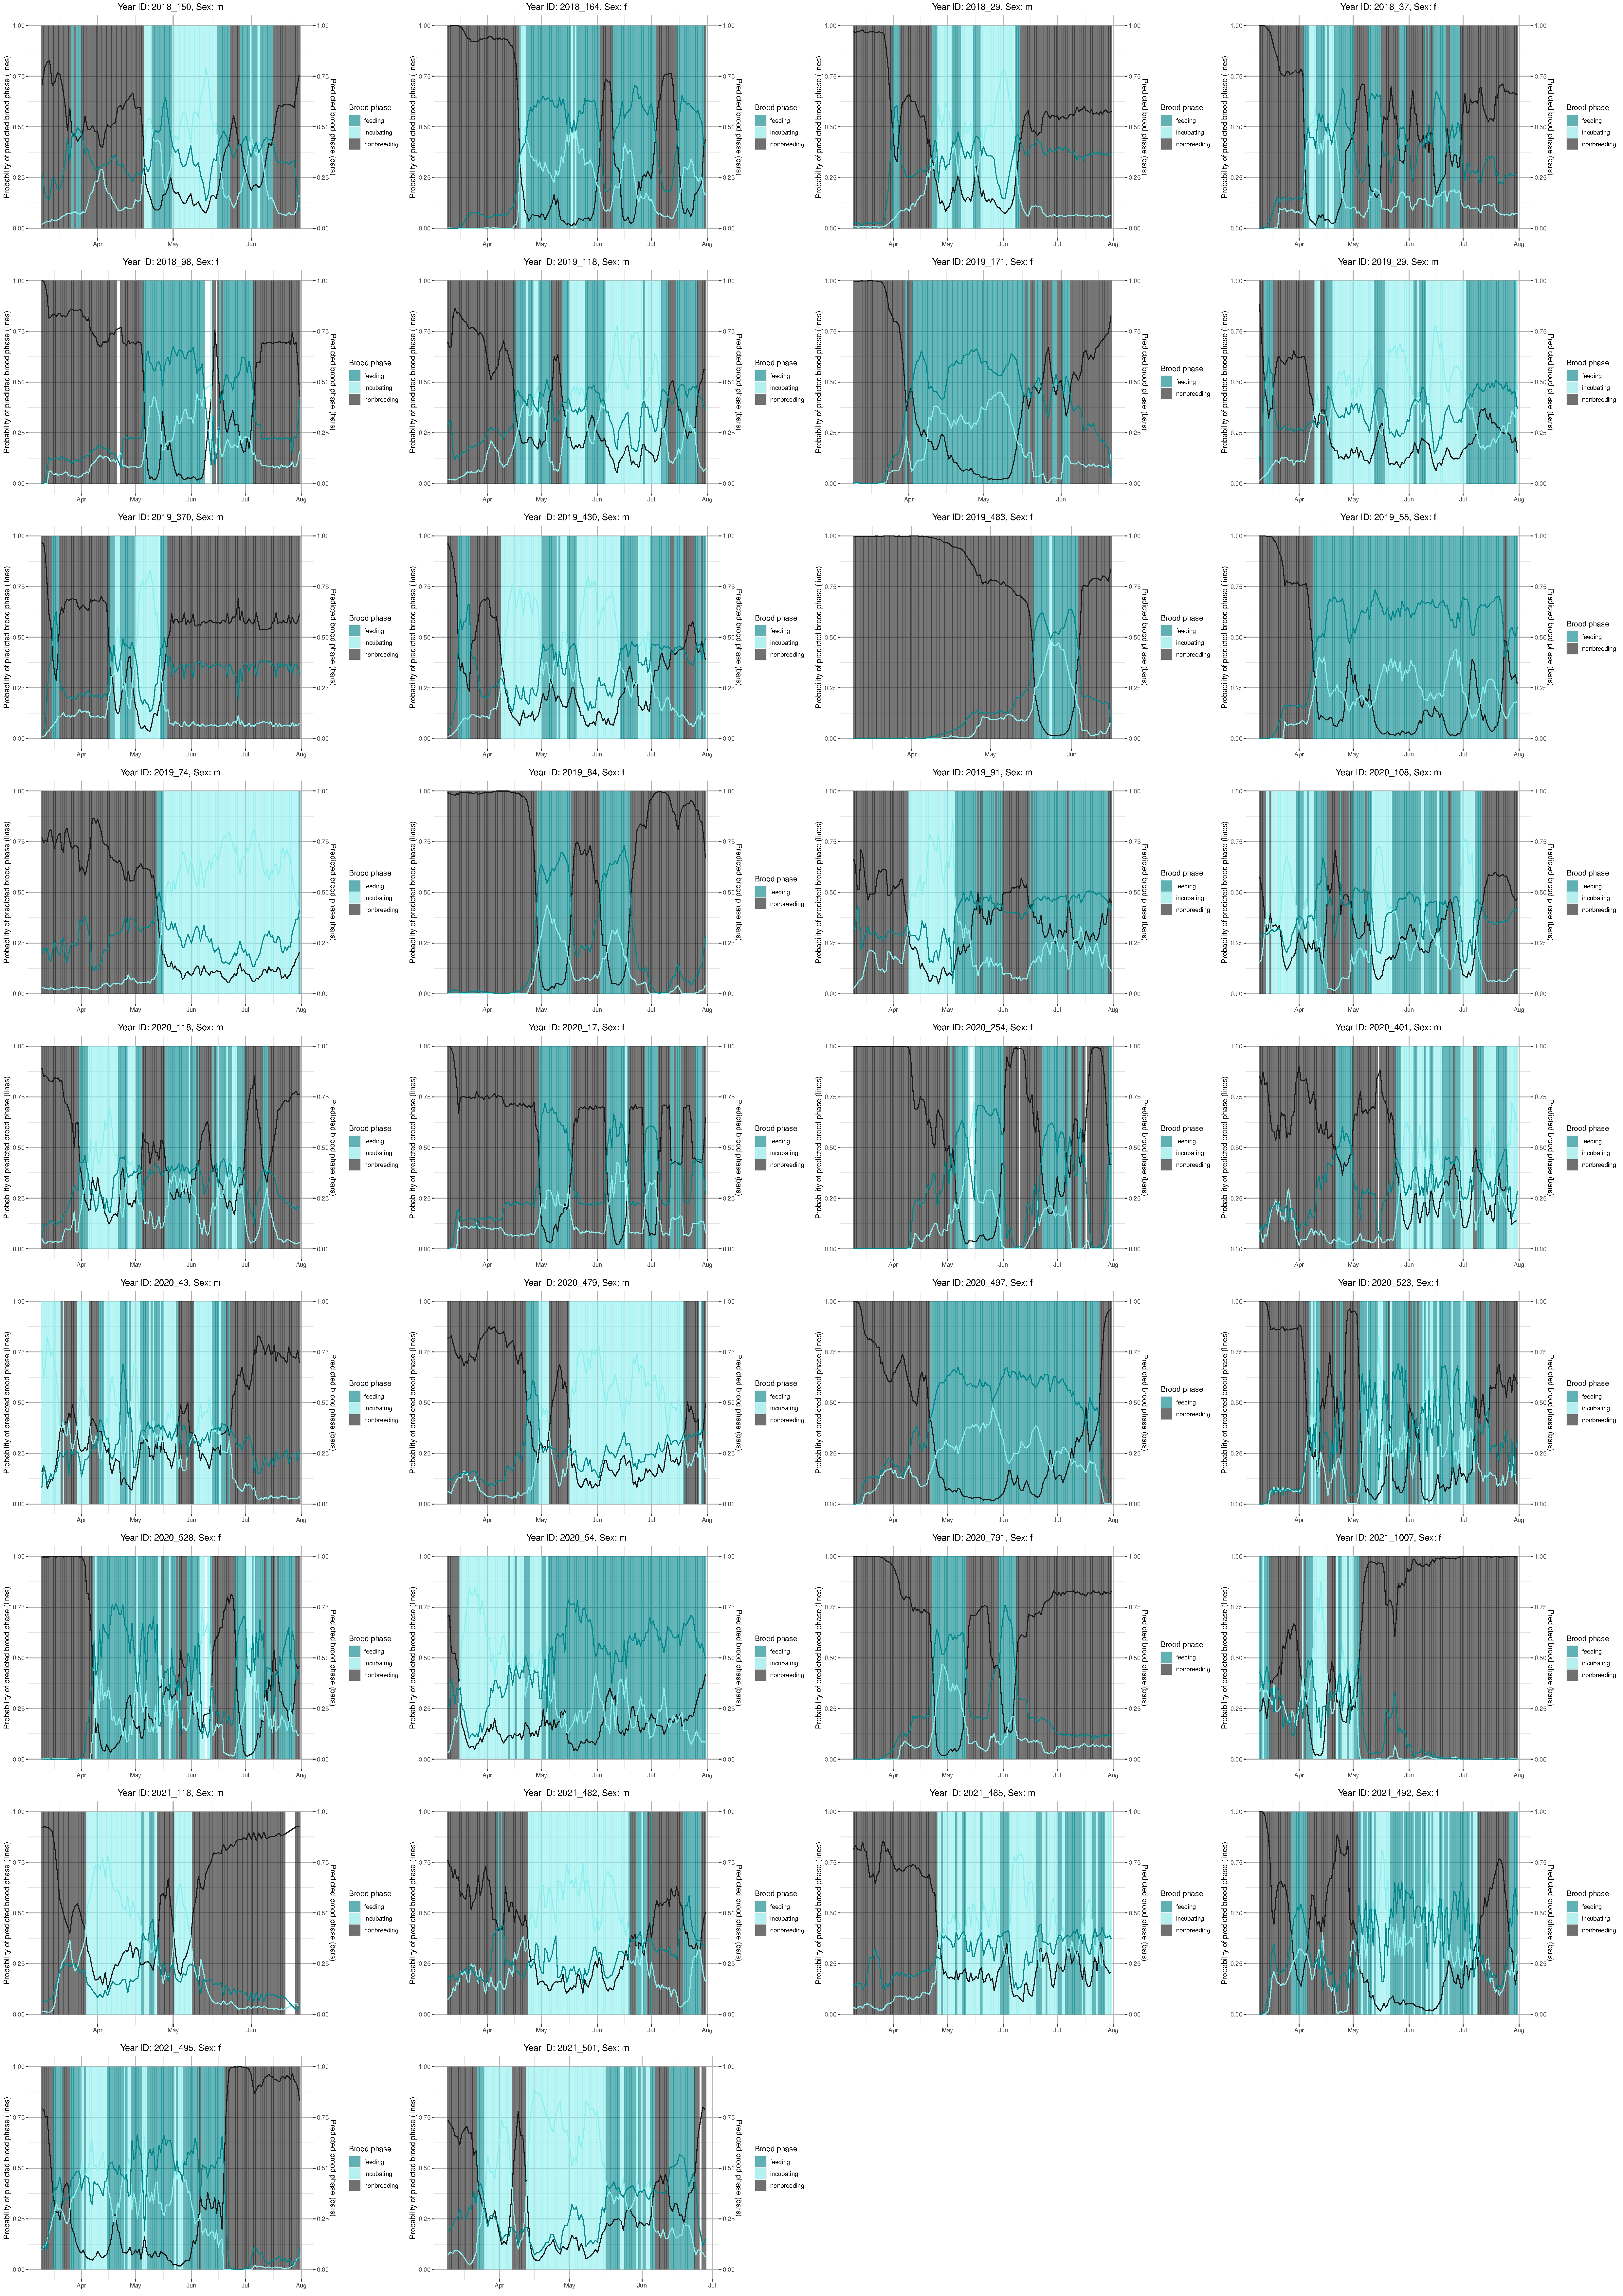
\includegraphics[width=1\textwidth]{figures/appendix/03_predictions_nonbreeders.pdf}
\end{figure}



\newpage
\subsection{Raw Model Predictions for Red Kites in Thuringia} \label{appendix:mlrm_predictions_thuringia}
\begin{figure}[H]
\centering
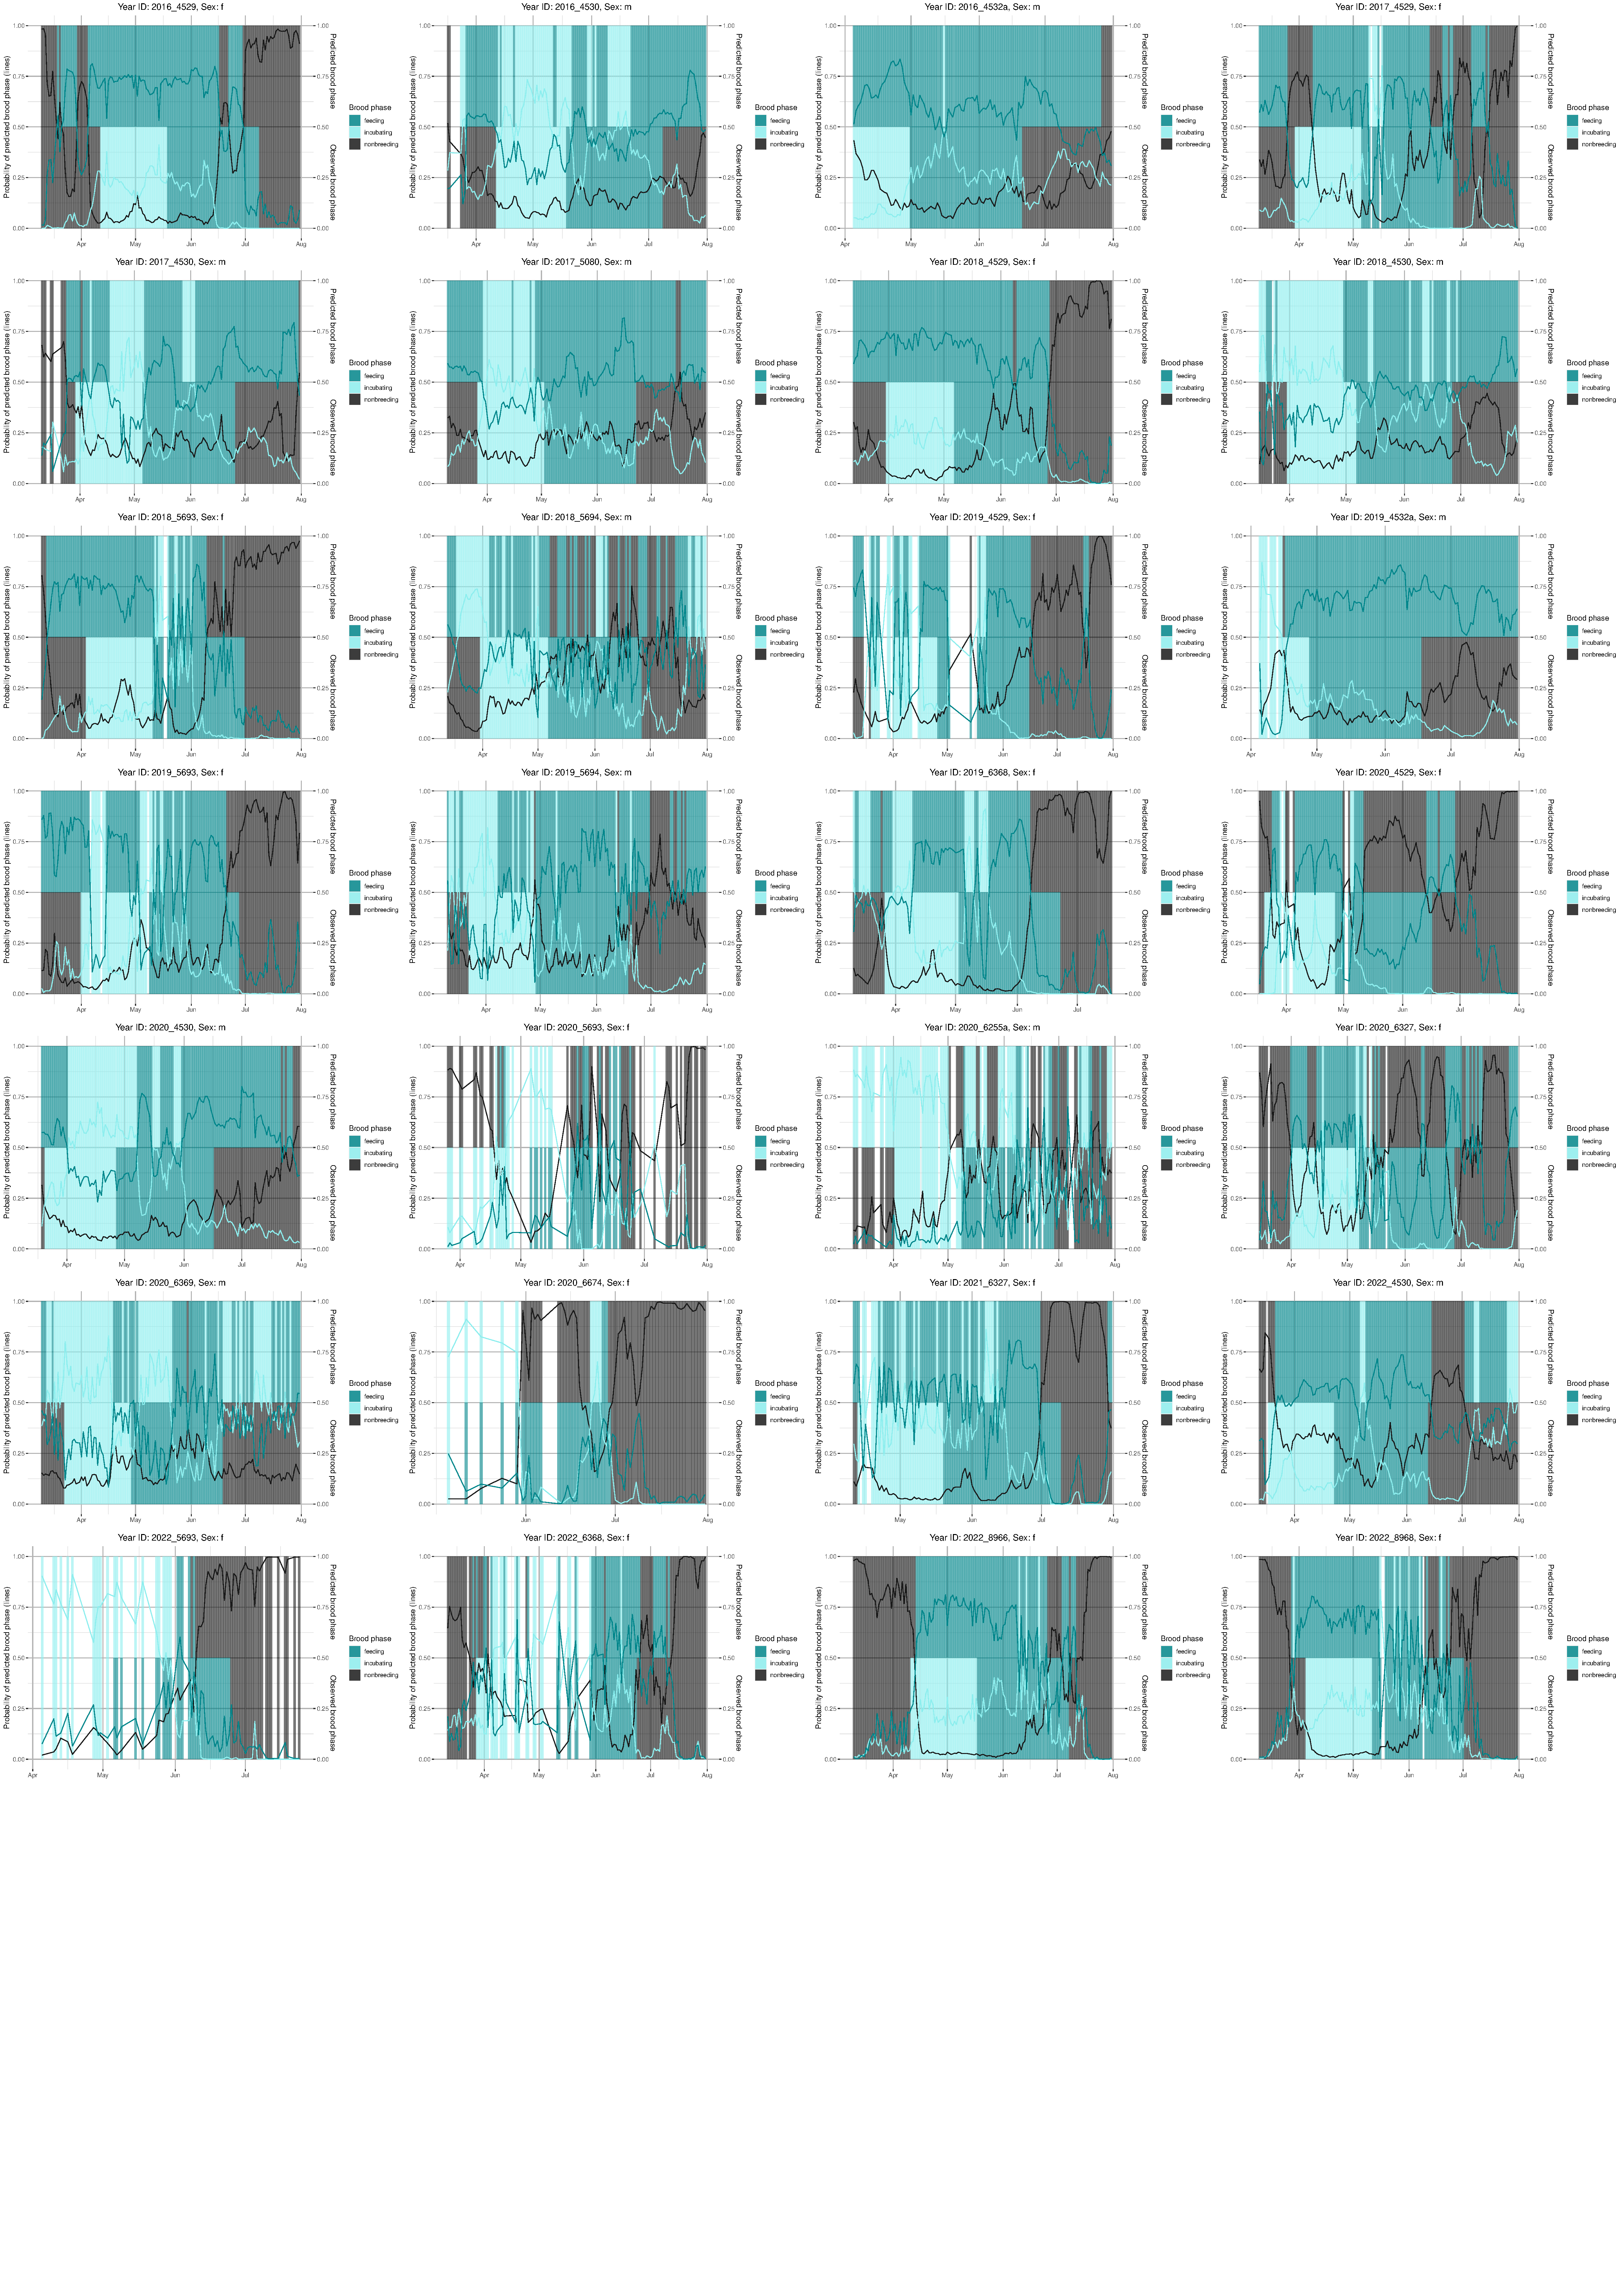
\includegraphics[width=1\textwidth]{figures/appendix/04_predictions_thuringia.pdf}
\end{figure}

\newpage
\phantomsection
\addcontentsline{toc}{section}{Personal Declaration}
\section*{Personal Declaration}
\vspace{2\baselineskip}

\noindent I hereby declare that the submitted thesis is the result of my own, independent work. All external sources are explicitly acknowledged in the thesis.
\vspace{4\baselineskip}

\noindent Place \& Date \hspace{54mm} Signature of the author

\vspace{2\baselineskip}

\noindent \begin{tabular}{@{}p{50mm}p{20mm}p{50mm}@{}}
Zurich, 30.04.2023\\
\hrulefill && \hrulefill
\end{tabular}

\end{document}